%!TEX program = xelatex
\documentclass[11pt,a4paper]{article}
\usepackage[utf8]{inputenc}
\usepackage[T1]{fontenc}
\usepackage{authblk}
\usepackage{tikz}
\usepackage{pgfplots}
\usepackage{verbatim}
\usepackage{amsfonts}
\usepackage{amsmath}
\usepackage{amsthm}
\usepackage{indentfirst}
\usepackage{amssymb}
\usepackage{enumerate}
\linespread{1.6}
\setlength{\footskip}{20pt}
\setlength{\parindent}{0pt}
\usetikzlibrary{shapes,snakes}
\newcommand{\argmax}{\operatornamewithlimits{argmax}}
\newcommand{\argmin}{\operatornamewithlimits{argmin}}

\DeclareMathOperator{\col}{col}
\usepackage{booktabs}
\newtheorem{theorem}{Theorem}
\newtheorem{proposition}{Proposition}
\newtheorem{lemma}{Lemma}
\newtheorem{example}{Example}
\newtheorem{corollary}{Corollary}
\newtheorem{definition}{Definition}
\newtheorem{note}{Note}
\newtheorem{claim}{Claim}
\usepackage{graphicx}
\usepackage{geometry}
\usepackage{hyperref}
\newcommand{\code}{	exttt}
\geometry{a4paper,scale=0.8}
\title{Optimization Methods}
\author[*]{Wenxiao Yang}
\affil[*]{Department of Mathematics, University of Illinois at Urbana-Champaign}
\date{Last updated: 2022.8.26}





\begin{document}
\maketitle
\tableofcontents
\newpage

\section{Unconstrained Optimization}
Function: $f:\mathbb{R}^n \rightarrow	\mathbb{R}^n$, $x\in \&,\ \&\subseteq \mathbb{R}^n$.

Terminology: $x^*$ will always be the optimal input at some function.

\subsection{Basic Definitions}
\subsubsection{Optimization in a Set}
$$\begin{array}{ll}\text { minimize } & f(x) \\ \text { subject to } & x \in X\end{array}$$
- Objective function $f: \mathbb{R}^{n} \rightarrow \mathbb{R}$ is a continuous function

- Optimization variable $x \in X$

- Local minimum of $f$ on $X: \exists \epsilon>0$ s.t. $f(x) \geq f(\hat{x})$, for all $x \in X$ such that $\|x-\hat{x}\| \leq \epsilon$;

i.e., $x^{*}$ is the best in the intersection of a small neighborhood and $X$

- Global minimum of $f$ on $X: f(x) \geq f\left(x^{*}\right)$ for all $x \in X$

"Strict global minimum", "strict local minimum" "local maximum", "global maximum" of $f$ on $X$ are defined accordingly

\subsubsection{Minimizer}
\begin{definition}
    \quad\\
    Say $x^*$ is a \underline{global minimizer(minimum)} of $f$ if $f(x^*)\leq f(x), \forall x\in \&$.

    Say $x^*$ is a \underline{unique global minimizer(minimum)} of $f$ if $f(x^*)< f(x), \forall x\neq x^*$.

    Say $x^*$ is a \underline{local minimizer(minimum)} of $f$ if $\exists r>0$ so that $f(x^*)\leq f(x)$ when $\|x-x^*\|<r$.
\end{definition}

A minimizer is \underline{strict} if $f(x^*)< f(x)$ for all relevant $x$.

\subsubsection{Stationary Point, Saddle Point}
All points $x^*$ s.t. $\nabla f(x^*)=0$ are called \underline{stationary points}.

Thus, all extrema are stationary points.

But not all stationary points have to be extrema.

\underline{Saddle points} are the stationary points neither local minimum nor local maximum.

\begin{example}
$f(x)=x^3$, $x=0$ is a stationary point but not extrema. (saddle point)
\end{example}

\subsubsection{Conditions for Global Optimality}
\textbf{Claim 1}: Consider a differentiable function $f$. Suppose:

(C1) $f$ has at least one global minimizer;

(C2) The set of stationary points is $S$, and $f\left(x^{*}\right) \leq f(x), \forall x \in S$.

Then $x^{*}$ is a global minimizer of $f^{*}$.
\begin{proof}
\quad\\
Suppose $\hat{x}$ is a global minimizer of $f$, i.e.,
$$
f(\hat{x}) \leq f(x), \forall x .
$$
By the necessary optimality condition, we have $\nabla f(\hat{x})=0$, thus $\hat{x} \in S$. By (C2), we have
$$
f\left(x^{*}\right) \leq f(\hat{x}) .
$$
Combining the two inequalities, we have $f(\hat{x}) \leq f\left(x^{*}\right) \leq f(\hat{x})$, thus $f(\hat{x})=f\left(x^{*}\right)$. Plugging into the second inequality, we have $f\left(x^{*}\right) \leq f(x), \forall x$. Thus $x^{*}$ is a global minimizer of $f^{*} .$
\end{proof}

\subsection{Special Situations: $\mathbb{R}, \mathbb{R}^n$}
\subsubsection{Optimization in $\mathbb{R}$}
\subsection*{Necessary condition of local-min: local minimizer $\Rightarrow f'(x^*)=0$}

\begin{theorem}
If $f(x)$ is differentiable function on interval $I$ and $x^*$ is a local minimizer, then either $x^*$ is an endpoint of $I$ or $f'(x^*)=0$.
\end{theorem}

\begin{proof}
Suppose $x^*$ is a local-min of $f$ and not an endpoint of $I$.

Def of $f'(x)=\lim_{h \rightarrow 0} \frac{f(x+h)-f(x)}{h}$\\
Def of local minimizer: $f(x^*)-f(x)\geq 0, |x^*-x|<r$\\
when $0<h<r$, $\frac{f(x+h)-f(x)}{h}\geq 0$; when $-r<h<0$, $\frac{f(x+h)-f(x)}{h}\leq 0$. Then $f'(x)=0$.
\end{proof}

\subsubsection*{Sufficient condition of local-min: $f'(x^*)=0, f''(x^*)\geq 0 \Rightarrow$ local minimizer}

\subsubsection*{Sufficient condition of global-min: $f'(x^*)=0, f''(x)\geq 0,\forall x\in I \Rightarrow$ local minimizer}
\begin{theorem}
    If $f:\mathbb{R} \rightarrow \mathbb{R}$ is a function with a continuous second derivative and $x^*$ is a critical point of $f$ (i.e. $f'(x)=0$), then:\\
    (1): If $f''(x)\geq 0,\ \forall x\in\mathbb{R}$, then $x^*$ is a global minimizer on $\mathbb{R}$.\\
    (2): If $f''(x)\geq 0,\ \forall x\in[a,b]$, then $x^*$ is a global minimizer on $[a,b]$.\\
    (3): If we only know $f''(x^*)\geq 0$, $x^*$ is a local minimizer.
\end{theorem}
\begin{proof}
\quad\\
(1)$f(x)=f(x^*)+f'(x^*)(x-x^*)+\frac{1}{2}f''(\xi)(x-x^*)^2=f(x^*)+0+\textit{something non negative}\geq f(x^*)\  \forall x$\\
(2) Similar to (1)\\
(3)$f''(x^*)\geq 0,\ f''$ continuous $\Rightarrow \exists r$ s.t. $f''(x)\geq 0$ $\forall x\in[x^*-\frac{r}{2},x^*+\frac{r}{2}]$, then $x$ is a local minimizer.
\end{proof}


\subsubsection{Optimization in $\mathbb{R}^n$}
\subsection*{First-order necessary condition of local-min: $\nabla f(x^*)=0$}
A base point $x$, we consider an arbitrary direction $u$. $\{x+tu| t\in \mathbb{R}\}$

For $\alpha>0$ sufficiently small:
\begin{enumerate}
    \item $f(x^*)\leq f(x^*+\alpha u)$
    \item $g(\alpha)=f(x^*+tu)-f(x^*)\geq 0$
    \item $g(\beta)$ is continuously differentiable for $\beta\in[0,\alpha]$
\end{enumerate}

By chain rule, $$g'(\beta)=\sum_{i=1}^n \frac{\partial f}{\partial x_i}(x^*+\beta u)u_i$$

By Mean Value Theorem, $$g(\alpha)=g(0)+g'(\beta)\alpha\text{ for some }\beta\in[0,\alpha]$$
Thus $$g(\alpha)=\alpha\sum_{i=1}^n \frac{\partial f}{\partial x_i}(x^*+\beta u)u_i\geq 0$$
$$\Rightarrow \sum_{i=1}^n \frac{\partial f}{\partial x_i}(x^*+\beta u)u_i\geq 0$$
Letting $\alpha \rightarrow	0$ and hence $\beta \rightarrow	0$, we get $$\sum_{i=1}^n \frac{\partial f}{\partial x_i}(x^*)u_i\geq 0\text{ for all }u\in \mathbb{R}^n$$
By choosing $u=[1,0,...,0]^T$, $u=[-1,0,...,0]^T$, we get $$\frac{\partial f(x^*)}{\partial x_1}\geq 0,\ \frac{\partial f(x^*)}{\partial x_1}\leq 0 \Rightarrow	\frac{\partial f(x^*)}{\partial x_1}= 0$$
Similarly, we can get $$\nabla f(x^*)=[\frac{\partial f(x^*)}{\partial x_1},\frac{\partial f(x^*)}{\partial x_2},...,\frac{\partial f(x^*)}{\partial x_n}]^T=0$$

\begin{theorem}
If $f$ is continuously differentiable and $x^*$ is a local extremum. Then $\nabla f(x^*)=0$.
\end{theorem}

\subsection*{Second-order necessary condition of local-min: $\nabla^2 f(x^*)\succeq 0$}
\begin{definition}
The Hessian of $f$ at point $x$ is an $n\times n$ symmetric matrix denoted by $\nabla^2 f(x)$ with $[\nabla^2 f(x)]_{ij}=\frac{\partial^2 f(x)}{\partial x_i\partial x_j}$
\end{definition}
\begin{theorem}
Suppose $f$ is twice continuously differentiable and $x^*$ in local \underline{minimum}. Then $$\nabla f(x^*)=0\text{ and }\nabla^2 f(x^*)\succeq 0$$
\end{theorem}
\begin{proof}
\quad\\
$\nabla f(x^*)=0$ already proved before.

Let $\alpha$ be small enough so that $g(\alpha)=f(x^*+\alpha u)-f(x^*)\geq 0$.

By Taylor series expansion,
\begin{equation}
    \begin{aligned}
        g(\alpha)&=g(0)+\alpha g'(0)+\frac{\alpha^2}{2}g''(0)+O(\alpha^2)\\
        g'(\alpha)&=\sum_{i=1}^n \frac{\partial f}{\partial x_i}(x^*+\beta u)u_i=\nabla f(x^*+\alpha u)^T u\\
        g''(\alpha)&=\sum_{i=1}^n\sum_{j=1}^n \frac{\partial^2 f}{\partial x_i\partial x_j}(x^*+\beta u)u_iu_j=u^T\nabla^2 f(x^*+\alpha u) u
    \end{aligned}
    \nonumber
\end{equation}
\begin{equation}
    \begin{aligned}
        g'(0)=\nabla f(x^*)^T u=0;\ g''(0)=u^T\nabla^2 f(x^*) u\\
        g(\alpha)=\frac{\alpha^2}{2}u^T\nabla^2 f(x^*) u+O(\alpha^2)\geq 0\\
        \text{When }\alpha \rightarrow 0,\text{ we get } u^T\nabla^2 f(x^*) u\geq 0,\ \forall u\in \mathbb{R}^n\\
        \Rightarrow	\nabla^2 f(x^*)\succeq 0
    \end{aligned}
    \nonumber
\end{equation}
\end{proof}

\subsection*{Sufficient condition of local-min: $\nabla f(x^*)=0\text{ and }\nabla^2 f(x^*)\succ 0$}
\begin{theorem}
Suppose $f$ is twice continuously differentiable in a neighborhood of $x^*$ and
(1) $\nabla f(x^*)=0$; (2) $\nabla^2 f(x^*)\succ 0$ ($u^T\nabla^2 f(x^*) u>0$, $\forall u\in \mathbb{R}^n$).
Then $x^*$ is local minimum.
\end{theorem}
\begin{proof}
\quad\\
Consider $u\in \mathbb{R}^n$, $\alpha>0$ and let
\begin{equation}
    \begin{aligned}
        g(\alpha)&=f(x^*+\alpha u)-f(x^*)\\
        &=\frac{\alpha^2}{2}u^T\nabla^2 f(x^*) u+O(\alpha^2)\geq 0\\
        &=\frac{\alpha^2}{2}[u^T\nabla^2 f(x^*) u+2\frac{O(\alpha^2)}{\alpha^2}]\\
        &u^T\nabla^2 f(x^*) u>0;\ \frac{O(\alpha^2)}{\alpha^2}\rightarrow 0\\
        &\Rightarrow g(\alpha)>0\text{ for }\alpha\text{ sufficiently small for all }u\neq 0\\
        &\Rightarrow x^*\text{ is local minimum}.
    \end{aligned}
    \nonumber
\end{equation}

(specially if $\|u\|=1$, $u^T\nabla^2 f(x^*) u\geq \lambda_{\min}(\nabla^2 f(x^*))$, $\lambda_{\min}(\nabla^2 f(x^*))$ is the minimal eigenvalues of $\nabla^2 f(x^*)$.)
\end{proof}






\subsubsection{Using Optimality Conditions to Find Minimum in $\mathbb{R}^n$}
\begin{enumerate}
    \item Find all points satisfying necessary condition $\nabla f(x)=0$ (all stationary points)
    \item Filter out points that don't satisfy $\nabla^2 f(x)\geq 0$
    \item Points with $\nabla^2 f(x)> 0$ are strict local minimum.
    \item Among all points with $\nabla^2 f(x)\geq 0$, declare a global minimum, one with the smallest value of $f$, assuming that global minimum exists.
\end{enumerate}
\begin{example}
$f(x)=2x^2-x^4$
\end{example}
\begin{equation}
    \begin{aligned}
        f'(x)&=4x-4x^3=0\\
        \Rightarrow& x=0,x=1,x=-1\text{ are stationary points}\\
        f''(x)&=4-12x^2=\left\{\begin{matrix}
            4&\text{if }x=0\\
            -8&\text{if }x=1,-1
        \end{matrix}\right.\\
        \Rightarrow	&x=0\text{ is the only local min, and it is strict}
    \end{aligned}
    \nonumber
\end{equation}
But $-f(x) \rightarrow \infty$ as $|x|\rightarrow \infty \Rightarrow$ no global min, but global max exists. $f(1),f(-1)$ are strict local max and both global max.

\subsection{Existence of Global-min}
\subsubsection{(Bolzano-)Weierstrass Theorem: Compact set $X$ $\Rightarrow$ $\exists$ global-min/max}
\begin{theorem}[Bolzano-Weierstrass Theorem (compact domain)]
    Any continuous function $f$ has at least one global minimizer on any \textbf{compact set} $X$.

    That is, there exists an $x^{*} \in X$ such that $f(x) \geq f\left(x^{*}\right), \forall x \in X$.
\end{theorem}

\begin{corollary}[bounded level sets]
    Suppose $f: \mathbb{R}^{d} \rightarrow \mathbb{R}$ is a continuous function. If for a certain $c$, the level set
    $$
    \{x \mid f(x) \leq c\}
    $$
    is \textbf{non-empty} and \textbf{compact}, then the global minimizer of $f$ exists, i.e., there exists $x^{*} \in \mathbb{R}^{d}$ s.t.
    $$
    f\left(x^{*}\right)=\inf _{x \in \mathbb{R}^{d}} f(x)
    $$
\end{corollary}
\begin{example}
    $f(x) = x^2$.
    Level set $\{x|x^2 \leq 1\}$ is $\{x|-1\leq x\leq 1\}$: non-empty compact. Thus, there exists a global minimum.
\end{example}

\subsubsection{Coercive function $f$ $\Rightarrow$ $\exists$ global-min}
\begin{corollary}[coercive]
    Suppose $f: \mathbb{R}^{d} \rightarrow \mathbb{R}$ is a continuous function. If $f$ is coercive ($f(x) \rightarrow \infty$ as $\|x\| \rightarrow \infty$), then the global minimizer of $f$ over $\mathbb{R}^{d}$ exists.
\end{corollary}
\begin{proof}
Let $\alpha\in \mathbb{R}^d$ be chosen so that the set $S = \{x |f(x) \leq \alpha\}$ is non-empty. By coercivity,
this set is compact.
\end{proof}
Coercive $\Rightarrow$ one non-empty bounded level set; but not the other way.

Claim (all level sets bounded $\Leftrightarrow$ coercive): Let $f$ be a continuous function, then $f$ is coercive iff $\{x | f(x) \leq \alpha\}$ is compact for any $\alpha$.

\subsection{Method of finding-global-min-among-stationary-points (FGMSP)}
Method of finding-global-min-among-stationary-points (FGMSP):

Step 0: Verify coercive or bounded level set:

- Case 1: success, go to Step $1 .$

- Case 2: otherwise, try to show non-existence of global-min. If success, exit and report "no global-min exists".

- Case 3: cannot verify coercive or bounded level set; cannot show non-existence of global-min. Exit and report "cannot decide".

Step 1: Find all stationary points (candidates) by solving $\nabla f(\mathbf{x})=0$;

Step 2 (optional): Find all candidates s.t. $\nabla^{2} f(\mathbf{x}) \succeq 0$.

Step 3: Among all candidates, find one candidate with the minimal value. Output this candidate, and report "find a global $\mathrm{min}$ ".






\section{Function}
\subsection{Convexity}
\subsubsection{Definition}
\begin{center}
    \fcolorbox{black}{gray!10}{\parbox{.9\linewidth}{\underline{\textbf{Convex set}} $C: x, y \in C$ implies $\lambda x+(1-\lambda) y \in C$, for any $\lambda \in[0,1]$.

    \underline{\textbf{Convex function} (0-th order)}: $f$ is convex in a convex set $C$ iff $f(\alpha x+(1-\alpha) y) \leq \alpha f(x)+(1-\alpha) f(y), \forall x, y \in C, \forall \alpha \in[0,1] .$
    
    A function $f$ is a \underline{\textbf{concave function}} iff $-f$ is a convex function.}
    }
\end{center}

Alternative definitions of \underline{convex function} $f$:
\begin{enumerate}[(1)]
    \item (differentiable): $f(z) \geq f(x)+(z-x)^{T} \nabla f(x), \ \forall x, z \in C .$
    \item (twice differentiable): $\nabla^{2} f(x) \succeq 0,\ \forall x \in C .$
\end{enumerate}

\textbf{Property (1st order)}: If $f$ is differentiable, then $f$ is convex iff $f(z) \geq f(x)+(z-x)^{T} \nabla f(x), \ \forall x, z \in C .$ The inequality is strict for strict convexity.
\begin{proof}
\quad
\begin{enumerate}[(i)]
    \item "$\Rightarrow$" \begin{equation}
        \begin{aligned}
            f(x+\alpha (y-x))&\leq (1-\alpha)f(x)+\alpha f(y), \forall \alpha \in (0,1)\\
            \Rightarrow	\frac{f(x+\alpha(y-x))-f(x)}{\alpha}&\leq f(y)-f(x)\\
            \text{Limit as }\alpha \rightarrow 0 \Rightarrow (y-x)^{T} \nabla f(x)&\leq f(y)-f(x)
        \end{aligned}
        \nonumber
    \end{equation}
    \item "$\Leftarrow$" Let $g=\alpha x+(1-\alpha) y$
    \begin{equation}
        \begin{aligned}
            f(g)+(x-g)^{T} \nabla f(g)&\leq f(x)\\
            f(g)+(y-g)^{T} \nabla f(g)&\leq f(y)\\
            \Rightarrow	f(g)&\leq \alpha f(x)+(1-\alpha)f(y)\\
            f(\alpha x+(1-\alpha) y)&\leq \alpha f(x)+(1-\alpha)f(y)
        \end{aligned}
        \nonumber
    \end{equation}
\end{enumerate}
\end{proof}

\textbf{Property (2nd order)}: If $f$ is twice differentiable, then $f$ is convex iff
$$
\nabla^{2} f(x) \succeq 0,\ \forall x \in C .
$$
Strictly convex: $\nabla^{2} f(x) \succ 0,\ \forall x \in C \Rightarrow	$ $f$ is strictly convex.

\textbf{Note:} $f$ is strictly convex $\nRightarrow \nabla^{2} f(x) \succ 0$.
\begin{example}
$f(x)=x^4\text{(strictly convex)}$, $\frac{d^2f(x)}{dx^2}=12x^2(=0\text{ at }x=0)$
\end{example}

\textbf{Convex set graph}:
\begin{center}\begin{figure}[htbp]
    \centering
    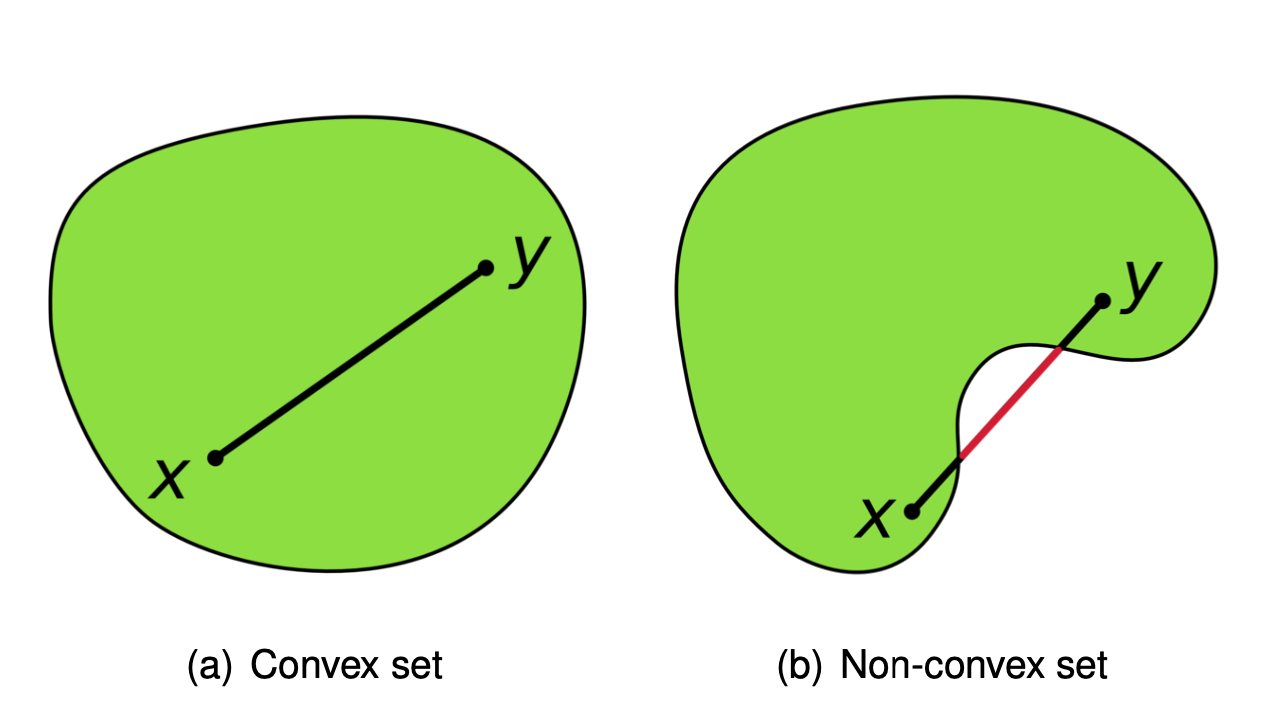
\includegraphics[scale=0.3]{Convex_set.png}
    \caption{}
    \label{}
\end{figure}\end{center}

\subsubsection{Properties}
Convex functions $f$ over $\mathbb{R}^n$, $\{f_i\}_{i\in \mathbb{Z}}$ over $\&$:
\begin{enumerate}[(1)]
    \item $C=\{x\in \mathbb{R}^n| f(x)\leq a\}$ is convex set, $\forall a\in \mathbb{R}$.
    \item $f_{sum}(x)=\sum_{i=1}^kf_i(x)$ is convex over $\&$
    \item $f_{max}(x)=\max_{i=1,...,k}f_i(x)$ is convex over $\&$
\end{enumerate}
\begin{proof} Only prove (3) here:
\begin{equation}
    \begin{aligned}
        f_{max}(\alpha x+(1-\alpha)y)&=\max_{i=1,...,k}f_i(\alpha x+(1-\alpha)y)\\
    &\leq \max_{i=1,...,k}[\alpha f_i(x)+(1-\alpha)f_i(y)]\\
    &\leq \max_{i=1,...,k}\alpha f_i(x)+\max_{i=1,...,k}(1-\alpha)f_i(y)\\
    &=\alpha f_{max}(x)+(1-\alpha)f_{max}(y)
    \end{aligned}
    \nonumber
\end{equation}
\end{proof}












\subsubsection{Proposition: Convex function $f$, $\nabla f(x^*)=0$ $\Rightarrow$ global-min}
\begin{proposition}
    Let $f: X \longmapsto \mathbb{R}$ be a convex function over the convex set $X$.

    (a) A local-min of $f$ over $X$ is also a global-min over $X$. If $f$ is strictly convex,then min is unique.

    (b) If $X$ is open (e.g. $\mathbb{R}^{n}$ ), then $\nabla f\left(x^{*}\right)=0$ is a necessary and sufficient condition for $x^{*}$ to be a global minimum.
\end{proposition}
\begin{proof}
\quad\\
Proof based on a property: If $f$ is differentiable over $C$ (open), then $f$ is convex iff
$$
f(z) \geq f(x)+(z-x)^{\prime} \nabla f(x), \quad \forall x, z \in C .
$$
\end{proof}














\begin{corollary}
    Let $f: X \longmapsto \mathbb{R}$ be a concave function over the convex set $X$.

    (a) A local-max of $f$ over $X$ is also a global-max over $X$.

    (b) If $X$ is open (e.g. $\mathbb{R}^{n}$ ), then $\nabla f\left(x^{*}\right)=0$ is a necessary and sufficient condition for $x^{*}$ to be a global maximum.
\end{corollary}

\subsubsection{Application: Unconstrained Quadratic Optimization}
$$\begin{array}{ll}\text { minimize } & f(\mathbf{w})=\frac{1}{2} \mathbf{w}^{T} \mathbf{Q} \mathbf{w}-\mathbf{b}^{T} \mathbf{w} \\ \text { subject to } & \mathbf{w} \in \mathbb{R}^{d}\end{array}$$
where $\mathbf{Q}$ is a symmetric $d \times d$ matrix. (what if non-symmetric?)
$$\nabla f(\mathbf{w})=\mathbf{Q}\mathbf{w}-\mathbf{b},\ \nabla^2 f(\mathbf{w})=\mathbf{Q}$$
\begin{enumerate}[(i)]
    \item $\mathbf{Q}\succeq 0 \Leftrightarrow	f$ is convex.
    \item $\mathbf{Q}\succ 0 \Leftrightarrow	f$ is strictly convex.
    \item $\mathbf{Q}\preceq 0 \Leftrightarrow	f$ is concave.
    \item $\mathbf{Q}\prec 0 \Leftrightarrow	f$ is strictly concave.
\end{enumerate}









- Necessary condition for (local) optimality
$$
\mathbf{Q} \mathbf{w}=\mathbf{b}, \quad \mathbf{Q} \succeq 0
$$

Case 1: $\mathbf{Q w}=\mathbf{b}$ has no solution, i.e. $\mathbf{b} \notin R(\mathbf{Q})$. No stationary point, no lower bound ($f$ can achieve $-\infty$).

Case 2: $\mathbf{Q}$ is not PSD ( $f$ is non-convex)
No local-min, no lower bound ($f$ can achieve $-\infty$).

Case 3: $\mathbf{Q} \succeq 0$ (PSD) and $\mathbf{b} \in R(\mathbf{Q})$. Convex, has global-min, 
any stationary point is a global optimal solution.

\begin{example}
    Toy Problem 1: $\min _{x, y \in \mathbb{R}} f(x, y) \triangleq x^{2}+y^{2}+\alpha x y$.
\end{example}
\begin{enumerate}
    \item Step 1: First order condition: $2 x^{*}+\alpha y^{*}=0,2 y^{*}+\alpha x^{*}=0$.
    
    - We get $4 x^{*}=-2 \alpha y^{*}=\alpha^{2} x^{*}$. So $\left(4-\alpha^{2}\right) x^{*}=0$.
    
    - Case 1: $\alpha^{2}=4$. If $x^{*}=-\alpha y^{*} / 2$, then $\left(x^{*}, y^{*}\right)$ is a stationary point.
    
    - Case 2: $\alpha^{2} \neq 4$. Then $x^{*}=0 ; y^{*}=-\alpha x^{*} / 2=0$. So $(0,0)$ is stat-pt.
    \item Step 2: Check convexity. Hessian $\nabla^{2} f(x, y)=\left(\begin{array}{ll}2 & \alpha \\ \alpha & 2\end{array}\right)$.
    
    Eigenvalues $\lambda_{1}, \lambda_{2}$ satisfy $\left(\lambda_{i}-2\right)^{2}=\alpha^{2}, i=1,2$.
    Thus $\lambda_{1,2}=2 \pm|\alpha|$.

    - If $|\alpha| \leq 2$, then $\lambda_{i} \geq 0, \forall i$. Thus $f$ is convex. Any stat-pt is global-min.

    - If $|\alpha|>2$, at least one $\lambda_{i}<0$, thus $f$ is not convex.
    \item Step 3 (can be skipped now): For non-convex case $(|\alpha|>2)$, prove no lower bound.
    
    $f(x, y)=(x+\alpha y / 2)+\left(1-\alpha^{2} / 4\right) y^{2}$. Pick $y=M, x=-\alpha M / 2$, then
    $f(x, y)=\left(1-\alpha^{2} / 4\right) M^{2} \rightarrow-\infty$ as $M \rightarrow \infty$.
\end{enumerate}

Summary:

If $|\alpha|>2$, no global-min, $(0,0)$ is stat-pt;

if $|\alpha|=2$, any $(-0.5 \alpha t, t), t \in \mathbb{R}$ is a stat-pt and global-min;

if $|\alpha|<2,(0,0)$ is the unique stat-pt and global-min.

\begin{example}
Linear Regression
\end{example}
$\text{minimize } f(\mathbf{w})=\frac{1}{2}\left\|\mathbf{X}^{T} \mathbf{w}-\mathbf{y}\right\|^{2}$ subject to $ \mathbf{w} \in \mathbb{R}^{d}$

$n$ data points, $d$ features

- $\mathbf{X}$ may be wide (under-determined), tall (over-determined), or rank-deficient

- Note that comparing with the previous case, $\mathbf{Q}=\mathbf{X X}^{T} \in \mathbb{R}^{d \times d}$, $\mathbf{b}=\mathbf{X} \mathbf{y} \in \mathbb{R}^{d \times 1}$

- $\mathbf{Q} \succeq 0$; Case 2 never happens!

- First order condition $\mathbf{X X}^{\top} \mathbf{w}^{*}=\mathbf{X} \mathbf{y}$.

\quad - It always has a solution; Case 1 never happens!

\textbf{Claim}: Linear regression problem is always convex; it has global-min.

First order condition
$$
\mathbf{X X}^{\top} \mathbf{w}^{*}=\mathbf{X} \mathbf{y}
$$
which always has a solution.

If $X X^{\top} \in \mathbb{R}^{d \times d}$ is invertible (only happen when $n \geq d$ ), then there is a unique stationary point $x=\left(A^{\top} A\right)^{-1} A^{\top} b$. It is also a global minimum.

If $X X^{\top} \in \mathbb{R}^{d \times d}$ is not invertible, then there can be infinitely many stationary points, which are the solutions to the linear equation.
All of them are global minima, giving the same function value.

\subsection{Strongly Convexity}
\subsubsection{$\mu$-Strongly Convex: $
\langle\nabla f(w)-\nabla f(v), w-v\rangle \geq \mu\|w-v\|^{2}$}
\textbf{Definition}: We say $f: C \rightarrow \mathbb{R}$ is a $\mu$-strongly convex function in a convex set $C$ if $f$ is differentiable and
$$
\langle\nabla f(w)-\nabla f(v), w-v\rangle \geq \mu\|w-v\|^{2}, \quad \forall w, v \in C .
$$
\subsubsection{$\mu$-strongly convex $\Leftrightarrow \nabla^{2} f(x) \succeq \mu I\Leftrightarrow$"$f(x)-m\|x\|^2$ is convex"}
If $f$ is twice differentiable, then $f$ is $\mu$-strongly convex iff
$$
\nabla^{2} f(x) \succeq \mu I, \quad \forall x \in C .
$$
\begin{definition}
    A twice continuously differentiable function is \underline{strongly convex} if $$\exists m>0\text{ s.t. }\nabla^2 f(x)\succeq mI\quad \forall x$$
    which is also called $m-$strongly convex.

    \textbf{(alternative):} "$f(x)-m\|x\|^2$ is convex" is also an equivalent definition for $f(x)$ is $m-$strongly convex.
\end{definition}

Namely, all eigenvalues of the Hessian at any point is at least $\mu$.

if $f(w)$ is convex, then $f(w)+\frac{\mu}{2}\|w\|^{2}$ is $\mu$-strongly convex.

- In machine learning, easy to change a convex function to a strongly convex function: just add a regularizer

\subsubsection{Lemma: Strongly convexity $\Rightarrow$ Strictly convexity}
\begin{lemma}
    Strongly convexity $\Rightarrow$ Strictly convexity.
\end{lemma}
\begin{proof}
\begin{equation}
    \begin{aligned}
        \nabla^2 f(x)&\succeq mI \Rightarrow \nabla^2 f(x)-mI\succeq 0\\
        & \Rightarrow \forall z\neq 0\quad z^T(\nabla^2 f(x)-mI)z\geq 0\\
        & \Rightarrow z^T\nabla^2 f(x)z\geq mz^Tz>0
    \end{aligned}
    \nonumber
\end{equation}
\end{proof}
\textbf{Note: }converse is not true: e.g. $f(x)=x^4$ is strictly convex but $\nabla^2 f(0)=0$

\subsubsection{Lemma: $\nabla^2 f(x)\succeq mI$ $\Rightarrow$ $f(y)\geq f(x)+\nabla f(x)^T(y-x)+\frac{m}{2}\|y-x\|^2$}
\begin{lemma}
$\nabla^2 f(x)\succeq mI\quad \forall x$

$$\Rightarrow f(y)\geq f(x)+\nabla f(x)^T(y-x)+\frac{m}{2}\|y-x\|^2$$
\end{lemma}
\begin{proof}
    By Taylor's Theorem,
    \begin{equation}
        \begin{aligned}
            f(y)&=f(x)+\nabla f(x)^T(y-x)+\frac{1}{2}(y-x)^T \nabla^2 f((1-\beta)x+\beta y)(y-x),\quad \text{for some }\beta\in[0,1]\\
            &\geq f(x)+\nabla f(x)^T(y-x)+\frac{1}{2}(y-x)^Tm(y-x)\\
            &\geq f(x)+\nabla f(x)^T(y-x)+\frac{m}{2}\|y-x\|^2
        \end{aligned}
        \nonumber
    \end{equation}
\end{proof}



\subsection{Lipschitz Gradient ($L$-Smooth)}
\begin{definition}[Lipschitz Continunity]
A function $g: \mathbb{R}^n \rightarrow	\mathbb{R}^m$ is called Lipschitz (continuous) if $\exists L>0$ s.t.
$$\|g(y)-g(x)\|\leq L\|y-x\|,\forall x,y\in \mathbb{R}^n$$
$L$ is Lipschitz constant.
\end{definition}

\begin{definition}[Lipschitz Gradient]
    $\nabla f(x)$ is Lipschitz if $\exists L>0$ s.t. $$\|\nabla f(x)-\nabla f(y)\|\leq L\|x-y\|,\forall x,y\in \mathbb{R}^n$$
\end{definition}
We can say $f$ is $L$-Smooth.

\begin{example}
    \quad

\begin{enumerate}
    \item $f(x)=\|x\|^4$, $\nabla f(x)=4\|x\|^2x$
    
    Test $\|\nabla f(x)-\nabla f(-x)\|\leq L\|2x\|$, $8\|x\|^2\|x\|\leq 2L\|x\|$ which doesn't hold when $\|x\|^2>\frac{L}{4}$.
    \item If $f$ is twice continuously differentiable with $\nabla^2 f(x)\succeq -MI$ and $\nabla^2 f(x)\preceq  MI$ then $\|\nabla f(x)-\nabla f(y)\|\leq M\|x-y\|,\forall x,y\in \mathbb{R}^n$. ($A\succeq B$ means $A-B\succeq 0$, $A\preceq B$ means $A-B\preceq 0$)
\end{enumerate}
\end{example}

\subsubsection{Theorem: $-MI\preceq\nabla^2 f(x)\preceq  MI$ $\Rightarrow$ $f$ is $M$-smooth}
\begin{theorem}
$-MI\preceq\nabla^2 f(x)\preceq  MI, \forall x \Rightarrow \|\nabla f(x)-\nabla f(y)\|\leq M\|x-y\|,\forall x,y$
\end{theorem}
\begin{proof}
For symmetric $A$,
\begin{enumerate}
    \item $x^TAx\leq \lambda_{\max}(A)\|x\|^2$
    \item $\lambda_{i}(A^2)=\lambda_i^2(A)$
    \item $-MI\preceq A\preceq  MI \Rightarrow \lambda_{\min}(A)\geq-M,\lambda_{\max}(A)\leq M$
\end{enumerate}
Define $g(t)=\frac{\partial f}{\partial x_i}(x+t(y-x))$. Then
\begin{equation}
    \begin{aligned}
        g(1)&=g(0)+\int_0^1g'(s)ds\\
        \Rightarrow	\frac{\partial f(y)}{\partial x_i}&=\frac{\partial f(x)}{\partial x_i}+\int_0^1\sum_{j=1}^n \frac{\partial^2 f(x+s(y-x))}{\partial x_i\partial x_j}(y_j-x_j)ds\\
        \nabla f(y)&=\nabla f(x)+\int_0^1 \nabla^2 f(x+s(y-x))(y-x)ds\\
        \|\nabla f(y)-\nabla f(x)\|&=\|\int_0^1 \nabla^2 f(x+s(y-x))(y-x)ds\|\\
        &\leq \int_0^1\|\nabla^2 f(x+s(y-x))(y-x)\|ds\\
        &=\int_0^1\sqrt{(y-x)^T[\nabla^2 f(x+s(y-x))]^2(y-x)}ds\\
        &(\text{Set }H=\nabla^2 f(x+s(y-x)))\\
        &\leq \int_0^1\sqrt{\lambda_{\max}(H^2)\|y-x\|^2}ds\\
        &\leq M\|y-x\|
    \end{aligned}
    \nonumber
\end{equation}
\end{proof}

\subsubsection{Descent Lemma: $f$ is $L$-smooth $\Rightarrow$ $f(y)\leq f(x)+\nabla f(x)^T(y-x)+\frac{L}{2}\|y-x\|^2$}
\begin{lemma}[Descent Lemma]
Let $f: \mathbb{R}^n \rightarrow \mathbb{R}$ be continuously differentiable with a Lipschitz gradient with Lipschitz constant $L$. Then
\begin{equation}
    \begin{aligned}
        f(y)\leq f(x)+\nabla f(x)^T(y-x)+\frac{1}{2}L\|y-x\|^2
    \end{aligned}
    \nonumber
\end{equation}
\end{lemma}
\begin{proof}
Let $g(t)=f(x+t(y-x))$. Then $g(0)=f(x)$ and $g(1)=f(y)$, $g(1)=g(0)+\int_0^1g'(t)dt$.

Where $g'(t)=\nabla f(x+t(y-x))^T(y-x)$

\begin{equation}
    \begin{aligned}
        \Rightarrow	f(y)&=f(x)+\int_0^1\nabla f(x+t(y-x))^T(y-x)dt\\
        &=f(x)+\int_0^1(\nabla f(x+t(y-x))-\nabla f(x))^T(y-x)dt+\nabla f(x)^T(y-x)\\
        &\leq f(x)+\int_0^1\|\nabla f(x+t(y-x))-\nabla f(x)\|\|y-x\|dt+\nabla f(x)^T(y-x)\\
        &\leq f(x)+L\int_0^1\|t(y-x)\|\|y-x\|dt+\nabla f(x)^T(y-x)\\
        &=f(x)+\frac{1}{2}L\|y-x\|^2+\nabla f(x)^T(y-x)
    \end{aligned}
    \nonumber
\end{equation}
\end{proof}

\subsubsection{Co-coercivity Condition: $(\nabla f(x)-\nabla f(y))^T(x-y)\geq \frac{1}{L}\|\nabla f(x)-\nabla f(y)\|^2$}
\begin{theorem}[Co-coercivity Condition]
Let $f$ be convex and continuously differentiable. Let $f$ be $L$-smooth. Then
\begin{equation}
    \begin{aligned}
        (\nabla f(x)-\nabla f(y))^T(x-y)\geq \frac{1}{L}\|\nabla f(x)-\nabla f(y)\|^2
    \end{aligned}
    \nonumber
\end{equation}
\end{theorem}
\begin{proof}
Let $y\in \mathbb{R}^n$, and define $g(x)=f(x)-\nabla f(y)^Tx$. Then $\nabla g(y)=\nabla f(y)-\nabla f(y)=0$ and $\nabla^2 g(y)=\nabla^2 f(y)\succeq 0$, i.e. $y$ minimize $g$. Because $g(y)\leq g(\cdot)$, $g(y)\leq g(x-\frac{1}{L}\nabla g(x))$
According to the descent lemma,
\begin{equation}
    \begin{aligned}
        g(x-\frac{1}{L}\nabla g(x))&=f(x-\frac{1}{L}\nabla g(x))-\nabla f(y)^T(x-\frac{1}{L}\nabla g(x))\\
        &\leq f(x)+\frac{L}{2}\|-\frac{1}{L}\nabla g(x)\|^2+\nabla f(x)^T(-\frac{1}{L}\nabla g(x))-\nabla f(y)^T(x-\frac{1}{L}\nabla g(x))\\
        &\leq f(x)+\frac{1}{2L}\|\nabla g(x)\|^2-(\nabla f(x)-\nabla f(y))^T\frac{1}{L}\nabla g(x)-\nabla f(y)^Tx\\
        &=f(x)-\frac{1}{2L}\|\nabla f(x)-\nabla f(y)\|^2-\nabla f(y)^Tx\\
        &=g(x)-\frac{1}{2L}\|\nabla f(x)-\nabla f(y)\|^2
    \end{aligned}
    \nonumber
\end{equation}
Then,
\begin{equation}
    \begin{aligned}
        g(y)\leq g(x-\frac{1}{L}\nabla g(x))=g(x)-\frac{1}{2L}\|\nabla f(x)-\nabla f(y)\|^2\\
        \Rightarrow	g(y)-g(x)=f(y)-\nabla f(y)^Ty-f(x)-\nabla f(y)^Tx\leq -\frac{1}{2L}\|\nabla f(x)-\nabla f(y)\|^2
    \end{aligned}
    \nonumber
\end{equation}
We can interchange $x,y$,
\begin{equation}
    \begin{aligned}
        \left\{\begin{matrix}
            f(y)-\nabla f(y)^Ty-f(x)-\nabla f(y)^Tx\leq -\frac{1}{2L}\|\nabla f(x)-\nabla f(y)\|^2\\
            f(x)-\nabla f(x)^Tx-f(y)-\nabla f(x)^Ty\leq -\frac{1}{2L}\|\nabla f(x)-\nabla f(y)\|^2
        \end{matrix}\right.
    \end{aligned}
    \nonumber
\end{equation}
Add these two inequalities together,
\begin{equation}
    \begin{aligned}
        (\nabla f(x)-\nabla f(y))^T(x-y)\geq \frac{1}{L}\|\nabla f(x)-\nabla f(y)\|^2
    \end{aligned}
    \nonumber
\end{equation}
\end{proof}











\section{Gradient Methods}
\begin{definition}[Iterative Descent]
Start at some point $x_0$, and successively generate $x_1,x_2,..$ s.t. $$f(x_{k+1})<f(x_k)\quad k=0,1,...$$
\end{definition}

\begin{definition}[\textbf{General Gradient Descent Algorithm}]
    Assume that $\nabla f(x_k)\neq 0$. Then
    $$x_{k+1}=x_k+\alpha_k d_k$$
    where $d_k$ is s.t. $d_k$ has a positive projection along $-\nabla f(x_k)$,
    $$\nabla f(x_k)^T d_k<0 \equiv -\nabla f(x_k)^T d_k>0$$
\end{definition}
\begin{enumerate}[$\bullet$]
    \item If $d_k=-\nabla f(x_k)$ we get \textbf{steepest descent}.
    \item Often $d_k$ is constructed using matrix $D_k \succ 0$ $$d_k=-D_k\nabla f(x_k)$$
\end{enumerate}

\subsection{Steepest Descent}
We want the $x_k$ that decreases the function most.
\begin{proposition}
$-\nabla f(x_k)$ is the direction deceases the function most.
\end{proposition}
\begin{proof}
Suppose the direction is $v\in \mathbb{R}^n, v\neq 0$.
$$f(x+\alpha v)=f(x)+\alpha v^T \nabla f(x)+O(\alpha)$$
The rate of change of $f$ along direction $v$:
$$\lim_{\alpha \rightarrow 0}\frac{f(x+\alpha v)-f(x)}{\alpha}=v^T\nabla f(x)$$
By Cauchy-schwarz inequality,
$$|v^T\nabla f(x)|\leq \|v\|\|\nabla f(x)\|$$
Equation holds when $v=\beta \nabla f(x)$. Hence, $-\nabla f(x)$ is the direction decreases the function most.
\end{proof}

\begin{definition}[\textbf{Steepest Descent Algorithm}]
$$x_{k+1}=x_k-\alpha_k \nabla f(x_k)$$
$\alpha_k$ is the step size, which need to choose carefully.
\end{definition}

\subsection{Methods for Choosing Step Size $\alpha_k$}
\begin{enumerate}[Method (1):]
    \item Fixed step size: $\alpha_k=\alpha$ (can have issue with \textit{convergence})
    \item \textbf{Optimal Line Search}: choose $\alpha_k$ to optimize the value of next iteration, i.e. solve $$\min_{\alpha\geq 0}f(x_k+\alpha d_k)$$ (may be \textit{difficult in practice})
    \item \textbf{Armijo's Rule} (successive step size reduction):$$f(x_k+\alpha_k d_k)=f(x_k)+\alpha_k \nabla f(x_k)^T d_k+O(\alpha_k)$$
    Since $\nabla f(x_k)^T d_k<0$, $f$ decreases when $\alpha_k$ is sufficiently small. But we also don't want $\alpha_k$ to be too small (slow).
\end{enumerate}

\subsection*{Optimal(Exact) Line Search}
\begin{example}
    (False $\times$) The gradient descent algorithm with an exact line search always finds the minimum of a strictly convex quadratic function in exactly one iteration.
\end{example}
Note: the moving direction is restricted to the gradient.

Counterexample: False. It is not necessary that the gradient at $x_{0}$ towards the exact solution. For example, let $f(x)=$ $\frac{1}{2} x^{\top} Q x+x^{\top} b$ where $Q=\left(\begin{array}{ll}2 & 0 \\ 0 & 1\end{array}\right)$ and $b=\left(\begin{array}{c}1 \\ -1\end{array}\right)$. Clearly we have $x^{*}=\left(\begin{array}{c}-1 / 2 \\ 1\end{array}\right)$. If we start with $x_{0}=\left(\begin{array}{l}1 \\ 2\end{array}\right)$, by using exact line search, the step size $\alpha=\arg \min f\left(x_{0}-\alpha \nabla f\left(x_{0}\right)\right)=10 / 19$. Hence $x_{1}=x_{0}-\alpha \nabla f\left(x_{0}\right)=\left(\begin{array}{c}-11 / 19 \\ 28 / 19\end{array}\right) \neq x^{*}$.

\subsection*{Armijo's Rule}
\begin{enumerate}[(i)]
    \item Initialize $\alpha_k=\tilde{\alpha}$. Let $\sigma,\beta \in (0,1)$ be prespecified paramenters.
    \item If $f(x_k)-f(x_k+\alpha_k d_k)\geq-\sigma \alpha_k \nabla f(x_k)^T d_k$, stop.
    
    (Which shows $f(x_k+\alpha_k d_k)$ is at least smaller than $f(x_k)$ in a degree that correlated with $\nabla f(x_k)^T d_k$)
    \item Else, set $\alpha_k=\beta\alpha_k$ and go back to step 2. (use a smaller $\alpha_k$)
    
    Termination at \underline{smallest integer $m$} s.t. $$f(x_k)-f(x_k+\beta^m \tilde{\alpha} d_k)\geq-\sigma\beta^m \tilde{\alpha}\nabla f(x)^T d_k$$

    In Bersekas's book: $\sigma\in[10^{-5},10^{-1}],\beta\in[\frac{1}{10},\frac{1}{2}]$.

    As $\sigma,\beta$ are smaller, the algorithm is quicker.
\end{enumerate}

\subsection*{Armijo's Rule for Steepest Descent}
$\alpha_k=\tilde{\alpha}\beta^{m_k}$, where $m_k$ is smallest $m$ s.t. $$f(x_k)-f(x_k-\tilde{\alpha}\beta^{m} \nabla f(x_k))\geq \sigma\tilde{\alpha}\beta^{m}\|\nabla f(x_k)\|^2$$

\begin{proposition}
Assume $\inf_x f(x)>-\infty$. Then every limit point of $\{x_k\}$ for steepest descent with Armijo's rule is a \underline{stationary point} of $f$.
\end{proposition}
\begin{proof}
Assume that $\bar{x}$ is a limit point of $\{x_k\}$ s.t. $\nabla f(\bar{x})\neq 0$.
\begin{enumerate}[$\bullet$]
    \item Since $\{f(x_k)\}$ is monotonically non-increasing and bounded below, $\{f(x_k)\}$ converges.
    \item $f$ is continuous $\Rightarrow$ $f(\bar{x})$ is a limit point of $\{f(x_k)\}$ $\Rightarrow$ $\lim_{k \rightarrow \infty}f(x_k)=f(\bar{x})$ $\Rightarrow$ $f(x_k)-f(x_{k+1})\rightarrow 0$
    \item By definition of Armijo's rule: $$f(x_k)-f(x_{k+1})\geq \sigma\alpha_k\|\nabla f(x_k)\|^2$$
    
    Hence, $\sigma\alpha_k\|\nabla f(x_k)\|^2 \rightarrow 0$.

    Since $\nabla f(\bar{x})\neq 0$, $\lim_{k \rightarrow \infty}\alpha_k=0$

    $$ln\alpha_k=ln (\tilde{\alpha}\beta^{m_k})=ln\tilde{\alpha}+m_kln\beta \Rightarrow	m_k=\frac{ln\alpha_k-ln\tilde{\alpha}}{ln\beta}\Rightarrow \lim_{k \rightarrow \infty}m_k=\infty$$
    Exist $\bar{k}$ s.t. $m_k>1,\forall k>\bar{k}$
    $$f(x_k)-f(x_k-\frac{\alpha_k}{\beta}\nabla f(x_k))<\sigma\frac{\alpha_k}{\beta}\|\nabla f(x_k)\|^2,\forall k>\bar{k}$$
    By Taylor's Theorem,
    $$f(x_k-\frac{\alpha_k}{\beta}\nabla f(x_k))=f(x_k)-\nabla f(x_k-\frac{\bar{\alpha}_k}{\beta}\nabla f(x_k))^T\frac{\alpha_k}{\beta}\nabla f(x_k)$$ for some $\bar{\alpha}_k\in(0,\alpha_k)$

    Hence, \begin{equation}
        \begin{aligned}
            \nabla f(x_k-\frac{\bar{\alpha}_k}{\beta}\nabla f(x_k))^T\frac{\alpha_k}{\beta}\nabla f(x_k)&<\sigma\frac{\alpha_k}{\beta}\|\nabla f(x_k)\|^2\\
            \nabla f(x_k-\frac{\bar{\alpha}_k}{\beta}\nabla f(x_k))^T\nabla f(x_k)&<\sigma\|\nabla f(x_k)\|^2,
            \forall k>\bar{k}\\
            \text{As }\alpha_k \rightarrow 0& \Rightarrow \bar{\alpha}_k\rightarrow 0\\
            \|\nabla f(x_k)\|^2&<\sigma\|\nabla f(x_k)\|^2
        \end{aligned}
        \nonumber
    \end{equation}
    Which contradicts to $\sigma<1$.
\end{enumerate}
\end{proof}

\subsection{Algorithm Convergence}
\begin{enumerate}[(1)]
    \item \textbf{Linear convergence:} A minimization algorithm converges \underline{linearly} if $$\lim_{n \rightarrow \infty}\sup\frac{e_{n+1}}{e_n}=\beta\in (0,1)$$ This is obtained if $e_n\leq c\beta^n$.
    \item \textbf{Superlinear convergence:} A minimization algorithm converges \underline{superlinearly} if $$\lim_{n \rightarrow \infty}\sup\frac{e_{n+1}}{e_n}=0$$
    \item \textbf{Quadratic convergence:} A minimization algorithm converges \underline{quadratically} if $$\lim_{n \rightarrow \infty}\sup\frac{e_{n+1}}{e_n^2}=\beta\in (0,1)$$
\end{enumerate}

\subsection{Convergence of The Steepest Descent with Fixed Step Size}
\subsubsection{Theorem: $f$ is $L$-smooth $\Rightarrow$ $\{x_k\}$ converges to stationary point}
\begin{theorem}
Consider the GD algorithm $$x_{k+1}=x_k-\alpha \nabla f(x_k),\quad k=0,1,...$$
Assume that $f$ has Lipschitz gradient with a Lipschitz gradient with Lipschitz constant $L$. Then if $\alpha$ is sufficiently small $(\alpha\in(0,\frac{2}{L}))$ and $f(x)\geq f_{\min}$ for all $x\in \mathbb{R}^n$,

(1). $f(x_{k+1})\leq f(x_k)-\alpha (1-\frac{L\alpha}{2})\|\nabla f(x_k)\|^2$

(2). $\sum_{k=0}^N\|\nabla f(x_k)\|^2\leq \frac{f(x_0)-f_{\min}}{\alpha(1-\frac{L\alpha}{2})}$

(3). every limit point of $\{x_k\}$ is a \underline{stationary point} of $f$.
\end{theorem}
\begin{proof}
    Applying the descent lemma,
    \begin{equation}
        \begin{aligned}
            f(x_{k+1})&\leq f(x_k)+\nabla f(x_k)^T(x_{k+1}-x_k)+\frac{L}{2}\|x_{k+1}-x_k\|^2\\
            &=f(x_k)-\alpha\nabla f(x_k)^T \nabla f(x_k)+\frac{L}{2}\alpha^2\|\nabla f(x_k)\|^2\\
            &=f(x_k)+\alpha (\frac{L\alpha}{2}-1)\|\nabla f(x_k)\|^2\\
        \end{aligned}
        \nonumber
    \end{equation}
    \begin{equation}
        \begin{aligned}
            \Rightarrow	\alpha (1-\frac{L\alpha}{2})\|\nabla f(x_k)\|^2&\leq f(x_k)-f(x_{k+1})\\
            \alpha \sum_{k=0}^N(1-\frac{L\alpha}{2})\|\nabla f(x_k)\|^2&\leq f(x_0)-f(x_{N+1})\\
            &\leq f(x_0)-f_{\min}
        \end{aligned}
        \nonumber
    \end{equation}
    If $\alpha\in(0,\frac{2}{L})$, i.e. $\alpha(1-\frac{L\alpha}{2})$,
    \begin{equation}
        \begin{aligned}
            \sum_{k=0}^N\|\nabla f(x_k)\|^2&\leq \frac{f(x_0)-f_{\min}}{\alpha(1-\frac{L\alpha}{2})}<\infty,\forall N\\
            \Rightarrow	\lim_{k \rightarrow	\infty}\nabla f(x_k)&=0
        \end{aligned}
        \nonumber
    \end{equation}
    If $\bar{x}$ is a limit point of $\{x_k\}$, $\lim_{k \rightarrow \infty}x_k=\bar{x}$.

    By continunity of $\nabla f$, $\nabla f(\bar{x})=0$
\end{proof}

\begin{example}
    $f(x)=\frac{1}{2}x^2,x\in \mathbb{R}$, $\nabla f(x)=x$, Lipschitz with $L=1$.
    \begin{equation}
        \begin{aligned}
            x_{k+1}&=x_k-\alpha \nabla f(x_k)\\
            &=x_k(1-\alpha)
        \end{aligned}
        \nonumber
    \end{equation}
    $0<\alpha<\frac{2}{L}=2$ is needed for convergence.
\end{example}

\begin{enumerate}[Test $(1)$]
    \item $\alpha=1.5$ Then $x_{k+1}=x_k(-0.5)$, $$\Rightarrow x_k=x_0(-0.5)^k \rightarrow 0 \text{ as } k \rightarrow \infty$$
    \item $\alpha=2.5$ Then $x_{k+1}=x_k(-1.5)$. $$\Rightarrow x_k=x_0(-1.5)^k \Rightarrow	|x_k| \rightarrow	\infty$$
    \item $\alpha=2$ Then $x_{k+1}=-x_k$. $$\Rightarrow	 x_k=(-1)^kx_0 \Rightarrow \text{ oscillation between }-x_0,x_0$$
\end{enumerate}

\begin{example}
What if gradient is not Lipschitz? e.g. $f(x)=x^4,x\in \mathbb{R}$, $\nabla f(x)=4x^3$, $x=0$ is the only stationary point (global-min)
$$x_{k+1}=x_k-4\alpha x_k^3=x_k(1-4\alpha x_k^2)$$
\end{example}
\begin{enumerate}[$\bullet$]
    \item $|x_1|=|x_0|$, then $|x_k|=|x_0|$ for all $k$, and $\{x_k\}$ stays bounded away from $0$, except if $x_0=0$
    \item \begin{equation}
        \begin{aligned}
            |x_1|<|x_0| &\Leftrightarrow	|x_0||1-4\alpha x_0^2|<|x_0|\\
            &\Leftrightarrow -1<1-4\alpha x_0^2<1\\
            &\Leftrightarrow 0<x_0^2<\frac{1}{2\alpha} \Leftrightarrow	0<|x_0|<\frac{1}{\sqrt{2\alpha}}\\
        \end{aligned}
        \nonumber
    \end{equation}
    \item Therefore, if $|x_1|<|x_0|$, then $|x_1|<|x_0|<\frac{1}{\sqrt{2\alpha}}$ $\Rightarrow	|x_2|<|x_1|,...,|x_{k+1}|<|x_k|,\forall k \Rightarrow \{|x_k|\}$convergences
    \item And if $|x_1|>|x_0|$, then $|x_{k+1}|>|x_k|$ for all $k$ and $\{x_k\}$ stays bounded away from $0$.
\end{enumerate}
\begin{claim}
$0<|x_0|<\frac{1}{\sqrt{2\alpha}} \Rightarrow |x_k| \rightarrow	0$
\end{claim}
\begin{proof}
Suppose $|x_k| \rightarrow	c>0$. Then $\frac{|x_{k+1}|}{|x_k|} \rightarrow	1$

But $\frac{|x_{k+1}|}{|x_k|} = |1-4\alpha x_k^2| \rightarrow |1-4\alpha c^2|$. Thus $|1-4\alpha c^2|=1 \Rightarrow	c=\frac{1}{\sqrt{2\alpha}}$, which contradicts to $c<|x_0|<\frac{1}{\sqrt{2\alpha}}$, hence $c=0$

\end{proof}

\subsubsection{Theorem: $f$ is convex and $L$-smooth $\Rightarrow$ $f(x_k)$ converges to global-min value with rate $\frac{1}{k}$}
\begin{theorem}
Consider the GD algorithm $$x_{k+1}=x_k-\alpha \nabla f(x_k),\quad k=0,1,...$$
Assume that $f$ has Lipschitz gradient with Lipschitz constant $L$. Further assume that
\begin{enumerate}[(a)]
    \item $f$ is a convex function.
    \item $\exists x^*$ s.t. $f(x^*)=\min f(x)$
\end{enumerate}
Then for sufficiently small $\alpha$:
\begin{enumerate}[(i)]
    \item $\lim_{k \rightarrow \infty} f(x_k)=\min f(x)=f(x^*)$
    \item $f(x_k)$ converges to $f(x^*)$ at rate $\frac{1}{k}$.
\end{enumerate}
\end{theorem}
\begin{proof}
\begin{equation}
    \begin{aligned}
        \|x_{k+1}-x^*\|^2&=\|x_k-\alpha \nabla f(x_k)-x^*\|^2\\
        &=\|x_k-x^*\|^2+\alpha^2\|\nabla f(x_k)\|^2-2\alpha \nabla f(x)^T(x_k-x^*)
    \end{aligned}
    \nonumber
\end{equation}
By convexity,
\begin{equation}
    \begin{aligned}
        f(x^*)&\geq f(x_k)+\nabla f(x_k)^T(x^*-x_k)\\
        \Rightarrow	\nabla f(x_k)^T(x^*-x_k)&\leq f(x^*)-f(x_k)
    \end{aligned}
    \nonumber
\end{equation}
Thus,
\begin{equation}
    \begin{aligned}
        \|x_{k+1}-x^*\|^2&\leq \|x_k-x^*\|^2+\alpha^2\|\nabla f(x_k)\|^2+2\alpha (f(x^*)-f(x_k))\\
        \Rightarrow 2\alpha (f(x_k)-f(x^*))&\leq \|x_k-x^*\|^2-\|x_{k+1}-x^*\|^2+\alpha^2\|\nabla f(x_k)\|^2\\
        2\alpha\sum_{k=0}^N (f(x_k)-f(x^*))&\leq \|x_0-x^*\|^2-\|x_{N+1}-x^*\|^2+\alpha^2\sum_{k=0}^N\|\nabla f(x_k)\|^2\\
        &\leq \|x_0-x^*\|^2+\alpha^2\sum_{k=0}^N\|\nabla f(x_k)\|^2
    \end{aligned}
    \nonumber
\end{equation}
According to previous theorm, if $\alpha\in (0,\frac{2}{L})$, $\sum_{k=0}^N\|\nabla f(x_k)\|^2\leq \frac{f(x_0)-f(x^*)}{\alpha(1-\frac{L\alpha}{2})}$ and
\begin{equation}
    \begin{aligned}
        f(x_{k+1})-f(x_k)&\leq-\alpha (1-\frac{L\alpha}{2})\|\nabla f(x_k)\|^2\leq 0\\
        \Rightarrow	f(x_N)&\leq f(x_k),\quad \forall k=0,1...,N\\
        \Rightarrow	\sum_{k=0}^N(f(x_k)-f(x^*))&\geq (N+1)(f(x_N)-f(x^*))\\
        f(x_N)-f(x^*)&\leq \frac{1}{N+1}\sum_{k=0}^N(f(x_k)-f(x^*))\\
        &\leq \frac{1}{2\alpha(N+1)}(\|x_0-x^*\|^2+\alpha^2\frac{f(x_0)-f(x^*)}{\alpha(1-\frac{L\alpha}{2})})\\
        &\rightarrow 0 \text{ as }N \rightarrow	\infty
    \end{aligned}
    \nonumber
\end{equation}
The rate of convergence is $\frac{1}{N}$.

To make $f(x_N)-f(x^*)<\varepsilon$, we need $N\sim O(\frac{1}{\varepsilon})$.
\end{proof}

\textbf{Note: }Armijo's rule also convergencesat rate $\frac{1}{N}$ if $\nabla f$ is Lipschitz, without priot knowledge of $L$. But need $r\in[\frac{1}{2},1)$


\subsubsection{Theorem: $f$ is strongly convex and $L-$smooth $\Rightarrow$ $\{x_k\}$ converges to global-min geometrically}

Strong convexity with parameter $m$, along with $M-$Lipschitz gradient assumption (with $M\geq m$)
According to the lemmas we proved before
\begin{equation}
    \begin{aligned}
        \frac{m}{2}\|y-x\|^2\leq f(y)-f(x)-\nabla^T f(x)(y-x)\leq \frac{M}{2}\|y-x\|^2
    \end{aligned}
    \nonumber
\end{equation}

\begin{theorem}
    If $f$ has Lipschitz gradient with Lipschitz constant $M$ and strongly convex with parameter $m$, $\{x_k\}$ converges to $x^*$ \textbf{geometrically}.
\end{theorem}

\begin{equation}
    \begin{aligned}
        \|x_{k+1}-x^*\|^2&=\|x_k-\alpha \nabla f(x_k)-x^*\|^2\\
        (\nabla f(x^*)=0)\quad \quad &=\|(x_k-x^*)-\alpha (\nabla f(x_k)-\nabla f(x^*))\|^2\\
        &=\|x_k-x^*\|^2+\alpha^2\|\nabla f(x_k)-\nabla f(x^*)\|^2-2\alpha(x_k-x^*)^T(\nabla f(x_k)-0)\\
        (\nabla f\text{ is M-Lipschitz})\quad \quad &\leq \|x_k-x^*\|^2+\alpha^2M^2\|x_k-x^*\|^2+2\alpha(x^*-x_k)^T\nabla f(x_k)\\
        (\text{Strong convexity with $m$})\quad &\leq \|x_k-x^*\|^2+\alpha^2M^2\|x_k-x^*\|^2+2\alpha(f(x^*)-f(x_k)-\frac{m}{2}\|x^*-x_k\|^2)\\
        &=(1+\alpha^2M^2-\alpha m)\|x_k-x^*\|^2+2\alpha (f(x^*)-f(x_k))
    \end{aligned}
    \nonumber
\end{equation}
By strong convexity of $f$
\begin{equation}
    \begin{aligned}
        f(x_k)&\geq f(x^*)+\nabla^T f(x^*)(x_k-x^*)+\frac{m}{2}\|x_k-x^*\|^2\\
        &= f(x^*)+\frac{m}{2}\|x_k-x^*\|^2\\
        \Rightarrow	f(x^*)-f(x_k)&\leq -\frac{m}{2}\|x_k-x^*\|^2
    \end{aligned}
    \nonumber
\end{equation}
Then,
\begin{equation}
    \begin{aligned}
        \|x_{k+1}-x^*\|^2&\leq (1+\alpha^2M^2-\alpha m)\|x_k-x^*\|^2+2\alpha (-\frac{m}{2}\|x_k-x^*\|^2)\\
        &\leq (1+\alpha^2M^2-2\alpha m)\|x_k-x^*\|^2\\
        &\leq (1+\alpha^2M^2-2\alpha m)^{k+1}\|x_0-x^*\|^2\\
        \Rightarrow	\|x_{N}-x^*\|^2&\leq (1+\alpha^2M^2-2\alpha m)^N\|x_0-x^*\|^2
    \end{aligned}
    \nonumber
\end{equation}
If $\alpha\in(0,\frac{2m}{M^2})$, $1+\alpha^2M^2-2\alpha m<1$. Then $x_N \rightarrow x^*$ \textbf{geometrically} as $N \rightarrow \infty$.

\textbf{Note: }Just having $0<\alpha<\frac{2}{M}$ doesn't guarantee geometric convergence to $x^*$. e.g. $\alpha=\frac{1}{M} \Rightarrow 1+\alpha^2M^2-2m\alpha=2(1-\frac{m}{M})\geq 1$ if $\frac{m}{M}\leq 0.5$

To get the highest convergence rate:
\begin{equation}
    \begin{aligned}
        1+\alpha^2M^2-2m\alpha&=(\alpha M)^2-2\alpha M\frac{m}{M}+1\\
        &=(\alpha M-\frac{m}{M})^2+1-\frac{m^2}{M^2}
    \end{aligned}
    \nonumber
\end{equation}
Which is minimized by setting $$\alpha=\alpha^*=\frac{m}{M^2}$$
$$\min_{\alpha>0}1+\alpha^2M^2-2m\alpha=1-\frac{m^2}{M^2}\in[0,1)$$
Since $M>m$, $\alpha^*=\frac{m}{M^2}<\frac{1}{M}<\frac{2}{M}$.

With $\alpha=\alpha^*$,
\begin{equation}
    \begin{aligned}
        \|x_{N}-x^*\|^2&\leq (1-\frac{m^2}{M^2})^N\|x_0-x^*\|^2
    \end{aligned}
    \nonumber
\end{equation}

$\frac{M}{m}$ is called the \textbf{\underline{condition number}}.
\begin{enumerate}[$\bullet$]
    \item If $\frac{M}{m}>>1$, then $1-\frac{m^2}{M^2}$ is close to $1$ and convergence is slow.
    \item If $\frac{M}{m}=1$, $\alpha^*=\frac{1}{M}$, and $x_N=x^*,\forall N\geq 1$. (Convergence in one step.)
\end{enumerate}
Note that since $\nabla f(x^*)=0$,
\begin{equation}
    \begin{aligned}
        f(x_N)-f(x^*)&\leq \frac{M}{2}\|x_N-x^*\|^2\\
        &\leq (1-\frac{m^2}{M^2})^N\frac{M}{2}\|x_0-x^*\|^2\\
    \end{aligned}
    \nonumber
\end{equation}
To make $f(x_N)-f(x^*)<\varepsilon$, we only need $N\sim O(log\frac{1}{\varepsilon})$ - called "linear" convergence.

\begin{example}
    $f(x)=\frac{1}{2}x^TQx+b^Tx+c,\quad Q\succ 0$, $\nabla^2 f(x)=Q$.
\end{example}
Let $\lambda_{\min}$ and $\lambda_{\max}$ be the min and max eigenvalue of $Q$. Then we know $$\lambda_{\min}\|z\|^2\leq z^TQz\leq \lambda_{\max}\|z\|^2$$
Thus for all $z\in \mathbb{R}^n$
$$z^T(Q-\lambda_{\min}I)z\geq 0 \Rightarrow	Q\succeq \lambda_{\min}I$$
Similarly, $Q\preceq \lambda_{\max}I$. Thus
$$\lambda_{\min}I\preceq \nabla^2 f(x)\preceq \lambda_{\max}I$$
$\lambda_{\min}I\preceq \nabla^2 f(x) \Leftrightarrow$ $f$ is $\lambda_{\min}$-strongly convex; $\nabla^2 f(x)\preceq \lambda_{\max}I$ is a sufficient condition for $f$ is $\lambda_{\max}$-smooth.

The condition number $=\frac{\lambda_{\max}}{\lambda_{\min}}$

\textbf{Special Case:} $Q=\mu I,\quad \mu>0$, $\lambda_{\min}=\lambda_{\max}=\mu=m=M$.

$f(x)=\frac{\mu}{2}\|x\|^2+b^Tx+c$, $\nabla f(x)=\mu x+b$, $x^*=-\frac{b}{\mu}$, $\alpha^*=\frac{m}{M^2}=\frac{1}{\mu}$,
\begin{equation}
    \begin{aligned}
        x_1=x_0-\alpha^*\nabla f(x_0)=x_0-\frac{1}{\mu}(\mu x_0+b)=-\frac{b}{\mu}=x^*
    \end{aligned}
    \nonumber
\end{equation}
Convergence in one step!

\subsection{Convergence of Gradient Descent on Smooth Strongly-Convex Functions}
Still consider the constant stepsize gradient method$$x_{k+1}=x_k-\alpha \nabla f(x_k)$$

\begin{lemma}
    Suppose the sequences $\left\{\xi_{k} \in \mathbb{R}^{p}: k=0,1, \ldots\right\}$ and $\left\{u_{k} \in \mathbb{R}^{p}: k=0,1,2, \ldots\right\}$ satisfy $\xi_{k+1}=\xi_{k}-\alpha u_{k} .$ In addition, assume there is a martix $M$, the following inequality holds for all $k$
    $$
    \left[\begin{array}{l}
    \xi_{k} \\
    u_{k}
    \end{array}\right]^{\top} M\left[\begin{array}{l}
    \xi_{k} \\
    u_{k}
    \end{array}\right] \geq 0
    $$
    If there exist $0<\rho<1$ and $\lambda \geq 0$ such that
    $$
    \left[\begin{array}{cc}
    \left(1-\rho^{2}\right) I & -\alpha I \\
    -\alpha I & \alpha^{2} I
    \end{array}\right]+\lambda M
    $$
    is a negative semidefinite matrix, then the sequence $\left\{\xi_{k}: k=0,1, \ldots\right\}$ satisfies $\left\|\xi_{k}\right\| \leq \rho^{k}\left\|\xi_{0}\right\|$.
\end{lemma}
\begin{proof}
The key relation is
\begin{equation}
    \begin{aligned}
        \|\xi_{k+1}\|^2=\|\xi_k-\alpha u_k\|^2=\|\xi_k\|^2-2\alpha (\xi_k)^T u_k+\alpha^2\|u_k\|^2=
        \left[\begin{array}{l}
            \xi_{k} \\
            u_{k}
        \end{array}\right]^{\top} 
        \begin{bmatrix}
            I&	-\alpha I\\
            -\alpha I&	\alpha^2 I
        \end{bmatrix}
        \left[\begin{array}{l}
            \xi_{k} \\
            u_{k}
        \end{array}\right]
    \end{aligned}
    \nonumber
\end{equation}
Since $\left[\begin{array}{cc}
\left(1-\rho^{2}\right) I & -\alpha I \\
-\alpha I & \alpha^{2} I
\end{array}\right]+\lambda M$ is negative semidefinite, we have
$$\left[\begin{array}{l}
    \xi_{k} \\
    u_{k}
\end{array}\right]^{\top}
\left( \left[\begin{array}{cc}
    \left(1-\rho^{2}\right) I & -\alpha I \\
    -\alpha I & \alpha^{2} I
    \end{array}\right]+\lambda M\right)
    \left[\begin{array}{l}
        \xi_{k} \\
        u_{k}
    \end{array}\right]\leq 0$$
Expand the inequality,
\begin{equation}
    \begin{aligned}
        \left[\begin{array}{l}
            \xi_{k} \\
            u_{k}
        \end{array}\right]^{\top}
        \left[\begin{array}{cc}
            I & -\alpha I \\
            -\alpha I & \alpha^{2} I
            \end{array}\right]
            \left[\begin{array}{l}
                \xi_{k} \\
                u_{k}
            \end{array}\right] + \left[\begin{array}{l}
                \xi_{k} \\
                u_{k}
            \end{array}\right]^{\top}
            \left[\begin{array}{cc}
                -\rho^2I & 0 \\
                0 & 0
                \end{array}\right]
                \left[\begin{array}{l}
                    \xi_{k} \\
                    u_{k}
                \end{array}\right]+
                \lambda \left[\begin{array}{l}
                    \xi_{k} \\
                    u_{k}
                \end{array}\right]^{\top}
                M
                    \left[\begin{array}{l}
                        \xi_{k} \\
                        u_{k}
                    \end{array}\right]\leq 0
    \end{aligned}
    \nonumber
\end{equation}
Applying the key relation
\begin{equation}
    \begin{aligned}
        \|\xi_{k+1}\|^2-\rho^2\|\xi_k\|^2+\lambda\left[\begin{array}{l}
            \xi_{k} \\
            u_{k}
        \end{array}\right]^{\top}
        M
            \left[\begin{array}{l}
                \xi_{k} \\
                u_{k}
            \end{array}\right]\leq 0
    \end{aligned}
    \nonumber
\end{equation}

\begin{equation}
    \begin{aligned}
        \|\xi_{k+1}\|^2-\rho^2\|\xi_k\|^2\leq -\lambda\left[\begin{array}{l}
            \xi_{k} \\
            u_{k}
        \end{array}\right]^{\top}
        M
            \left[\begin{array}{l}
                \xi_{k} \\
                u_{k}
            \end{array}\right]\leq 0
    \end{aligned}
    \nonumber
\end{equation}
Hence, $\|\xi_{k+1}\|\leq \rho\|\xi_k\|$ for all $k$. Therefore, we have $\left\|\xi_{k}\right\| \leq \rho^{k}\left\|\xi_{0}\right\|$.
\end{proof}


\begin{theorem}
    Suppose $f$ is $L$-smooth and $m$-strongly convex. Let $x^*$ be the unique global
    min. Given a stepsize $\alpha$,if there exists $0<\rho<1$ and $\lambda\geq 0$ such that
    \begin{equation}
        \begin{aligned}
            \begin{bmatrix}
                1-\rho^2&	-\alpha\\
                -\alpha&	\alpha^2
            \end{bmatrix}+\lambda \begin{bmatrix}
                -2mL&	m+L\\
                m+L&	-2
            \end{bmatrix}
        \end{aligned}
        \nonumber
    \end{equation}
    is a negative semidefinite matrix, then the gradient method satisfies $$\|x_k-x^*\|\leq \rho^k\|x_0-x^*\|$$
\end{theorem}

\begin{proof}
We set $f$ is $L$-smooth and $m$-strongly convex,

According to the definition of $m$-strongly convex
\begin{equation}
    \begin{aligned}
        (\nabla f(x)-\nabla f(y))^T(x-y)\geq m \|x-y\|^2
    \end{aligned}
    \nonumber
\end{equation}
And the co-coercivity condition, if $f$ is $L-$smooth,
\begin{equation}
    \begin{aligned}
        (\nabla f(x)-\nabla f(y))^T(x-y)\geq \frac{1}{L}\|\nabla f(x)-\nabla f(y)\|^2
    \end{aligned}
    \nonumber
\end{equation}
Set $g(x)=f(x)-\frac{m}{2}\|x\|^2$, $\nabla g(x)=\nabla f(x)-mx$.

\begin{equation}
    \begin{aligned}
        \text{$f$ is $L-$smooth}&\Leftrightarrow\|\nabla f(x)-\nabla f(y)\|\leq L\|x-y\|\\
        &\Leftrightarrow\|\nabla g(x)-\nabla g(y)\|\leq (L-m)\|x-y\|\\
        &\Leftrightarrow\text{$g$ is $L-m$-smooth}
    \end{aligned}
    \nonumber
\end{equation}
Hence,
\begin{equation}
    \begin{aligned}
        (\nabla g(x)-\nabla g(y))^T(x-y)&\geq \frac{1}{L-m}\|\nabla g(x)-\nabla g(y)\|^2\\
        (\nabla f(x)-\nabla f(y)-m(x-y))^T(x-y)&\geq \frac{1}{L-m}\|\nabla f(x)-\nabla f(y)-m(x-y)\|^2\\
        (L-m)[(\nabla f(x)-&\nabla f(y))^T(x-y)-m\|x-y\|^2]\\
        \geq \|\nabla f(x)-\nabla f(y)\|^2+m^2\|(x-y)\|^2&-2m(\nabla f(x)-\nabla f(y))^T(x-y)\\
        (L+m)(\nabla f(x)-\nabla f(y))^T(x-y)&\geq mL\|x-y\|^2+\|\nabla f(x)-\nabla f(y)\|^2\\
        \Rightarrow	(\nabla f(x)-\nabla f(y))^T(x-y)&\geq\frac{mL}{m+L}\|x-y\|^2+\frac{1}{m+L}\|\nabla f(x)-\nabla f(y)\|^2
    \end{aligned}
    \nonumber
\end{equation}
Which can be rewritten as
\begin{equation}
    \begin{aligned}
        \begin{bmatrix}
            x-y\\
            \nabla f(x)-\nabla f(y)
        \end{bmatrix}^T
        \begin{bmatrix}
            -2mLI&	(m+L)I\\
            (m+L)I	&-2I
        \end{bmatrix}
        \begin{bmatrix}
            x-y\\
            \nabla f(x)-\nabla f(y)
        \end{bmatrix}\geq 0
    \end{aligned}
    \nonumber
\end{equation}
Let $y=x^*$ and $\nabla f(y)=\nabla f(x^*)=0$
\begin{equation}
    \begin{aligned}
        \begin{bmatrix}
            x-x^*\\
            \nabla f(x)
        \end{bmatrix}^T
        \begin{bmatrix}
            -2mLI&	(m+L)I\\
            (m+L)I	&-2I
        \end{bmatrix}
        \begin{bmatrix}
            x-x^*\\
            \nabla f(x)
        \end{bmatrix}\geq 0
    \end{aligned}
    \nonumber
\end{equation}
Set $\xi_k=x_k-x^*$ and $u_k=\nabla f(x_k)$. And $\xi_{k+1}=x_{k+1}-x^*=x_k-\alpha \nabla f(x_k)-x^*=\xi_k-\alpha u_k$
\begin{equation}
    \begin{aligned}
        \begin{bmatrix}
            \xi_k\\
            u_k
        \end{bmatrix}^T
        \begin{bmatrix}
            -2mLI&	(m+L)I\\
            (m+L)I	&-2I
        \end{bmatrix}
        \begin{bmatrix}
            \xi_k\\
            u_k
        \end{bmatrix}\geq 0
    \end{aligned}
    \nonumber
\end{equation}
Choose $M=\begin{bmatrix}
    -2mLI&	(m+L)I\\
    (m+L)I	&-2I
\end{bmatrix}$. Then prove by previous lemma.
\end{proof}

Now we apply the theorem to obtain the convergence rate $\rho$ for the gradient method with various stepsize choices.

\begin{enumerate}[$\bullet$]
    \item Case 1: If we choose $\alpha=\frac{1}{L}, \rho=1-\frac{m}{L}$, and $\lambda=\frac{1}{L^{2}}$, we have
    $$
    \left[\begin{array}{cc}
    1-\rho^{2} & -\alpha \\
    -\alpha & \alpha^{2}
    \end{array}\right]+\lambda\left[\begin{array}{cc}
    -2 m L & m+L \\
    m+L & -2
    \end{array}\right]=\left[\begin{array}{cc}
    -\frac{m^{2}}{L^{2}} & \frac{m}{L^{2}} \\
    \frac{m^{2}}{L^{2}} & -\frac{1}{L^{2}}
    \end{array}\right]=\frac{1}{L^{2}}\left[\begin{array}{cc}
    -m^{2} & m \\
    m & -1
    \end{array}\right]
    $$
    The right side is clearly negative semidefinite due to the fact that $\left[\begin{array}{l}a \\ b\end{array}\right]^{\mathrm{T}}\left[\begin{array}{cc}-m^{2} & m \\ m & -1\end{array}\right]\left[\begin{array}{l}a \\ b\end{array}\right]=$ $-(m a-b)^{2} \leq 0 .$ Therefore, the gradient method with $\alpha=\frac{1}{L}$ converges as
    $$
    \left\|x_{k}-x^{*}\right\| \leq\left(1-\frac{m}{L}\right)^{k}\left\|x_{0}-x^{*}\right\|
    $$
    \item Case 2: If we choose $\alpha=\frac{2}{m+L}, \rho=\frac{L-m}{L+m}$, and $\lambda=\frac{2}{(m+L)^{2}}$, we have
    $$
    \left[\begin{array}{cc}
    1-\rho^{2} & -\alpha \\
    -\alpha & \alpha^{2}
    \end{array}\right]+\lambda\left[\begin{array}{cc}
    -2 m L & m+L \\
    m+L & -2
    \end{array}\right]=\left[\begin{array}{ll}
    0 & 0 \\
    0 & 0
    \end{array}\right]
    $$
    The zero matrix is clearly negative semidefinite. Therefore, the gradient method with $\alpha=\frac{2}{m+L}$ converges as
    $$
    \left\|x_{k}-x^{*}\right\| \leq\left(\frac{L-m}{L+m}\right)^{k}\left\|x_{0}-x^{*}\right\|
    $$
\end{enumerate}
Notice $L \geq m>0$ and hence $1-\frac{m}{L} \geq \frac{L-m}{L+m}$. This means the gradient method with $\alpha=\frac{2}{m+L}$ converges slightly faster than the case with $\alpha=\frac{1}{L}$. However, $m$ is typically unknown in practice. The step choice of $\alpha=\frac{1}{L}$ is also more robust. The most popular choice for $\alpha$ is still $\frac{1}{L}$.

We can further express $\rho$ as a function of $\alpha$. To do this, we need to choose $\lambda$ carefully for a given $\alpha$. If we choose $\lambda$ reasonably, we can show the best value for $\rho$ that we can find is $\max \{|1-m \alpha|,|L \alpha-1|\}$.


\subsection{From convergence rate to iteration complexity}
The convergence rate $\rho$ naturally leads to an iteration number $T$ guaranteeing the algorithm to achieve the so-called \textbf{$\varepsilon$-optimality}, i.e. $\left\|x_{T}-x^{*}\right\| \leq \varepsilon$.

To guarantee $\left\|x_{T}-x^{*}\right\| \leq \varepsilon$, we can use the bound $\left\|x_{T}-x^{*}\right\| \leq \rho^{T}\left\|x_{0}-x^{*}\right\| .$ If we choose $T$ such that $\rho^{T}\left\|x_{0}-x^{*}\right\| \leq \varepsilon$, then we guarantee $\left\|x_{T}-x^{*}\right\| \leq \varepsilon .$ Denote $c=$ $\left\|x_{0}-x^{*}\right\| .$ Then $c \rho^{k} \leq \varepsilon$ is equivalent to
$$
\log c+k \log \rho \leq \log (\varepsilon)
$$
Notice $\rho<1$ and $\log \rho<0$. The above inequality is equivalent to
$$
k \geq \log \left(\frac{\varepsilon}{c}\right) / \log \rho=\log \left(\frac{c}{\varepsilon}\right) /(-\log \rho)
$$
So if we choose $T=\log \left(\frac{c}{\varepsilon}\right) /(-\log \rho)$, we guarantee $\left\|x_{T}-x^{*}\right\| \leq \varepsilon$.
Notice $\log \rho \leq \rho-1<0$ (this can be proved using the concavity of $\log$ function and we will talk about concavity in later lectures), so $\frac{1}{1-\rho} \geq-\frac{1}{\log \rho}$ and we can also choose $T=\log \left(\frac{c}{\varepsilon}\right) /(1-\rho) \geq \log \left(\frac{c}{\varepsilon}\right) /(-\log \rho)$ to guarantee $\left\|x_{T}-x^{*}\right\| \leq \varepsilon$.

Another interpretation for $T=\log \left(\frac{c}{\varepsilon}\right) /(1-\rho)$ is that a first-order Taylor expansion of $-\log \rho$ at $\rho=1$ leads to $-\log \rho \approx 1-\rho$. So $\log \left(\frac{c}{\varepsilon}\right) /(-\log \rho)$ is roughly equal to $\log \left(\frac{c}{\varepsilon}\right) /(1-\rho)$ when $\rho$ is close to 1 .

Clearly the smaller $T$ is, the more efficient the optimization method is. The iteration number $T$ describes the "$\varepsilon$-optimal iteration complexity" of the gradient method for smooth strongly-convex objective functions.
\begin{enumerate}[$\bullet$]
    \item For the gradient method with $\alpha=\frac{1}{L}$, we have $\rho=1-\frac{m}{L}=1-\frac{1}{\kappa}$ and hence $T=$ $\log \left(\frac{c}{\varepsilon}\right) /(1-\rho)=\kappa \log \left(\frac{c}{\varepsilon}\right)=O\left(\kappa \log \left(\frac{1}{\varepsilon}\right)\right) .2$ Here we use the big $O$ notation to highlight the dependence on $\kappa$ and $\varepsilon$ and hide the dependence on the constant $c$.
    \item For the gradient method with $\alpha=\frac{2}{L+m}$, we have $\rho=\frac{\kappa-1}{\kappa+1}=1-\frac{2}{\kappa+1}$ and hence $T=\log \left(\frac{c}{\varepsilon}\right) /(1-\rho)=\frac{\kappa+1}{2} \log \left(\frac{c}{\varepsilon}\right) .$ Although $\frac{\kappa+1}{2} \leq \kappa$, we still have $\frac{\kappa+1}{2} \log \left(\frac{c}{\varepsilon}\right)=$ $O\left(\kappa \log \left(\frac{1}{\varepsilon}\right)\right)$. Therefore, the stepsize $\alpha=\frac{2}{m+L}$ can only improve the constant $C$ hidden in the big $O$ notation of the iteration complexity. People call this “improvement of a constant factor”.
    \item In general, when $\rho$ has the form $\rho=1-1 /(a \kappa+b)$, the resultant iteration complexity is always $O\left(\kappa \log \left(\frac{1}{\varepsilon}\right)\right)$.
\end{enumerate}

There are algorithms which can significantly decrease the iteration complexity for unconstrained optimization problems with smooth strongly-convex objective functions. For example, Nesterov's method can decrease the iteration complexity from $O\left(\kappa \log \left(\frac{1}{\varepsilon}\right)\right)$ to $O\left(\sqrt{\kappa} \log \left(\frac{1}{\varepsilon}\right)\right)$. Momentum is used to accelerate optimization as:
$$
x_{k+1}=x_{k}-\alpha \nabla f\left((1+\beta) x_{k}-\beta x_{k-1}\right)+\beta\left(x_{k}-x_{k-1}\right) .
$$

\section{Newton's Method}
One dimential:

Finding solution to non-linear equation:
$$g(x^*)=0$$ with $g:\mathbb{R} \rightarrow \mathbb{R}$. Given $x_k$, find $x_{k+1}$ to solve $x^*$.
\begin{equation}
    \begin{aligned}
        0=g(x_{k+1})\approx g(x_k)+g'(x_k)(x_{k+1}-x_k)
    \end{aligned}
    \nonumber
\end{equation}
Assuming $g'(x_k)\neq 0$, set
\begin{equation}
    \begin{aligned}
        x_{k+1}=x_k-(g'(x_k))^{-1}g(x_k)
    \end{aligned}
    \nonumber
\end{equation}

\subsection{Generalization to Optimization}
In optimization, the goal is to get to $x$ s.t. $\nabla f(x)=0$.

Given $x_k$, we want to find $x_{k+1}$ s.t. $\nabla f(x_{k+1})=0$.

Taylor's Approx: \begin{equation}
    \begin{aligned}
        \nabla f(x_{k+1})\approx \nabla f(x_k)+\nabla^2 f(x_k)(x_{k+1}-x_k)
    \end{aligned}
    \nonumber
\end{equation}
Set $$x_{k+1}=x_k-(\nabla^2 f(x_k))^{-1}\nabla f(x_k)$$, which can be viewed as GD with $\alpha_k=1$ and $d_k=-(\nabla^2 f(x_k))^{-1}\nabla f(x_k)$

If $\nabla^2 f(x_k)\succeq 0$, then $\nabla f(x_k)^Td_k\geq 0$.

\subsection{A New Interpretation of Newton’s Method}
Since $f(x)\approx f(x_k)+\nabla^T f(x_k)(x-x_k)+\frac{1}{2}(x-x_k)^T \nabla^2 f(x_k) (x-x_k)$, at each step $k$, we can solve a quadratic minimization problem,
\begin{equation}
    \begin{aligned}
        x_{k+1}=\argmin_{x\in \mathbb{R}^p}\{f(x_k)+\nabla^T f(x_k)(x-x_k)+\frac{1}{2}(x-x_k)^T \nabla^2 f(x_k) (x-x_k)\}
    \end{aligned}
    \nonumber
\end{equation}

\subsection{Convergence of Newton's Method}
Let $x^*$ be s.t. $\nabla f(x^*)=0$, then
\begin{equation}
    \begin{aligned}
        \|x_{k+1}-x^*\|&=\|x_k-x^*-(\nabla^2 f(x_k))^{-1}\nabla f(x_k)\|\\
        &=\|x_k-x^*-(\nabla^2 f(x_k))^{-1}(\nabla f(x_k)-\nabla f(x^*))\|\\
    \end{aligned}
    \nonumber
\end{equation}
By Taylor's theorem,
\begin{equation}
    \begin{aligned}
        \nabla f(x_k)=\nabla f(x^*)+\nabla^2 f(x^*+\beta(x_k-x^*))(x_k-x^*)\text{ for some }\beta\in[0,1]
    \end{aligned}
    \nonumber
\end{equation}
Thus,
\begin{equation}
    \begin{aligned}
        \|x_{k+1}-x^*\|
        &=\|x_k-x^*-(\nabla^2 f(x_k))^{-1}\nabla^2 f(x^*+\beta(x_k-x^*))(x_k-x^*)\|\\
        &=\|(\nabla^2 f(x_k))^{-1}(\nabla^2 f(x^*+\beta(x_k-x^*))-\nabla^2 f(x_k))(x_k-x^*)\|\\
        &\leq \|(\nabla^2 f(x_k))^{-1}\|\|\nabla^2 f(x^*+\beta(x_k-x^*))-\nabla^2 f(x_k)\|\|x_k-x^*\|
    \end{aligned}
    \nonumber
\end{equation}
We use 1-norm $\|A\|=\max_{x\neq 0}\frac{\|Ax\|}{\|x\|}$ here, $\|A\|\geq \frac{\|Ax\|}{\|x\|} \Rightarrow	\|Ax\|\leq \|A\|\|x\|$.

Easy to prove, for symmetric $A\succeq 0$, $\|A\|=\lambda_{\max}(A)$, $\|A^{-1}\|=\lambda_{\max}(A^{-1})=\lambda^{-1}_{\min}(A)$

\begin{enumerate}[$\bullet$]
    \item Now suppose \textbf{\underline{$f$ is loacl $m$-strongly convex near $x^*$}}, then
    \begin{equation}
        \begin{aligned}
            \nabla^2 f(x^*)\succeq mI\text{ with }m>0\\
            \Rightarrow	\lambda_{\min}( \nabla^2 f(x^*))\geq m>0\\
            \Rightarrow	\lambda^{-1}_{\min}( \nabla^2 f(x^*))\leq \frac{1}{m}\\
        \end{aligned}
        \nonumber
    \end{equation}
    \item When $f$ is not local strongly convex near $x^*$. Assuming $\nabla^2 f(x)$ is continuous, if $\|x_k-x^*\|$ is small, then $\lambda_{\min}(\nabla^2 f(x_k))$ is close to $\lambda_{\min}(\nabla^2 f(x^*))$ i.e $\lambda_{\min}(\nabla^2 f(x^*))$ should be greater than a constant $\lambda_{\min}(\nabla^2 f(x^*))\geq \bar{\gamma}>0$. Then,
    \begin{equation}
        \begin{aligned}
            \|\nabla^2 f(x_k)^{-1}\|=\lambda^{-1}_{\min}(\nabla^2 f(x_k))\leq \frac{1}{\bar{\gamma}}=\gamma
        \end{aligned}
        \nonumber
    \end{equation}
\end{enumerate}

Furthurmore, \underline{assume that \textbf{$\nabla^2 f$ is L-Lipschitz in a neighborhood $\&$ of $x^*$}}, i.e.
\begin{equation}
    \begin{aligned}
        \|\nabla^2 f(x)-\nabla^2 f(y)\|\leq L\|x-y\|\quad \forall x,y\in \&
    \end{aligned}
    \nonumber
\end{equation}

Thus,
\begin{equation}
    \begin{aligned}
        \|x_{k+1}-x^*\|&\leq \|(\nabla^2 f(x_k))^{-1}\|\|\nabla^2 f(x^*+\beta(x_k-x^*))-\nabla^2 f(x_k)\|\|x_k-x^*\|\\
        &\leq \gamma L\|x^*+\beta(x_k-x^*)-x_k\|\|x_k-x^*\|\\
        &\leq \gamma L\|(\beta-1)(x_k-x^*)\|\|x_k-x^*\|\\
        \text{(Since $\beta\in [0,1]$)}\quad&\leq \gamma L\|x_k-x^*\|^2
    \end{aligned}
    \nonumber
\end{equation}
Hence,
\begin{equation}
    \begin{aligned}
        \|x_{k+1}-x^*\|\leq \gamma L\|x_k-x^*\|^2
    \end{aligned}
    \nonumber
\end{equation}
Now suppose \textbf{\underline{$x_0$ is close enough to $x^*$}} s.t.
\begin{equation}
    \begin{aligned}
        \gamma L\|x_0-x^*\|=\sigma<1
    \end{aligned}
    \nonumber
\end{equation}
Then,
\begin{equation}
    \begin{aligned}
        \|x_1-x^*\|&\leq \sigma\|x_0-x^*\|\\
        \|x_2-x^*\|&\leq \gamma L\|x_1-x^*\|^2\\
        &\leq \gamma L\sigma^2\|x_0-x^*\|^2=\sigma^3\|x_0-x^*\|\\
        \|x_3-x^*\|&\leq \gamma L\|x_2-x^*\|^2\\
        &\leq \gamma L\sigma^6\|x_0-x^*\|^2=\sigma^7\|x_0-x^*\|\\
        &\dots\\
        \|x_N-x^*\|&\leq \sigma^{2^N-1}\|x_0-x^*\|\\
    \end{aligned}
    \nonumber
\end{equation}
Assuming \textbf{\underline{$\nabla f$ is $M$-Lipschitz in neighborhood of $x^*$}},
\begin{equation}
    \begin{aligned}
        f(x_N)-f(x^*)&\leq \nabla f(x^*)(x_N-x^*)+\frac{M}{2}\|x_N-x^*\|^2\\
        &\leq \frac{M}{2}\sigma^{(2^{N+1}-2)}\|x_N-x^*\|^2\\
    \end{aligned}
    \nonumber
\end{equation}
Thus to make $f(x_N)-f(x^*)<\varepsilon$, need $N\sim O(log(log(\frac{1}{\varepsilon})))$

We call it \textbf{order-2 or super-linear convergence}.

\subsection{Note: Cons and Pros}
\begin{enumerate}[$\bullet$]
    \item Newton's Method is super-fast close to local min if function strongly convex around min.
    \item If the function is \underline{quadratic}, Newton's method converges in \underline{one step}.
    \begin{equation}
        \begin{aligned}
            f(x)=\frac{1}{2}x^TQx+bx+c,\quad Q\succ 0.\\
            \nabla f(x)=Qx+b,\nabla^2 f(x)=Q.\\
            \text{Global min $x^*$ satisfies } Qx^*+b=0 \Rightarrow	x^*=-Q^{-1}b
        \end{aligned}
        \nonumber
    \end{equation}
    Newton's method: for any $x_0\in \mathbb{R}^n$,
    \begin{equation}
        \begin{aligned}
            x_1&=x_0-(\nabla^2 f(x_0))^{-1}\nabla f(x_0)\\
            &=x_0-Q^{-1}(Qx_0+b)=-Q^{-1}b=x^*
        \end{aligned}
        \nonumber
    \end{equation}
    \textbf{Intuition:} when $f$ is a quadratic function, $\nabla^3 f(x)=0, \forall x$. Hence, $f(x)= f(x_k)+\nabla^T f(x_k)(x-x_k)+\frac{1}{2}(x-x_k)^T \nabla^2 f(x_k) (x-x_k)$, the minimization problem will get the min in one step.
    \item But Newton's method has several \textbf{drawbacks}:
    \begin{enumerate}[(1)]
        \item Newton’s method requires the matrix inversion step, and this is quite expensive. So the \underline{per step cost for Newton’s method is higher}.
        \item Newton’s method has faster local convergence but \underline{may diverge} if initialized from some place far from the optimal point.
        \item $\nabla^2 f(x)^{-1}$ may fail to exist, i.e. $\nabla^2 f(x)$ is singular, e.g. linear $f$.
        \item It is not necessarily a general GD method since $\nabla^2 f(x_k)$ may not be $\succ 0$.
        \item It is not a descent method, $f(x_{k+1})$ may be $> f(x_k)$.
        \item It may stop at local max or saddlepoints.
    \end{enumerate}
\end{enumerate}

\subsection{Modifications to ensure global convergence}
\begin{enumerate}[(a)]
    \item Try Newton's method. If either $\nabla^2 f(x_k)$ is singular or $f(x_{k+1})>f(x_{k})$ then use (b).
    \item Find $\delta_k$ s.t. $$(\delta_k I+\nabla^2 f(x_k))\succ 0$$ and $$\lambda_{\min}(\delta_k I+\nabla^2 f(x_k))\succeq \Delta >0$$ so that $\delta_k I+\nabla^2 f(x_k)$ is easily invertible.
    
    Then set $d_k=-(\delta_k I+\nabla^2 f(x_k))^{-1}\nabla f(x_k)$. This ensures that $\nabla^T f(x_k)d_k<0$.

    Then we use $x_{k+1}=x_k+\alpha_k d_k$ with $\alpha_k$ chosen using Armijo's Rule.

    If at any point $\nabla^2 f(x_k)\succ 0$, go back to Newton's method and check if $f(x_{k+1})<f(x_k)$. Continue Newton's method as long as $\nabla^2 f(x_k)\succ 0$ and $f(x_{k+1})<f(x_{k})$.
\end{enumerate}

\subsection{Quasi-Newton Methods}
Estimating Hessian $\nabla^2 f(x_k)$ is expensive, so we use some simplier matrix $H_k$ instead.

Quasi-Newton method have the iteration form:
\begin{equation}
    \begin{aligned}
        x_{k+1}=x_k-\alpha_kH_k^{-1}\nabla f(x_k)
    \end{aligned}
    \nonumber
\end{equation}
where $H_k$ is some estimated version of $\nabla^2 f(x_k)$, and the stepsize $\alpha_k$ is typically determined by Armijo rule.

Previously, we approximate $f(x)$ by
$$f(x)\approx f(x_k)+\nabla^T f(x_k)(x-x_k)+\frac{1}{2}(x-x_k)^T \nabla^2 f(x_k) (x-x_k)$$
Now, we define the form by $H_k$
$$g(x)=f(x_k)+\nabla^T f(x_k)(x-x_k)+\frac{1}{2}(x-x_k)^T H_k (x-x_k)$$
We hope $g(x)\approx f(x)$ and optimize $g$ for this step. We enforce
\begin{enumerate}[(1)]
    \item $\nabla f(x_k)=\nabla g(x_k)$\quad  (Automatically satisfied)
    \item $\nabla f(x_{k-1})=\nabla g(x_{k-1})$\quad $\Leftrightarrow$\quad $$H_k(x_k-x_{k-1})=\nabla f(x_k)-\nabla f(x_{k-1})$$
\end{enumerate}
The condition $(2)$ is called the \underline{secant equation}.

There are infinitely many $H_k$ satisfying this condition. Various choices of $H_k$ lead to different Quasi-Newton methods. We discuss the BFGS method.

\subsubsection{BFGS Method}
We need $H_k$ to be constructed in a way that it can be efficiently computed.

We want $H_k$ to have two properties:
\begin{enumerate}[$(1)$]
    \item $H_k$ can be computed by some iterative formula $$H_k=H_{k-1}+M_{k-1}$$
    \item $H_k$ is positive definite (at least guarantee that the BFGS method is a descent method, i.e. $f(x_{k+1})\leq f(x_k)$).
\end{enumerate}
We can choose $H_0>0$ and then guarantee $M_k\geq 0$.

\textbf{Rank-2 BFGS Method}:
\begin{equation}
    \begin{aligned}
        H_{k+1}=H_k+a_kv_kv_k^T+b_ku_ku_k^T
    \end{aligned}
    \nonumber
\end{equation}
where $v_k\in \mathbb{R}^p$ and $u_k\in \mathbb{R}^p$ are some vectors. If $H_0>0$, the above iterative formula can guarantee $H_k$ to be positive definite.

How can we choose $v_k$ and $u_k$ to guarantee the secant equation $H_{k+1}(x_{k+1}-x_{k})=\nabla f(x_{k+1})-\nabla f(x_{k})$?

Let's denote $s_k=x_{k+1}-x_k$ and $y_k=\nabla f(x_{k+1})-\nabla f(x_k)$. The secant equation: $H_{k+1}s_k=y_k$, then substitute it into the above formula,
\begin{equation}
    \begin{aligned}
        y_{k}=H_{k+1}s_k&=H_ks_k+a_k v_k v_k^T s_k+b_ku_ku_k^Ts_k\\
        \Leftrightarrow y_{k}-H_ks_k&=a_k (v_k^T s_k)v_k+b_k(u_k^Ts_k)u_k\\
    \end{aligned}
    \nonumber
\end{equation}
To let the above equation be satisfied. We let $v_k=y_k$, $u_k=H_k s_k$, $a_k=\frac{1}{y_k^T s_k}$, and $b_k=-\frac{1}{s_k^TH_ks_k}$. Then, the iteration formula becomes
\begin{center}
    \fcolorbox{black}{gray!10}{\parbox{.9\linewidth}{\begin{equation}
        \begin{aligned}
            H_{k+1}=H_k+\frac{y_ky_k^T}{y_k^T s_k}-\frac{H_k s_ks_k^TH_k}{s_k^TH_ks_k}
        \end{aligned}
        \nonumber
    \end{equation}
    where $s_k=x_{k+1}-x_k$ and $y_k=\nabla f(x_{k+1})-\nabla f(x_k)$.}}
\end{center}

This is exactly the BFGS method.

Since we implement the BFGS method as
\begin{equation}
    \begin{aligned}
        x_{k+1}=x_k-\alpha_k H_k^{-1}\nabla f(x_k)
    \end{aligned}
    \nonumber
\end{equation}
It will be better to compute $H_{k}^{-1}$ directly instead of $H_k$.
\begin{equation}
    \begin{aligned}
        H_{k+1}^{-1}&=\left(H_k+\frac{y_ky_k^T}{y_k^T s_k}-\frac{H_k s_ks_k^TH_k}{s_k^TH_ks_k}\right)^{-1}\\
        &=\left(H_k+[H_ks_k\ y_k]
        \begin{bmatrix}
            -\frac{1}{s_k^TH_ks_k}&0\\
            0&\frac{1}{y_k^Ts_k}
        \end{bmatrix}
        \begin{bmatrix}
            s_k^TH_k\\
            y_k^T
        \end{bmatrix}\right)^{-1}\\
        &\text{(by woodbury formula)}\\
        &=H_k^{-1}-H_k^{-1}[H_ks_k\ y_k]\left(\begin{bmatrix}
            -\frac{1}{s_k^TH_ks_k}&0\\
            0&\frac{1}{y_k^Ts_k}
        \end{bmatrix}^{-1}+
        \begin{bmatrix}
            s_k^TH_k\\
            y_k^T
        \end{bmatrix}H_k^{-1}[H_ks_k\ y_k]\right)^{-1}\begin{bmatrix}
            s_k^TH_k\\
            y_k^T
        \end{bmatrix}H_k^{-1}\\
        &=H_k^{-1}-[s_k\ H_k^{-1}y_k]\begin{bmatrix}
            0&s_k^Ty_k\\
            y_k^Ts_k&y_k^T(s_k+H_k^{-1}y_k)
        \end{bmatrix}^{-1}\begin{bmatrix}
            s_k^T\\
            y_k^TH_k^{-1}
        \end{bmatrix}\\
        &=H_k^{-1}-[s_k\ H_k^{-1}y_k]\begin{bmatrix}
            -\frac{y_k^Ts_k+y^T_kH_k^{-1}y_k}{y_k^Ts_ks_k^Ty_k}&\frac{1}{y_k^Ts_k}\\
            \frac{1}{y_k^Ts_k}&0
        \end{bmatrix}\begin{bmatrix}
            s_k^T\\
            y_k^TH_k^{-1}
        \end{bmatrix}\\
        &=H_k^{-1}-\frac{H_k^{-1}y_ks^T_k}{y_k^Ts_K}-\frac{s_ky^T_kH_k^{-1}}{y_k^Ts_K}+\frac{s_ks_k^T}{y_k^Ts_K}+\frac{s_ky_k^TH_k^{-1}y_ks_k^T}{(y_k^Ts_k)^2}\\
        &=\left(I-\frac{s_ky_k^T}{y^T_ks_k}\right)H_k^{-1}\left(I-\frac{y_ks_k^T}{y^T_ks_k}\right)+\frac{s_ks_k^T}{y^T_ks_k}
    \end{aligned}
    \nonumber
\end{equation}
\begin{center}
     \fcolorbox{black}{gray!10}{\parbox{.9\linewidth}{$$H_{k+1}^{-1}=\left(I-\frac{s_ky_k^T}{y^T_ks_k}\right)H_k^{-1}\left(I-\frac{y_ks_k^T}{y^T_ks_k}\right)+\frac{s_ks_k^T}{y^T_ks_k}$$  is the iteration computation $H_k^{-1}$ of BFGS method. where $s_k=x_{k+1}-x_k$ and $y_k=\nabla f(x_{k+1})-\nabla f(x_k)$.}}
\end{center}

\subsection{Trust-Region Method}
\begin{equation}
    \begin{aligned}
        x_{k+1}=\argmin_{\|x-x_k\|\leq\Delta_k}\{f(x_k)+\nabla^T f(x_k)(x-x_k)+\frac{1}{2}(x-x_k)^T \nabla^2 f(x_k) (x-x_k)\}
    \end{aligned}
    \nonumber
\end{equation}
This method can escape addle points under some assumptions.

\subsection{Cubic Regularization}
Contain higher order term $\|x-x_k\|^3$ to the quadratic estimation.

\section{Neural Networks}
\subsection{Neuron}
\underline{\textbf{Neuron}}
Neuron is a non-linear function, which takes $\mathfrak{J}\in \mathbb{R}$ as input and produce $\sigma(\mathfrak{J})\in \mathbb{R}$ as output.
\begin{center}\begin{figure}[htbp]
    \centering
    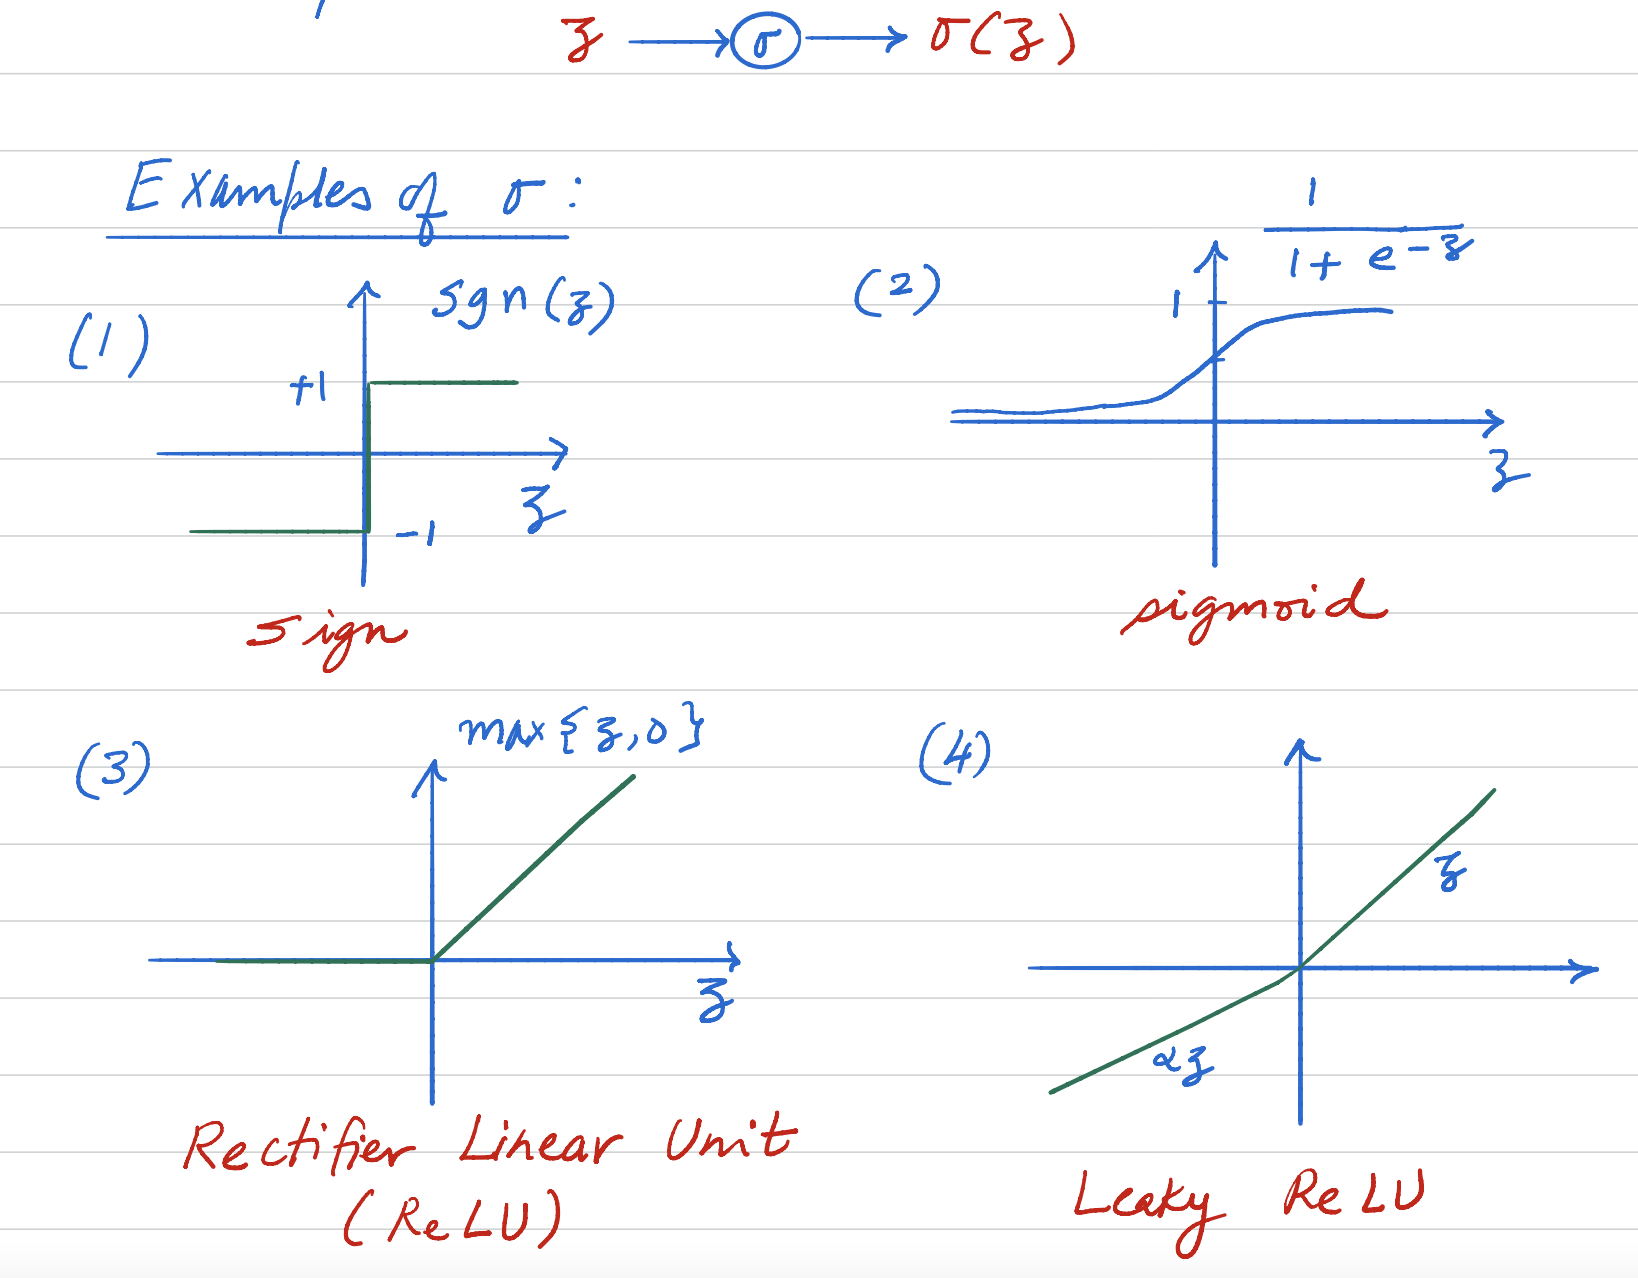
\includegraphics[scale=0.5]{NN.png}
    \caption{Neuron Examples}
    \label{Neuron}
\end{figure}\end{center}

\underline{\textbf{Vector Input}}
\begin{center}\begin{figure}[htbp]
    \centering
    \includegraphics[scale=0.5]{Vector Input}
    \caption{Vector Input}
    \label{}
\end{figure}\end{center}
The output is
\begin{equation}
    \begin{aligned}
        \sigma(\omega^Tx+b)
    \end{aligned}
    \nonumber
\end{equation}


\subsection{Multilayer Neural Network}
\begin{center}\begin{figure}[htbp]
    \centering
    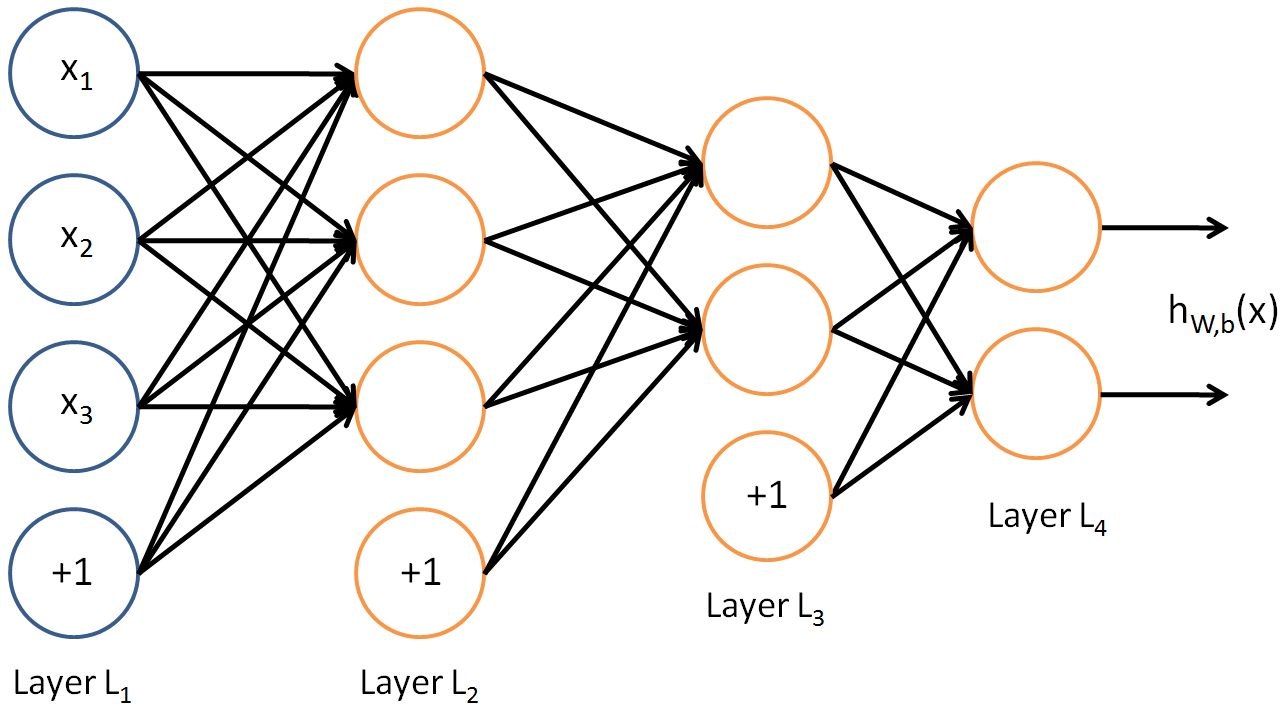
\includegraphics[scale=0.2]{MNN.png}
    \caption{Multilayer Neural Network}
    \label{}
\end{figure}\end{center}
\begin{enumerate}[$\bullet$]
    \item Number of neurons in each layer can be different.
    \item All weights on edge connecting layers $m-1$ and $m$ is matrix $W^{(m)}$, with $w_{ij}^{(m)}$ being the weight connecting output $j$ of layer $m-1$ with neuron $i$ of layer $m$.
    \item Input to network is vector $x$; output of layer $m$ is vector $y^{(m)}$
    \begin{equation}
        \begin{aligned}
            y_i^{(1)}=\sigma(x_i^{(1)}),&\text{ with }x_i^{(1)}=\sum_jw_{ij}^{(1)}x_j+b_i^{(1)}\\
            y^{(1)}=\sigma(x^{(1)}),&\text{ with }x^{(1)}=W^{(1)}x+b^{(1)}\\
            y^{(2)}=\sigma(x^{(2)}),&\text{ with }x^{(2)}=W^{(2)}y^{(1)}+b^{(2)}\\
            \vdots&\\
            y^{(M)}=\sigma(x^{(M)}),&\text{ with }x^{(M)}=W^{(M)}y^{(M-1)}+b^{(M)}\\
        \end{aligned}
        \nonumber
    \end{equation}
\end{enumerate}

We want to find the weights $W^{(1)},\cdots,W^{(M)},b^{(1)},\cdots,b^{(M)}$ so that the output of last layer
\begin{equation}
    \begin{aligned}
        \hat{y}=y^{(M)}\approx f^*(x)=y
    \end{aligned}
    \nonumber
\end{equation}
$f^*(x)$ is the unknown thing we need to predict.

We use \underline{labelled training data}, i.e.
\begin{equation}
    \begin{aligned}
        (x[1],y[1]),(x[2],y[2]),\cdots (x[N],y[N])
    \end{aligned}
    \nonumber
\end{equation}
Minimize the "empirical" loss on training data.
\begin{equation}
    \begin{aligned}
        J=\sum_{i=1}^N L(y[i],\hat{y}[i])
    \end{aligned}
    \nonumber
\end{equation}
where $\bar{y}[i]$ is the output of NN whose input is $x[i]$.

\begin{enumerate}[$\bullet$]
    \item $L$ is the function of $W^{(1)},\cdots,W^{(M)},b^{(1)},\cdots,b^{(M)}$ to measure the loss. e.g. the square loss $$L(y,\hat{y})=(y-\hat{y})^2$$
    \item We wish to minimize $J$ using a \underline{gradient descent procedure}.
    \item To compute gradient we need:
    \begin{equation}
        \begin{aligned}
            \frac{\partial L}{\partial w_{ij}^{(l)}}\text{ for each }l,i,j; \quad
            \frac{\partial L}{\partial b_i^{(l)}}\text{ for each }l,i.\\
        \end{aligned}
        \nonumber
    \end{equation}
\end{enumerate}

\subsection{Back Propagation Algorithm}
Recall $y_i^{(m)}=\sigma(x_i^{(m)})$, $x_i^{(m)}=\sum_jw_{ij}^{(m)}y_j^{(m-1)}+b_i^{(m)}$
\begin{equation}
    \begin{aligned}
        \frac{\partial L}{\partial w_{ij}^{(m)}}=\frac{\partial L}{\partial y_i^{(m)}}\cdot \frac{\partial y_i^{(m)}}{\partial w_{ij}^{(m)}}=\frac{\partial L}{\partial y_i^{(m)}}\cdot \frac{\partial y_i^{(m)}}{\partial x_{i}^{(m)}}\cdot \frac{\partial x_{i}^{(m)}}{\partial w_{ij}^{(m)}}
    \end{aligned}
    \nonumber
\end{equation}
\begin{equation}
    \begin{aligned}
        \frac{\partial L}{\partial b_{i}^{(m)}}&=\frac{\partial L}{\partial y_i^{(m)}}\cdot \frac{\partial y_i^{(m)}}{\partial x_{i}^{(m)}}\cdot \frac{\partial x_{i}^{(m)}}{\partial b_{i}^{(m)}}\\
    \end{aligned}
    \nonumber
\end{equation}

\textbf{\underline{For large $M$}},
\begin{enumerate}[$\bullet$]
    \item $\frac{\partial L}{\partial y_i^{(M)}}$ is easy to compute.
    \item $\frac{\partial y_i^{(M)}}{\partial x_{i}^{(M)}}=\frac{\partial \sigma(x_{i}^{(M)})}{\partial x_{i}^{(M)}}=\sigma'(x_{i}^{(M)})$, (assuming $\sigma$ differentiable).
    \item $\frac{\partial x_{i}^{(M)}}{\partial w_{ij}^{(M)}}=y_j^{(M-1)}$
\end{enumerate}
Thus,
\begin{equation}
    \begin{aligned}
        \frac{\partial L}{\partial w_{ij}^{(M)}}=\frac{\partial L}{\partial y_i^{(M)}}\cdot \sigma'(x_{i}^{(M)}) \cdot y_j^{(M-1)}
    \end{aligned}
    \nonumber
\end{equation}
Similarly,
\begin{equation}
    \begin{aligned}
        \frac{\partial L}{\partial b_{i}^{(M)}}&=\frac{\partial L}{\partial y_i^{(M)}}\cdot \frac{\partial y_i^{(M)}}{\partial x_{i}^{(M)}}\cdot \frac{\partial x_{i}^{(M)}}{\partial b_{i}^{(M)}}\\
        &=\frac{\partial L}{\partial y_i^{(M)}}\cdot \sigma'(x_{i}^{(M)})
    \end{aligned}
    \nonumber
\end{equation}

\textbf{\underline{For $1\leq m< M$}}, in this situation $\frac{\partial L}{\partial y_i^{(m)}}$ is not easy to compute. Note that $x^{(m+1)}=W^{(m+1)}y^{(m)}+b^{(m+1)}$.
\begin{equation}
    \begin{aligned}
    \frac{\partial L}{\partial y_i^{(m)}}&=\sum_k \frac{\partial L}{\partial x_{k}^{(m+1)}}\cdot \frac{\partial x_{k}^{(m+1)}}{\partial y_i^{(m)}}\\
    &=\sum_k \frac{\partial L}{\partial y_{k}^{(m+1)}}\cdot\frac{\partial y_{k}^{(m+1)}}{\partial x_{k}^{(m+1)}}\cdot \frac{\partial x_{k}^{(m+1)}}{\partial y_i^{(m)}}\\
    &=\sum_k \frac{\partial L}{\partial y_{k}^{(m+1)}}\cdot\sigma'(x_k^{(m+1)})\cdot w_{ki}^{(m+1)}\\
    \end{aligned}
    \nonumber
\end{equation}

Then use this form to compute,
\begin{equation}
    \begin{aligned}
        \frac{\partial L}{\partial w_{ij}^{(m)}}&=\frac{\partial L}{\partial y_i^{(m)}}\cdot \frac{\partial y_i^{(m)}}{\partial x_{i}^{(m)}}\cdot \frac{\partial x_{i}^{(m)}}{\partial w_{ij}^{(m)}}\\
        &=\frac{\partial L}{\partial y_i^{(m)}}\cdot \sigma'(x_{i}^{(m)}) \cdot y_j^{(m-1)}
    \end{aligned}
    \nonumber
\end{equation}

Similarly,
\begin{equation}
    \begin{aligned}
        \frac{\partial L}{\partial b_{i}^{(m)}}&=\frac{\partial L}{\partial y_i^{(m)}}\cdot \frac{\partial y_i^{(m)}}{\partial x_{i}^{(m)}}\cdot \frac{\partial x_{i}^{(m)}}{\partial b_{i}^{(m)}}\\
        &=\frac{\partial L}{\partial y_i^{(m)}}\cdot \sigma'(x_{i}^{(m)})
    \end{aligned}
    \nonumber
\end{equation}

\begin{center}
    \fcolorbox{black}{gray!10}{\parbox{.9\linewidth}{
\textbf{Summary}
\begin{enumerate}
    \item Compute $\frac{\partial L}{\partial y_i^{(M)}}$.
    \item Use $$\frac{\partial L}{\partial y_i^{(m)}}=\sum_k \frac{\partial L}{\partial y_{k}^{(m+1)}}\cdot\sigma'(x_k^{(m+1)})\cdot w_{ki}^{(m+1)}$$ compute $\frac{\partial L}{\partial y_i^{(m)}}$ for $m=1,2...,M-1$.
    \item Compute $$\frac{\partial L}{\partial w_{ij}^{(m)}}=\frac{\partial L}{\partial y_i^{(m)}}\cdot \sigma'(x_{i}^{(m)}) \cdot y_j^{(m-1)}$$ for $m=1,2...,M$.
    \item Compute $$\frac{\partial L}{\partial b_{i}^{(m)}}=\frac{\partial L}{\partial y_i^{(m)}}\cdot \sigma'(x_{i}^{(m)})$$ for $m=1,2...,M$.
\end{enumerate}
    }}
\end{center}

\subsection{Other Methods}
Stochastic Gradient Descent (SGD)

Subgradient Method

\section{Constrained Optimization and Gradient Projection}
\subsection{Constrained Optimization: Basic}
\subsubsection{Def: Optimality}
$$\min_{x\in \&} f(x)$$
where $\&$ is a non-empty closed and convex subset of $\mathbb{R}^n$.

Assume $f$ is continuously differentaible on $\&$.

\begin{definition}
$x^*$ is a \underline{local min of $f$ over $\&$} if $\exists \varepsilon>0$ s.t. $f(x^*)\leq f(x)\quad \forall x\in \&$ with $\|x-x^*\|<\varepsilon$.

$x^*$ is \underline{global min of $f$ over $\&$} if $f(x^*)\leq f(x)\quad \forall x\in \&$.
\end{definition}


\subsubsection{Prop: local-min$\Rightarrow\nabla f(x^*)^T(x-x^*)\geq 0,\forall x\in \&$ $\Leftrightarrow$ global-min in convex }
\begin{proposition}[optimality conditions]
    \quad
    \begin{enumerate}[(a)]
        \item (Necessary Conditions for local-min) If $x^*$ is a local min of $f$ over $\&$, then $$\nabla f(x^*)^T(x-x^*)\geq 0\quad \forall x\in \&$$
        \item (Sufficient and Necessary Condition for global-min of convex $f$) If $f$ is convex over $\&$, then above condition is also sufficient for $x^*$ to be a global-min.
    \end{enumerate}
\end{proposition}
\begin{proof}
    \quad
\begin{enumerate}[(a)]
    \item Suppose $x^*$ is a local-min, and $\nabla f(x^*)^T(x-x^*)<0$ for some $x\in \&$.
    
    Let $g(\varepsilon)=f(x^*+\varepsilon(x-x^*))$, then $g'(\varepsilon)=\nabla f(x^*+\varepsilon(x-x^*))^T(x-x^*)$.
    
    By MVT(middle value theorem), $g(\varepsilon)=g(0)+\varepsilon g'(\beta\varepsilon)$ for some $\beta\in[0,1]$
    $$\Rightarrow f(x^*+\varepsilon(x-x^*))=f(x^*)+\varepsilon\nabla f(x^*+\beta\varepsilon(x-x^*))^T(x-x^*)\quad \text{for some }\beta\in[0,1]$$
    Since $\nabla f$ is continuous, we have that for all sufficient small $\varepsilon>0$, $\nabla f(x^*+\beta\varepsilon(x-x^*))^T(x-x^*)<0 \Rightarrow f(x^*+\varepsilon(x-x^*))=f(x^*)$

    Since $x^*+\varepsilon(x-x^*)=\varepsilon x+(1-\varepsilon)x^*\in \&$, then $x^*$ can't be a local-min over $\&$ $\rightarrow$ contradiction.
    \item Convexity of $f$ over $\&$ $\Rightarrow f(x)\geq f(x^*)+\nabla f(x^*)^T(x-x^*),\quad \forall x\in \&$.
    
    Thus,
    \begin{equation}
        \begin{aligned}
            &\nabla f(x^*)^T(x-x^*),\quad \forall x\in \&\\
            \Rightarrow	& f(x)\geq f(x^*)\quad \forall x\in \&\\
            \Rightarrow	& x^*\text{ is a global min of $f$ over }\&
        \end{aligned}
        \nonumber
    \end{equation}
\end{enumerate}
\end{proof}

\subsubsection{Def: Interior Point}
\begin{definition}
    $y$ is an interior point of $\&$ if $\exists \varepsilon>0$ s.t. $$B_{\varepsilon}=\{x:\|y-x\|<\varepsilon\}\subset\&$$
\end{definition}
\underline{Remark:} If $x^*$ is an interior point of $\&$, then
\begin{equation}
    \begin{aligned}
        "x^*\text{ is local min}"&\Rightarrow	"\nabla f(x^*)=0"\\
        \text{If }f\text{ is convex, }"x^*\text{ is global min}"&\Leftrightarrow "\nabla f(x^*)=0"\\
    \end{aligned}
    \nonumber
\end{equation}

\subsection{Constrained Optimization Example}
\begin{align*}
    &\max_{x\in\&}\quad x_1^{a_1}x_2^{a_2}\cdots x_n^{a_n}\\
    &\begin{array}{r@{\quad}r@{}l@{\quad}l}
    &\&=\{x:\sum_{i=1}^nx_i=1,x_i\geq 0,i=1,2,...,n\} &\\
    &a_i,i=1,2,...,n \text{ are given positive scalars}&\\
\end{array} .
\end{align*}
equivalent to $$\min_{x\in\&}\quad f(x)$$ with $f(x)=-\sum a_i\ln x_i$
\begin{equation}
    \begin{aligned}
        \nabla f(x)&=\left(-\frac{a_1}{x_1},-\frac{a_2}{x_2},...,-\frac{a_n}{x_n}\right)\\
        \nabla^2 f(x)&=diag\left(\frac{a_1}{x^2_1},\frac{a_2}{x^2_2},...,\frac{a_n}{x^2_n}\right)\succ 0\\
        &\Rightarrow f\text{ is strictly convex}.
    \end{aligned}
    \nonumber
\end{equation}
\begin{equation}
    \begin{aligned}
        x^*\in\&\text{ is (unique) min}&\Leftrightarrow \nabla f(x^*)^T(x-x^*)\geq 0\quad \forall x\in\&.\\
        &\Leftrightarrow -\sum_{i=1}^n\frac{a_i}{x_i^*}(x-x^*)\geq 0\quad \forall x\in\&.\\
        &\Leftrightarrow -\sum_{i=1}^na_i\frac{x_i}{x_i^*}+\sum_{i=1}^na_i\geq 0\quad \forall x\in\&.\\
    \end{aligned}
    \nonumber
\end{equation}
Guess: $x^*_i=\frac{a_i}{\sum_{i=1}^na_i}$. Then,
\begin{equation}
    \begin{aligned}
        -\sum_{i=1}^n a_i\frac{x_i}{x_i^*}+\sum_{i=1}^na_i=0,\quad \forall x\in\&
    \end{aligned}
    \nonumber
\end{equation}
Thus $x^*=\frac{a_i}{\sum_{i=1}^na_i}$ is unique min.








\subsection{Projection onto Closed Convex Set}
\subsubsection{Def: Projection $[z]^\&$}
\begin{definition}
    Let $\&$ be a \underline{closed convex} subset of $\mathbb{R}^n$. Then, for $z\in \mathbb{R}^n$, the \underline{projection} of $z$ on $\&$ is denoted by $[z]^\&$ and is given by
    $$[z]^\&=\arg \min_{y\in \&}\|z-y\|^2$$
\end{definition}
i.e. Find the min distance from $\&$ to $z$
\begin{center}\begin{figure}[htbp]
    \centering
    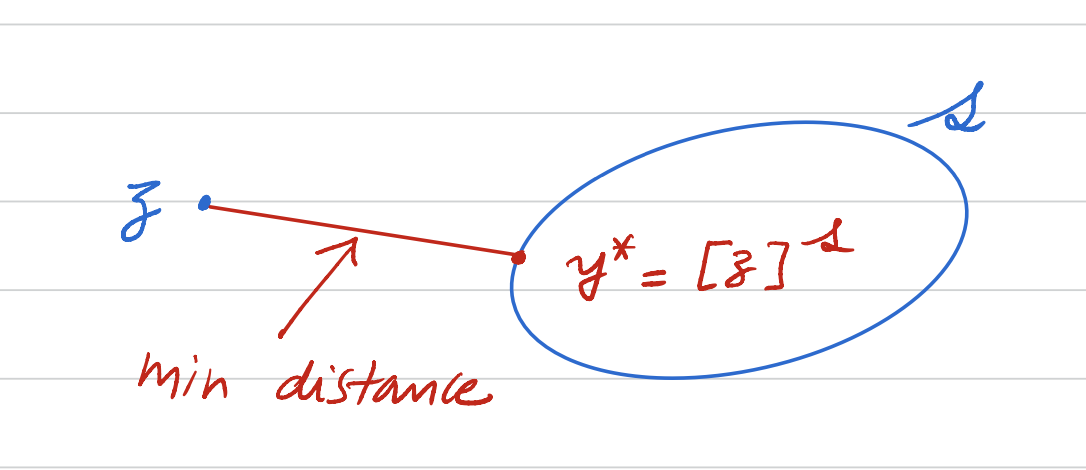
\includegraphics[scale=0.5]{projection1.png}
    \caption{Projection onto Closed Convex Set}
    \label{}
\end{figure}\end{center}
\textbf{Note:} $[z]^\&$ exists and is unique in convex $\&$, however, when $\&$ is not convex, $[z]^\&$ may not be unique.
\begin{center}\begin{figure}[htbp]
    \centering
    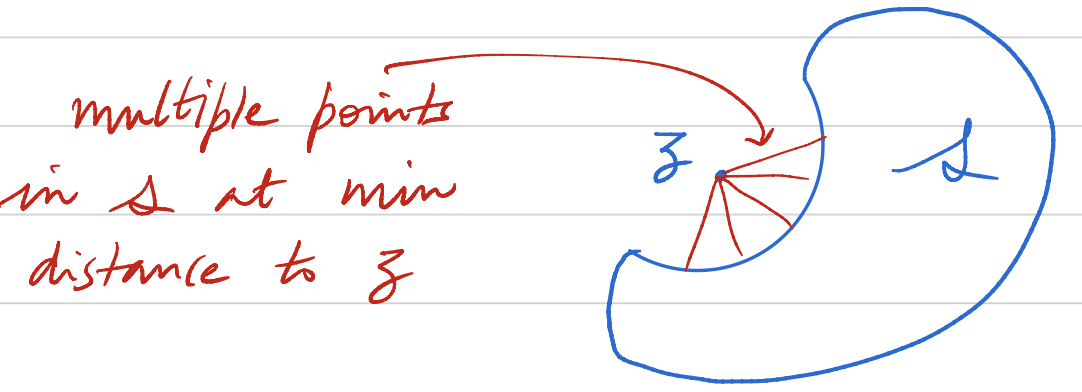
\includegraphics[scale=0.5]{projection2.png}
    \caption{Projection onto Closed non-Convex Set}
    \label{}
\end{figure}\end{center}

\subsubsection{Prop: \underline{unique} projection $[z]^\&$ on \underline{closed convex} subset of $\mathbb{R}^n$}
\begin{proposition}
    [Existence and Uniqueness of Projection]
    Let $\&$ be a \underline{closed convex} subset of $\mathbb{R}^n$. Then, for every $z\in \mathbb{R}^n$, there exists a unique $[z]^\&$.
\end{proposition}
\begin{proof}
Nee to show that $\min_{y\in \&}\|z-y\|^2$ exists and is unique.

Let $x$ be some element of $\&$. Then
\begin{equation}
    \begin{aligned}
        &\text{minimizing $\|z-y\|^2$ over all $y\in\&$}\\
        \equiv&\text{minimizing $\|z-y\|^2$ over the set $A=\{y\in\&:\|z-y\|^2\}$}
    \end{aligned}
    \nonumber
\end{equation}
$g(y)=\|z-y\|^2$ is strictly convex on set $\&$ $\Rightarrow$ $A$ is a convex set and $g$ is convex on $A$.

Also $g$ is continuous $\Rightarrow	A$ is closed.

Finally, $y\in A \Rightarrow \|y\|^2=\|y-z+z\|^2\leq \|y-z\|^2+\|z\|^2\leq \|z-x\|^2+\|z\|^2 \Rightarrow A$ is bounded.

Thus, $g(y)=\|z-y\|^2$ is strictly convex over set $A$, which is compact.

Therefore, $\min_{y\in\&}\|\&-y\|^2=\min_{y\in A}\|\&-y\|^2$ exists (Weierstrass’ Theorem) and is unique (strict convexity).
\end{proof}

\subsubsection{Projection Theorem: $x=[z]^\&$ is projection on \underline{closed conex} subset of $\mathbb{R}^n$$\Leftrightarrow$ $(z-x)^T(y-x)\leq 0, \forall y\in\&$}
\begin{proposition}
    [Necessary and Sufficient Condition for Projection]
    Let $\&$ be a \underline{closed conex} subset of $\mathbb{R}^n$. Then,
    \begin{equation}
        \begin{aligned}
            [z]^\&=y^*
            &\Leftrightarrow (y^*-z)^T(y-y^*)\geq 0,\quad \forall y\in\&.\\
            &\Leftrightarrow (z-y^*)^T(y-y^*)\leq 0,\quad \forall y\in\&.
        \end{aligned}
        \nonumber
    \end{equation}
\end{proposition}
\begin{proof}
    $[z]^\& = \argmin_{y\in\&}g(y)$, with $g(y)=\|z-y\|^2$ (which is strictly convex), $\nabla g(y)=2(y-z)$.

    By the optimality conditions,
    \begin{equation}
        \begin{aligned}
            &y^*\text{ is the unique minimizer of $g(y)$ over $\&$}\\
            \Leftrightarrow	& \nabla g(y^*)^T(y-y^*)\geq 0\quad \forall y\in\&\\
            \Leftrightarrow & (y^*-z)^T(y-y^*)\geq 0,\quad \forall y\in\&.\\
            \Leftrightarrow &(z-y^*)^T(y-y^*)\leq 0,\quad \forall y\in\&.
        \end{aligned}
        \nonumber
    \end{equation}
\end{proof}
\begin{center}\begin{figure}[htbp]
    \centering
    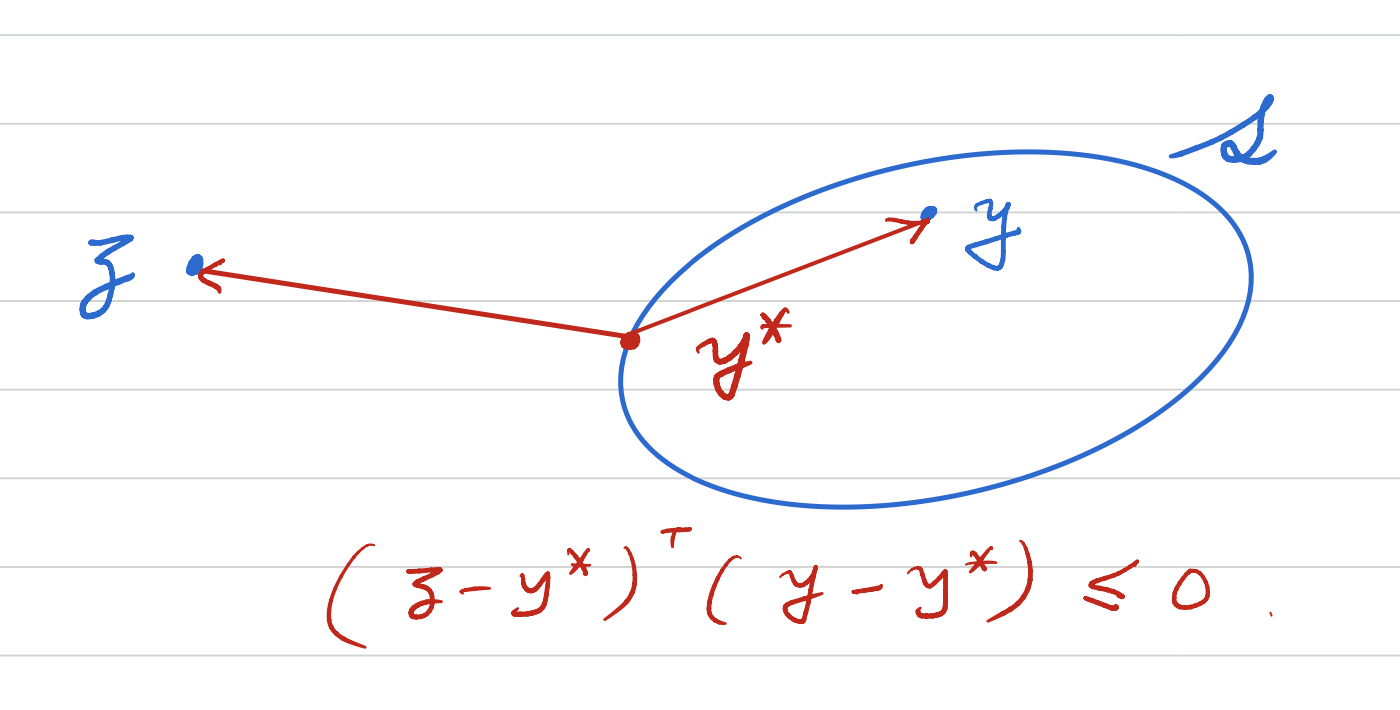
\includegraphics[scale=0.3]{projection3.png}
    \caption{Necessary and Sufficient Condition for Projection}
    \label{}
\end{figure}\end{center}

\subsubsection{Prop: Projection is non-expansive $\|[x]^\&-[z]^\&\|\leq \|x-z\|,\forall x,z\in \mathbb{R}^n$}
\begin{proposition}
    [Projection is non-expansive]
    Let $\&$ be a \underline{closed convex} subset of $\mathbb{R}^n$. Then for $x,z\in \mathbb{R}^n$
    $$\|[x]^\&-[z]^\&\|\leq \|x-z\|\quad \forall x,z\in \mathbb{R}^n$$
\end{proposition}
\begin{proof}
From previous theorem, we know
\begin{equation}
    \begin{aligned}
        (1).\quad ([x]^\&-x)^T(y-[x]^\&)\geq 0,\quad \forall y\in\&.\\
        (2).\quad ([z]^\&-z)^T(y-[z]^\&)\geq 0,\quad \forall y\in\&.\\
    \end{aligned}
    \nonumber
\end{equation}
set $y=[z]^\&$ in (1) and $y=[x]^\&$ in (2), and adding,
\begin{equation}
    \begin{aligned}
        &([z]^\&-[x]^\&)^T([x]^\&-x+z-[z]^\&)\geq 0\\
        \Rightarrow	& ([z]^\&-[x]^\&)^T(z-x)\geq \|[z]^\&-[x]^\&\|^2
    \end{aligned}
    \nonumber
\end{equation}
Applying Cauchy-schwary inequality,
\begin{equation}
    \begin{aligned}
        \|[z]^\&-[x]^\&\|^2&\leq \|[z]^\&-[x]^\&\|\|z-x\|\\
        \|[z]^\&-[x]^\&\|&\leq \|z-x\|
    \end{aligned}
    \nonumber
\end{equation}
\end{proof}

\subsection{Projection on (Linear) Subspaces of $\mathbb{R}^n$}
\subsubsection{Orthogonality Principle in subspaces of $\mathbb{R}^n$: $(z-y^*)^Tx= 0,\forall x\in\&$}
Suppose $\&$ is a linear subspace of $\mathbb{R}^n$, any linear combination of points in $\&$ is also in $\&$. Note that $\&$ is \underline{closed and convex}.

Then, for $z\in \mathbb{R}^n$, $[z]^\&=y^*$ satisfies:
\begin{equation}
    \begin{aligned}
        (z-y^*)^T(y-y^*)\leq 0,\quad \forall y\in\&.
    \end{aligned}
    \nonumber
\end{equation}
According to the property of subsapce, we can infer that
\begin{equation}
    \begin{aligned}
        (z-y^*)^Tx\leq 0,\quad \forall x\in\&.
    \end{aligned}
    \nonumber
\end{equation}
$-x$ also in $\&$, $-x\in\& \Rightarrow$
\begin{equation}
    \begin{aligned}
        (z-y^*)^Tx\geq 0,\quad \forall x\in\&.
    \end{aligned}
    \nonumber
\end{equation}
Then we can infer that
\begin{equation}
    \begin{aligned}
        (z-y^*)^Tx= 0,\quad \forall x\in\&.
    \end{aligned}
    \nonumber
\end{equation}
which is called \underline{orthogonality principle}.

\begin{center}\begin{figure}[htbp]
    \centering
    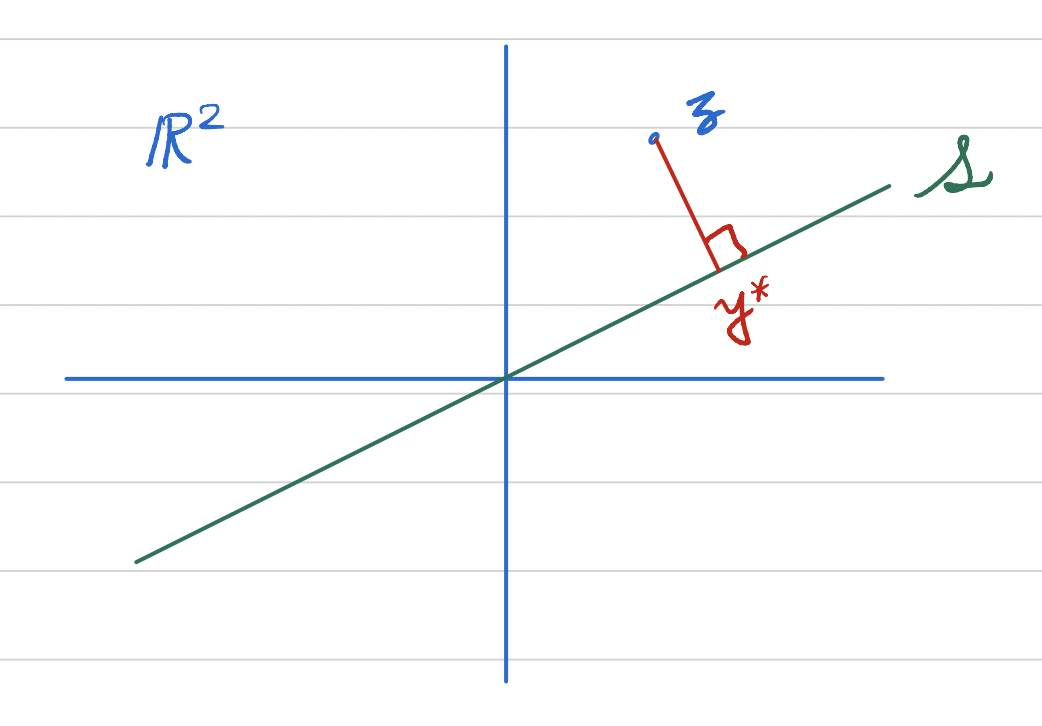
\includegraphics[scale=0.5]{proj1.png}
    \caption{Point from $\mathbb{R}^2$ to $\mathbb{R}$}
    \label{}
\end{figure}\end{center}











\subsection{Gradient Projection Method}
$\min_{x\in\&}f(x)$, $\&$ is convex and closed.
$$x_{k+1}=[x_k+\alpha_k d_k]^\&$$
\underline{Special Case}: Fixed step-size, steepest descent
\begin{equation}
    x_{k+1}=[x_k-\alpha \nabla f(x_k)]^\&
\end{equation}
\subsubsection{Def: \underline{fixed point} in fixed step-size steepest descent method, $\tilde{x}=[\tilde{x}-\alpha \nabla f(\tilde{x})]^\&$}
\begin{definition}
    $\tilde{x}$ is a \underline{fixed (stationary) point} of iteration in (1) if $$\tilde{x}=[\tilde{x}-\alpha \nabla f(\tilde{x})]^\&$$
\end{definition}

\subsubsection{Prop: $L-$smooth, $0<\alpha<\frac{2}{L}$ $\Rightarrow$ limit point is a fixed point (in fixed step-size steepest descent method)}
\begin{proposition}
    If $f$ has $L-$Lipschitz gradient and $0<\alpha<\frac{2}{L}$, every limit point of (1) is a fixed point of (1).
\end{proposition}
\begin{proof}
By the Descent Lemma,
\begin{equation}
    f(x_{k+1})\leq f(x_k)+\nabla f(x_k)^T(x_{k+1}-x_k)+\frac{L}{2}\|x_{k+1}-x_k\|^2
\end{equation}
By the necessary and sufficient condition for projection,
\begin{equation}
    (x_k-\alpha \nabla f(x_k)-x_{k+1})^T(x-x_{k+1})\leq 0,\quad \forall x\in\&
    \nonumber
\end{equation}
Set $x=x_k$ above
\begin{equation}
    \Rightarrow	\alpha \nabla f(x_k)^T(x_{k+1}-x_k)\leq -\|x_k-x_{k+1}\|^2
\end{equation}
According to (2) and (3), $$f(x_{k+1})-f(x_k)\leq (\frac{L}{2}-\frac{1}{\alpha})\|x_k-x_{k+1}\|^2$$ where $\frac{L}{2}-\frac{1}{\alpha}<0$

If $\{x_k\}$ has limit point $\bar{x}$, $LHS \stackrel{k \rightarrow \infty}{\longrightarrow}0$ $$\|x_{k+1}-x_{k}\|\stackrel{k \rightarrow \infty}{\longrightarrow}0 \Rightarrow [\bar{x}-\alpha \nabla f(\bar{x})]^\&=\bar{x}$$
\end{proof}

\subsubsection{Prop: $x$ is minimizer in convex func $\Leftrightarrow$ fixed point (in fixed step-size steepest descent method)}
\begin{proposition}
    If $f$ is convex, then $x^*$ is a minimizer of $f$ over $\&$ $\Leftrightarrow$ $x^*=[x^*-\alpha \nabla f(x^*)]^\&$ (i.e., $x^*$ is a fixed point of (1))
\end{proposition}
\begin{proof}
    \begin{equation}
        \begin{aligned}
            \text{$x^*$ is minimizer of convex $f$ over $\&$} &\Leftrightarrow \nabla f(x^*)^T(x-x^*)\geq 0,\forall x\in \&\\
            &\Leftrightarrow -\alpha\nabla f(x^*)^T(x-x^*)\leq 0,\forall x\in \&\\
            &\Leftrightarrow (x^*-\alpha\nabla f(x^*)-x^*)^T(x-x^*)\leq 0,\forall x\in \&\\
            \text{(By Projection Theorem)}&\Leftrightarrow [x^*-\alpha\nabla f(x^*)]^\&=x^*\\
        \end{aligned}
        \nonumber
    \end{equation}
\end{proof}

\subsubsection{Thm: Convergence of Gradient Projection: Convex, $L-$smooth, $0<\alpha<\frac{2}{L}$ $\Rightarrow$ $f(x_k)\rightarrow f(x^*)$ at rate $\frac{1}{k}$}
\begin{theorem}
    If $f$ is convex and $L-$Lipschitz gradient, it can be shown that for $0<\alpha<\frac{2}{L}$
    $$f(x_k)\rightarrow f(x^*)\text{ at rate }\frac{1}{k}\text{(same as unconstrainted)}$$
\end{theorem}

\subsubsection{Thm: Strongly convex, Lipschitz gradient $\Rightarrow$ $\{x_k\}$ converges to $x^*$ geometrically}
\begin{theorem}
    If $f$ has Lipschitz gradient with Lipschitz constant $M$ and strongly convex with parameter $m$, $\{x_k\}$ converges to $x^*$ \textbf{geometrically}.
\end{theorem}
\begin{proof}
$M-$smooth $\Rightarrow$ $$\|\nabla f(x)-\nabla f(y)\|\leq M\|x-y\|,\quad \forall x,y\in\&$$
$m-$strongly convex $\Rightarrow$
$$\nabla^2 f(x)\succeq mI,\quad \forall x\in\&$$
$$(x-y)^T(\nabla f(x)-\nabla f(y))\geq m\|x-y\|^2\quad \forall x,y\in\&$$
Let $x^*$ be the (unique) min of $f$ over $\&$
\begin{equation}
    \begin{aligned}
        \|x_{k+1}-x^*\|^2&=\|[x_k-\alpha \nabla f(x_k)]^\&-x^*\|^2\\
        (x^*\text{ is fixed point})\quad \quad &=\|[x_k-\alpha \nabla f(x_k)]^\&-[x^*-\alpha \nabla f(x^*)]^\&\|^2\\
        (\text{non-expansive})\quad \quad &\leq \|(x_k-\alpha \nabla f(x_k))-(x^*-\alpha \nabla f(x^*))\|^2\\
        &=\|(x_k-x^*)-\alpha( \nabla f(x_k)- \nabla f(x^*))\|^2\\
        &=\|x_k-x^*\|^2+\alpha^2\|\nabla f(x_k)-\nabla f(x^*)\|^2-2\alpha(x_k-x^*)^T(\nabla f(x_k)-\nabla f(x^*))\\
        (\nabla f\text{ is M-Lipschitz})\quad \quad &\leq \|x_k-x^*\|^2+\alpha^2M^2\|x_k-x^*\|^2-2\alpha(x_k-x^*)^T(\nabla f(x_k)-\nabla f(x^*))\\
        (m-\text{strong convexity})\quad &\leq \|x_k-x^*\|^2+\alpha^2M^2\|x_k-x^*\|^2-2\alpha m\|x_k-x^*\|^2\\
        &=(1+\alpha^2M^2-2\alpha m)\|x_k-x^*\|^2
    \end{aligned}
    \nonumber
\end{equation}
$$\|x_{k+1}-x^*\|^2\leq (1+\alpha^2M^2-2\alpha m)\|x_k-x^*\|^2$$
If $|1+\alpha^2M^2-2\alpha m|<1$. Then $x_N \rightarrow x^*$ \textbf{geometrically} as $N \rightarrow \infty$. (Same as unconstrained case)
\end{proof}



\section{Optimization with Equality Constraints}
\subsection{Basic}
\begin{align*}
    &\min\quad f(x)\\
    &\begin{array}{r@{\quad}r@{}l@{\quad}l}
    s.t.
    &h(x)=0&\\
\end{array}
\end{align*}
where $h(x)=0$ is a combination of $\left\{\begin{matrix}
    h_1(x)=0\\
    h_2(x)=0\\
    \vdots\\
    h_m(x)=0
\end{matrix}\right.$. $f:\mathbb{R}^n \rightarrow \mathbb{R}, h_i:\mathbb{R}^n \rightarrow \mathbb{R}, h:\mathbb{R}^n \rightarrow \mathbb{R}^m$

\underline{Note:} we usually assume 1. $h$ is coninuous, then $H=\{x:h(x)=0\}$ is closed but may not convex; 2. $h_i$ are consistent, i.e., $H$ is non-empty.

\subsection{Lagrange Mutiplier Theorem}
\subsubsection{First-order necessary condition: $\exists\lambda, \nabla f(x^*)+\sum_{i=1}^m\lambda_i \nabla h_i(x^*)=0$}
We say the optimal solution is \underline{regular} if $\nabla h_i(x^*),i=1,...,m$ are linearily independent.
\begin{theorem}[Lagrange Mutiplier Theorem: First-order necessary condition]
    Let $x^*$ be a local-min of $f(x)$ subject to $h(x)=0$. Assume that $\nabla h_i(x^*),i=1,...,m$ are linearily independent. Then $\exists$ a unqiue $\lambda=(\lambda_1,\lambda_2,...,\lambda_m)$ s.t.
    \begin{equation}
        \nabla f(x^*)+\sum_{i=1}^m\lambda_i \nabla h_i(x^*)=0
    \end{equation}
\end{theorem}
Remark: Since $x\in \mathbb{R}^n$, $m=n$ makes the equation trivial. We only consider $m<n$.
\begin{proof}
    Consider sequence of functions:
    \begin{equation}
        \begin{aligned}
            g^{(k)}(x)=f(x)+\frac{k}{2}\|h(x)\|^2+\frac{\alpha}{2}\|x-x^*\|^2,\quad k=1,2,...
        \end{aligned}
        \nonumber
    \end{equation}
    $x^*$ local min of $f(x)$ over $H=\{x:h(x)=0\}$ $\Rightarrow$ $\exists\varepsilon>0$ s.t. $f(x^*)\leq f(x)$ for all $x\in H\cap \&$, where $\&=\{x:\|x-x^*\|\leq \varepsilon\}$.

    According to the Weierstrass's Theorem, $\&\Rightarrow$ Optimal solution to $\min_{x\in\&}g^{(k)}(x)$ exists, we denote the optimal solution to be $x^{(k)}$.
    \begin{lemma}
        $x^{(k)}\rightarrow	x^*$ as $k \rightarrow \infty$
    \end{lemma}
    \begin{proof}
        \begin{equation}
            \begin{aligned}
                g^{(k)}(x^{(k)})&=f(x^{(k)})+\frac{k}{2}\|h(x^{(k)})\|^2+\frac{\alpha}{2}\|x^{(k)}-x^*\|^2,\quad k=1,2,...\\
                &\leq g^{(k)}(x^*)=f(x^*)
            \end{aligned}
            \nonumber
        \end{equation}
    Now since $f(x^{(k)})$ is bounded over $\&$, $\forall k$, we must have $\lim_{k \rightarrow	\infty}\|h(x^{(k)})\|=0$. Thus, every limit point of $x^{(k)}$, $\bar{x}$ must satisfy $h(\bar{x})=0$, i.e., $\bar{x}\in H$.
    \begin{equation}
        \begin{aligned}
            &\Rightarrow	f(\bar{x})+\frac{\alpha}{2}\|\bar{x}-x^*\|^2\leq f(x^*)\\
            (x^*\text{ is local-min, i.e., }f(x^*)\leq f(\bar{x}))\quad &\Rightarrow \bar{x}=x^*
        \end{aligned}
        \nonumber
    \end{equation}
    Thus $\lim_{k \rightarrow\infty}x^{(k)}=x^*$.
    \end{proof}
    According to the lemma, $x^{(k)}$ is an interior point of $\&$ for $k$ sufficiently large.

    $\Rightarrow \nabla g^{(k)}(x^{(k)})=0$ for $k$ sufficiently large.
    \begin{equation}
        \begin{aligned}
            g^{(k)}(x)&=f(x)+\frac{k}{2}\|h(x)\|^2+\frac{\alpha}{2}\|x-x^*\|^2\\
            \nabla g^{(k)}(x)&=\nabla f(x)+k\sum_{i=1}^m h_i(x) \nabla h_i(x)+\alpha(x-x^*)\\
        \end{aligned}
        \nonumber
    \end{equation}
    Let $\nabla h(x)$ denote the combination of $\nabla h_i(x),i=1,...,m$
    \begin{equation}
        \begin{aligned}
            0=&\nabla g^{(k)}(x^{(k)})=\nabla f(x^{(k)})+k\nabla h(x^{(k)})h(x^{(k)})+\alpha(x^{(k)}-x^*)\\
            \Rightarrow	&k\nabla h(x^{(k)})h(x^{(k)})=-(\nabla f(x^{(k)})+\alpha(x^{(k)}-x^*))\\
            \Rightarrow	&kh(x^{(k)})=-\left(\nabla h(x^{(k)})\right)^+(\nabla f(x^{(k)})+\alpha(x^{(k)}-x^*))\\
            \Rightarrow	&\lim_{k \rightarrow \infty}kh(x^{(k)})=-\left(\nabla h(x^{*})\right)^+\nabla f(x^{*})\triangleq \lambda\\
            &\text{(Uniqueness from uniqueness of limit)}
        \end{aligned}
        \nonumber
    \end{equation}
    Where $\left(\nabla h(x^{*})\right)^+$ is the pseudo-inverse of $\nabla h(x^{*})=(\nabla h(x^{*})^T\nabla h(x^{*}))^{-1}\nabla h(x^{*})^T$
    Then
    \begin{equation}
        \begin{aligned}
            \nabla f(x^*)+\sum_{i=1}^m\lambda_i \nabla h_i(x^*)=0
        \end{aligned}
        \nonumber
    \end{equation}
\end{proof}

\subsubsection{Second-order necessary condition: $z^T\left(\nabla^2 f(x^*)+\sum_{i=1}^m\lambda_i \nabla^2 h_i(x^*)\right)z\geq 0,\forall z\in V(x^*)$}
\begin{theorem}
    With the unique $\lambda=(\lambda_1,\lambda_2,...,\lambda_m)$ satisfies $\nabla f(x^*)+\sum_{i=1}^m\lambda_i \nabla h_i(x^*)=0$, the second-order necessary condition is
    \begin{equation}
        \begin{aligned}
            z^T\left(\nabla^2 f(x^*)+\sum_{i=1}^m\lambda_i \nabla^2 h_i(x^*)\right)z\geq 0,\quad \forall z\in V(x^*)
        \end{aligned}
        \nonumber
    \end{equation}
    where $V(x^*)=\{z:\nabla h_i(x^*)^Tz=0,i=1,...,m\}$.
\end{theorem}
\begin{proof}
\begin{equation}
    \begin{aligned}
        \nabla g^{(k)}(x)&=\nabla f(x)+k\sum_{i=1}^m h_i(x) \nabla h_i(x)+\alpha(x-x^*)\\
        \nabla^2 g^{(k)}(x)&=\nabla^2 f(x)+k\sum_{i=1}^m \nabla h_i(x) \nabla h_i(x)^T+k\sum_{i=1}^m h_i(x) \nabla^2 h_i(x)+\alpha I\\
    \end{aligned}
    \nonumber
\end{equation}
Since $x^{(k)}$ is the optimal value of unconstrained minimization of $g^{(k)}(x)$, we have $\nabla^2 g^{(k)}(x^{(k)})\succeq 0$. Then,
\begin{equation}
    \nabla^2 f(x)+k\sum_{i=1}^m \nabla h_i(x) \nabla h_i(x)^T+k\sum_{i=1}^m h_i(x) \nabla^2 h_i(x)+\alpha I\succeq 0
\end{equation}
Consider $z\in V(x^*)=\{z:\nabla h_i(x^*)^Tz=0,i=1,...,m\}$. Let
\begin{equation}
    \begin{aligned}
        z^{(k)}&=z-\nabla h(x^{(k)})\left(\nabla h(x^{(k)})^T\nabla h(x^{(k)})\right)^{-1}\nabla h(x^{(k)})^Tz\\
        &=z-\nabla h(x^{(k)})\left(\nabla h(x^{(k)})\right)^+z
    \end{aligned}
    \nonumber
\end{equation}
Multiply $\nabla h(x^{(k)})$
\begin{equation}
    \begin{aligned}
        \nabla h(x^{(k)})^Tz^{(k)}&=0
    \end{aligned}
    \nonumber
\end{equation}
$(5)$ implies that
\begin{equation}
    \begin{aligned}
        &(z^{(k)})^T\left(\nabla^2 f(x^{(k)})+k\sum_{i=1}^m \nabla h_i(x^{(k)}) \nabla h_i(x^{(k)})^T+k\sum_{i=1}^m h_i(x^{(k)}) \nabla^2 h_i(x^{(k)})+\alpha I\right)z^{(k)}\\
        =&(z^{(k)})^T\left(\nabla^2 f(x^{(k)})+k\sum_{i=1}^m h_i(x^{(k)}) \nabla^2 h_i(x^{(k)})+\alpha I\right)z^{(k)}\geq 0
    \end{aligned}
    \nonumber
\end{equation}
As $k \rightarrow \infty$, $x^{(k)} \rightarrow	x^*$, $kh(x^{(k)})\rightarrow-\left(\nabla h(x^{*})\right)^+\nabla f(x^{*})\triangleq \lambda$ (is proved in first-order necessary condition part), and $z^{(k)}\rightarrow	z$, then
\begin{equation}
    \begin{aligned}
        &z^T\left(\nabla^2 f(x^*)+\sum_{i=1}^m\lambda_i \nabla^2 h_i(x^*)+\alpha I\right)z\geq 0,\quad \forall z\in V(x^*)\\
        &\text{Taking }\alpha \rightarrow 0,\\
        &z^T\left(\nabla^2 f(x^*)+\sum_{i=1}^m\lambda_i \nabla^2 h_i(x^*)\right)z\geq 0,\quad \forall z\in V(x^*)\\
    \end{aligned}
    \nonumber
\end{equation}
\end{proof}

\subsubsection{Sufficient Condition: $\exists\lambda$ 1. $\nabla f(x^*)+\sum_{i=1}^m\lambda_i \nabla h_i(x^*)=0$ 2. $z^T\big(\nabla^2 f(x^*)+\sum_{i=1}^m\lambda_i \nabla^2 h_i(x^*)\big)z> 0,\forall z\in V(x^*),z\neq 0$}
\begin{theorem}
    \underline{Sufficient condition}: For $x^*$ that is feasible and regular, if $\exists \lambda$ s.t.
    \begin{equation}
        \nabla f(x^*)+\sum_{i=1}^m\lambda_i \nabla h_i(x^*)=0
        \nonumber
    \end{equation}
    and
    \begin{equation}
        \begin{aligned}
            z^T\left(\nabla^2 f(x^*)+\sum_{i=1}^m\lambda_i \nabla^2 h_i(x^*)\right)z> 0,\quad \forall z\in V(x^*),z\neq 0
        \end{aligned}
        \nonumber
    \end{equation}
    Then $x^*$ is a (strict) local min for \begin{align*}
        &\min\quad f(x)\\
        &\begin{array}{r@{\quad}r@{}l@{\quad}l}
        s.t.
        &h(x)=0&\\
    \end{array}
    \end{align*}
\end{theorem}
\textbf{Note:}
\begin{enumerate}[(1)]
    \item If $f$ is \underline{convex} and $H=\{x:h(x)=0\}$ is \underline{convex and closed}. Therefore $x^*$ is also global-min.
    \item If $f$ is \underline{coercive} and $H=\{x:h(x)=0\}$ is \underline{closed}. Therefore $f$ can attain its global-min on $\&$, we just find the minimal local-min.
\end{enumerate}


\subsubsection{Lagrangian Function}
\underline{Lagrangian Function}:
\begin{equation}
    \begin{aligned}
        L(x,\lambda)\triangleq f(x)+\sum_{i=1}^m\lambda_i h_i(x)
    \end{aligned}
    \nonumber
\end{equation}
Then the \underline{necessary condition} can be rewrote to
\begin{equation}
    \begin{aligned}
        &\text{First-order:} &
        \left.\begin{matrix}
            \nabla_x L(x^*,\lambda)&=0\\
            h(x^*)=\nabla_\lambda L(x^*,\lambda)&=0
        \end{matrix}\right\}&m+n\text{ equations in total}\\
        &\text{Second-order:} &z^T \nabla_{xx}^2L(x^*,\lambda)z\geq 0,&\quad\forall z\in V(x^*)
    \end{aligned}
    \nonumber
\end{equation}
The \underline{sufficient condition} can be rewrote to
\begin{equation}
    \begin{aligned}
        &\text{First-order:} &
        \nabla_x L(x^*,\lambda)&=0\\
        &\text{Second-order:} &z^T \nabla_{xx}^2L(x^*,\lambda)z&> 0,\quad\forall z\in V(x^*),z\neq 0
    \end{aligned}
    \nonumber
\end{equation}

\subsubsection{Example}
\begin{example}
    \begin{align*}
        &\min\quad \frac{1}{2}(x_1^2+x_2^2+x_3^2)\\
        &\begin{array}{r@{\quad}r@{}l@{\quad}l}
        s.t.
        &x_1+x_2+x_3=3&\\
    \end{array} .
    \end{align*}
\end{example}
\begin{equation}
    \begin{aligned}
        h(x)&=x_1+x_2+x_3-3\\
        L(x,\lambda)&=\frac{1}{2}(x_1^2+x_2^2+x_3^2)+\lambda(x_1+x_2+x_3-3)\\
        \nabla_x L(x,\lambda)&=\left[x_1+\lambda,x_2+\lambda,x_3+\lambda\right]^T\\
        \nabla_{xx}^2 L(x,\lambda)&=I_{3\times 3}\\
    \end{aligned}
    \nonumber
\end{equation}
First order condition:
\begin{equation}
    \begin{aligned}
        \nabla_x L(x^*,\lambda)&=\left[x^*_1+\lambda,x^*_2+\lambda,x^*_3+\lambda\right]^T=0\\
        \Rightarrow	x^*&= [-\lambda,-\lambda,-\lambda]\\
        h(x^*)&=x^*_1+x^*_2+x^*_3-3=0\\
        \Rightarrow	x^*&= [1,1,1]\\
    \end{aligned}
    \nonumber
\end{equation}
And $\nabla_{xx}^2 L(x,\lambda)\succ 0$, then $x^*= [1,1,1]$ is local-min.

\textbf{Note:} Since $f(x)=\frac{1}{2}(x_1^2+x_2^2+x_3^2)$ is coercive on $H=\{x:x_1+x_2+x_3=3\}$ and $H=\{x:x_1+x_2+x_3=3\}$ is closed $\Rightarrow$ $f$ achieves its global min on $H$. $x^*= [1,1,1]$ is the unique local min, so it is also \underline{global-min}.

\subsubsection{Sensitivity Analysis $f(x^*(u))=f(x^*)-\lambda^Tu+O(\|u\|)$}
As constants of constraints change, how will the optimal value change?
\begin{align*}
    &\min\quad f(x)\\
    &\begin{array}{r@{\quad}r@{}l@{\quad}l}
    s.t.
    &h(x)=u&\\
\end{array}
\end{align*}
\begin{claim}
    $$f(x^*(u))=f(x^*)-\lambda^Tu+O(\|u\|)$$
\end{claim}
\begin{proof}
    Let $p(u)=f(x^*(u))$, $p(0)=f(x^*(0))=f(x^*)$

    First-order necessary condition:
    \begin{equation}
        \begin{aligned}
            \nabla f(x^*(u))+\sum_{i=1}^m\lambda_i(u) \nabla h_i(x^*(u))=0\\
            \Rightarrow	\frac{\partial f(x^*(u))}{\partial x_k}=-\sum_{i=1}^m\lambda_i(u) \frac{\partial h_i(x^*(u))}{\partial x_k}
        \nonumber
        \end{aligned}
        \nonumber
    \end{equation}

    \begin{equation}
        \begin{aligned}
            \frac{\partial p(u)}{\partial u_j}=\frac{\partial f(x^*(u))}{\partial u_j}&=\sum_{k=1}^n\frac{\partial f(x^*(u))}{\partial x_k}\frac{\partial x_k^*(u)}{\partial u_j}\\
            &=-\sum_{k=1}^n\sum_{i=1}^m\lambda_i(u) \frac{\partial h_i(x^*(u))}{\partial x_k}\frac{\partial x_k^*(u)}{\partial u_j}\\
            &=-\sum_{i=1}^m\lambda_i(u) \frac{\partial h_i(x^*(u))}{\partial u_j}\\
            (h_i=u_i)\quad &=\lambda_j(u)
        \end{aligned}
        \nonumber
    \end{equation}
Then we can conclude that
\begin{equation}
    \begin{aligned}
        \nabla p(u)&=-\lambda(u)\\
        \Rightarrow	\nabla p(0)&=-\lambda\\
        \Rightarrow	f(x^*(u))&=f(x^*)+\nabla p(0)(u-0)+O(\|u\|)\\
        &=f(x^*)-\lambda^Tu+O(\|u\|)\\
    \end{aligned}
    \nonumber
\end{equation}
\end{proof}

\subsubsection{Linear Constraints}
\begin{align*}
    &\min\quad f(x)\\
    &\begin{array}{r@{\quad}r@{}l@{\quad}l}
    s.t.
    &Ax=b&\\
\end{array}
\end{align*}
where $A=\left[a_1,a_2,...,a_m\right]^T$, $b=[b_1,b_2,...,b_m]^T$. $h_i(x)=a_i^Tx-b_i,i=1,...,m$, $\nabla h_i(x)=a_i$.
\begin{equation}
    \begin{aligned}
        L(x,\lambda)&=f(x)+\sum_{i=1}^m\lambda_i(a_i^Tx-b_i)\\
        \nabla_x L(x,\lambda)&=\nabla f(x)+\sum_{i=1}^m\lambda_ia_i\\
        \nabla^2_{xx} L(x,\lambda)&=\nabla^2 f(x)
    \end{aligned}
    \nonumber
\end{equation}
Then, the first order condition can be reworte to
\begin{equation}
    \begin{aligned}
        &\nabla f(x^*)+\sum_{i=1}^m\lambda_i \nabla h_i(x^*)=0\\
        \Leftrightarrow	&\sum_{i=1}^m\lambda_i a_i=-\nabla f(x^*)\\
        \Leftrightarrow	&A^T\lambda=-\nabla f(x^*)\\
    \end{aligned}
    \nonumber
\end{equation}
Also, $Ax^*=b$. If $m=n$, there will unique $x^*=A^{-1}b$. If $m<n$,
\begin{center}
    \fcolorbox{black}{gray!10}{\parbox{.9\linewidth}{\begin{enumerate}[Step (1)]
        \item We compute first-order condition:
        \begin{equation}
            \begin{aligned}
                \left.\begin{matrix}
                    A^T\lambda+\nabla f(x^*)&=0\\
                    Ax^*&=b
                \end{matrix}\right\}\ m+n\text{ equations}
            \end{aligned}
            \nonumber
        \end{equation}
        \item Check sufficient conditions (second-order):
        Check: $$z^T\nabla^2 f(x)z>0$$ $\forall z\neq 0$ s.t. $a_i^Tz=0,i=1,...,m$
    \end{enumerate}}}
\end{center}

\begin{example}
    \begin{align*}
        &\min\quad -(x_1x_2+x_2x_3+x_1x_3)\\
        &\begin{array}{r@{\quad}r@{}l@{\quad}l}
        s.t.\quad 
        x_1+x_2&=2\\
        x_2+x_3&=1
    \end{array}
    \end{align*}
\end{example}
$A=\begin{bmatrix}
    1&	1&0\\
    0&	1&1
\end{bmatrix}$, $b=\begin{bmatrix}
    2\\
    1
\end{bmatrix}$, $\nabla f(x)=-\begin{bmatrix}
    x_2+x_3\\
    x_1+x_3\\
    x_1+x_2
\end{bmatrix}$

Solve $$\left\{\begin{matrix}
    A^T\lambda+\nabla f(x^*)&=0\\
    Ax^*&=b
\end{matrix}\right. \Rightarrow	x_1^*=2,x_2^*=0,x_3^*=1$$
Check second order condition for $x^*=(2,0,1)$:
\begin{equation}
    \begin{aligned}
        \nabla^2_{xx} L(x,\lambda)&=\nabla^2 f(x)\\
        &=\begin{bmatrix}
            0&-1&-1\\
            -1&0&-1\\
            -1&-1&0
        \end{bmatrix}
    \end{aligned}
    \nonumber
\end{equation}
$\nabla^2_{xx} L(x,\lambda)$ is not PD or PSD. But we only need $z^T\nabla^2 f(x)z>0$ $\forall z\neq 0$ s.t. $a_i^Tz=0,i=1,2$
\begin{equation}
    \begin{aligned}
        Az=\begin{bmatrix}
            z_1+z_2\\
            z_2+z_3
        \end{bmatrix}=0 \Rightarrow	\left\{\begin{matrix}
            z_1=-z_2\\
            z_3=-z_2
        \end{matrix}\right.
    \end{aligned}
    \nonumber
\end{equation}
\begin{equation}
    \begin{aligned}
        z^T\nabla^2 f(x)z&=-2(z_1z_2+z_2z_3+z_1z_3)\\
        &=2z_2^2>0\quad z\neq0
    \end{aligned}
    \nonumber
\end{equation}
Thus $x^*=(2,0,1)$ is a local-min.

\begin{equation}
    \begin{aligned}
        f(x)&=-(x_1x_2+x_2x_3+x_1x_3)\\
        \text{with }h(x)=0\quad &=x_2^2-2
    \end{aligned}
    \nonumber
\end{equation}
$f$ is coercive on $H=\{x:h(x)=0\}$ which is closed. Then $f$ achieves its global min on $H$. Hence, $x^*=(2,0,1)$ is the \underline{global min} of $f(x)$ on $H$.

\section{Optimization with Inequality Constraints}
\subsection{Basic}
Inequality Constraints Problem (ICP)
\begin{align*}
    &\min\quad f(x)\\
    &\begin{array}{r@{\quad}r@{}l@{\quad}l}
    s.t.
    &h(x)=0&\\
    &g(x)\leq 0&\\
\end{array}
\end{align*}
where $h(x)=0$ is a combination of $h_i(x)=0,i=1,...,m$ and $g(x)\leq 0$ is a combination of $g_j(x)\leq 0,j=1,...,r$. $f:\mathbb{R}^n \rightarrow \mathbb{R}, h:\mathbb{R}^n \rightarrow \mathbb{R}^m, g:\mathbb{R}^n \rightarrow \mathbb{R}^r$

\subsubsection{Active vs. Inactive Inequality Constraints}
The constraint $g_j(x)\leq 0$ is said to be \underline{active} at $x$ if $g_j(x)=0$, and \underline{inactive} if $g_j(x)<0$. We set the set of active inequality constraints $A(x)=\{j\in\{1,...,r\}:g_j(x)=0\}$

\subsubsection{ICP $\rightarrow$ ECP}
\underline{Claim}: If $x^*$ is a local min for ICP, then $x^*$ is also a local min for ECP:
\begin{align*}
    &\min\quad f(x)\\
    &\begin{array}{r@{\quad}r@{}l@{\quad}l}
    s.t.
    &h_i(x)=0\quad&i=1,...,m\\
    &g_j(x)= 0\quad&j\in A(x^*)\\
\end{array}
\end{align*}

If $x^*$ is regular for the ECP, i.e., if $\nabla h_i(x^*),i=1,...,m$ and $\nabla g_j(x^*),j=1,...,r$ are linearly independent, then $\exists$ $\lambda_i,i=1,...,m$, $\mu_j,j\in A(x^*)$ s.t.
\begin{equation}
    \begin{aligned}
        \nabla f(x^*)+\sum_{i=1}^m\lambda_i \nabla h_i(x^*)+\sum_{j\in A(x^*)}\mu_j \nabla g_j(x^*)=0
    \end{aligned}
    \nonumber
\end{equation}

\subsubsection{Intuition $\mu_j\geq 0, \forall j\in A(x^*)$}
Consider $g_j(x)\leq 0$ is changed to $g_j(x)\leq u_j$. Then $f(x^*(u_j))\leq f(x^*)$ because of the larger set.

Then, if $j\in A(x^*)$, then $g(x^*)=0$,
\begin{equation}
    \begin{aligned}
        &f(x^*(u_j))=f(x^*)-\mu_ju_j+O(u_j)\\
        \Rightarrow	& -\mu_j u_j+O(u_j)=f(x^*(u_j))-f(x^*)\leq 0
    \end{aligned}
    \nonumber
\end{equation}
Dividing by $u_j$ and letting $u_j \rightarrow 0 \Rightarrow \mu_j\geq 0$

\subsubsection{Complementary Slackness}
\begin{equation}
    \begin{aligned}
        &\mu_j=0\quad \forall j\notin A(x^*)\\
        \Leftrightarrow & \mu_j=0\quad \text{whenever }g_j(x^*)<0, j=1,...,r\\
        \Leftrightarrow & \mu_jg_j(x^*)=0,\quad j=1,...,r
    \end{aligned}
    \nonumber
\end{equation}

\subsection{Karush–Kuhn–Tucker (KKT) Necessary Conditions}
Largrangian Function for ICP:
\begin{equation}
    \begin{aligned}
        L(x,\lambda,\mu)=f(x)+\sum_{i=1}^m\lambda_i h_i(x)+\sum_{j=1}^r\mu_j g_j(x)
    \end{aligned}
    \nonumber
\end{equation}
\begin{proposition}[KKT]
    Let $x^*$ be a \underline{local min of (ICP)} and assume that $x^*$ is regular for (ECP). Then $\exists$ unique largrange multipliers $\lambda=(\lambda_1,...,\lambda_m)$ and $\mu=(\mu_1,...,\mu_r)$ s.t.
    \begin{equation}
        \begin{aligned}
            \nabla_xL(x^*,\lambda,\mu)=0\\
            \mu_j\geq 0,\ j=1,...,r\\
            \mu_j=0,\ \forall j\notin A(x^*)
        \end{aligned}
        \nonumber
    \end{equation}
If $f,h_i,g_j$ are twice continuously differentiable, then $$y^T \nabla^2_{xx}L(x^*,\lambda,\mu)y\geq 0$$
$\forall y\in \mathbb{R}^n$, $\nabla h_i(x^*)^Ty=0,i=1,...,m$, $\nabla g_j(x^*)^Ty=0,\forall j\in A(x^*)$
\end{proposition}

\begin{proof}
Convert (ICP) to:
\begin{align*}
    &\min\quad f(x)\\
    &\begin{array}{r@{\quad}r@{}l@{\quad}l}
    s.t.
    &h_i(x)=0\quad&i=1,...,m\\
    &g_j(x)+z_j^2=0\quad&j=1,...,r\\
\end{array}
\end{align*}
Auxilliary valiables $z=(z_1,...,z_r),z_j\geq 0$.

Let $x^*$ be a local min. For (ICP), then $(x^*,z^*)$ is a local min. $$z_j^*=(-g_j(x^*))^\frac{1}{2},\quad j=1,...,r$$

We can consider the optimization problem over $x$ and $z=(z_1,...,z_r)$. Define Lagrangian:
\begin{equation}
    \begin{aligned}
        L(x,z,\lambda,\mu)=f(x)+\sum_{i=1}^m\lambda_i h_i(x)+\sum_{j=1}^r\mu_j g_j(x)+\sum_{j=1}^r\mu_j z_j^2
    \end{aligned}
    \nonumber
\end{equation}
\begin{enumerate}[(1)]
    \item \underline{First-order necessary condition}
    
    From first-order necessary condition of optimization over $x$ and $z$: assuming $(x^*,z^*)$ is regular,
    \begin{equation}
        \begin{aligned}
            &\nabla L(x^*,z^*,\lambda,\mu)=0\quad \text{Note: $\nabla$ r.t. both $x$ and $z$}\\
            \Rightarrow	&
            \left\{\begin{matrix}
                &\nabla_x f(x^*)+\sum_{i=1}^m \lambda_i \nabla_x h_i(x^*)+\sum_{j=1}^r \mu_j \nabla_x g_j(x^*)=0\\
                &\sum_{j=1}^r \mu_j \nabla_z (z_j^2)|_{z=z^*}=0
            \end{matrix}\right.\\
            \Rightarrow	&
            \left\{\begin{matrix}
                &\nabla_x L(x^*,\lambda,\mu)=0\\
                &\mu_jz_j^*=0,\quad j=1,..,r
            \end{matrix}\right.
        \end{aligned}
        \nonumber
    \end{equation}
    Since $z_j^*=(-g_j(x^*))^{\frac{1}{2}}>0,\forall j\notin A(x^*)$ $\Rightarrow \mu_j=0$ for $j\notin A(x^*)$
    \item \underline{Second-order necessary condition}
    $$\begin{bmatrix}
        y\\
        \omega
    \end{bmatrix}^T \nabla^2L(x^*,z^*,\lambda,\mu)\begin{bmatrix}
        y\\
        \omega
    \end{bmatrix}\geq 0$$
    $\forall y\in \mathbb{R}^n$, $\nabla_x h_i(x^*)^Ty=0,i=1,...,m$, $\nabla_x g_j(x^*)^Ty+2z_j^*\omega_j=0,j=1,...,r$
    \begin{equation}
        \begin{aligned}
            \nabla^2 L(x,z,\lambda,\mu)=\begin{bmatrix}
                \nabla^2_{xx} L(x,\lambda,\mu)&0&0&\cdots&0\\
                0&2\mu_1&0&\cdots&0\\
                0&0&2\mu_2&\cdots&0\\
                \vdots&\ddots&\ddots&\ddots&\vdots\\
                0&\cdots&\cdots&0&2\mu_r
            \end{bmatrix}_{(n+r)\times(n+r)}
        \end{aligned}
        \nonumber
    \end{equation}
    For every $j\in A(x^*)$ select $(y,\omega)$ with $y=0,\omega_j\neq 0$ and $\omega_k=0,\forall k\neq j$.
    
    Then $(y,\omega)$ satisfies $\nabla h_i(x^*)^Ty=0,i=1,...,m$ and $\nabla g_k(x^*)^Ty+2z^*_k\omega_k=0,\forall k\neq j$ and $\nabla g_j(x^*)^Ty+2z_j^*\omega_j=0$ (since $z_j^*=0,\forall j\in A(x^*)$)
    Thus, for the choice of $(y,\omega)$
    \begin{equation}
        \begin{aligned}
            \begin{bmatrix}
                y\\
                \omega
            \end{bmatrix}^T \nabla^2L(x^*,z^*,\lambda,\mu)\begin{bmatrix}
                y\\
                \omega
            \end{bmatrix}=2\mu_j\omega_j^2\geq 0 \Rightarrow \mu_j\geq 0
        \end{aligned}
        \nonumber
    \end{equation}
    Similarly we can show $\mu_j\geq 0,\forall j\in A(x^*)$

    Now choose $y\in \mathbb{R}^n$ s.t. $$\nabla_x h_i(x^*)^T y=0,\quad i=1,...,m,\quad \nabla_x g_j(x^*)^T y=0,\forall j\in A(x^*)$$
    and $\omega$ s.t.
    \begin{equation}
        \begin{aligned}
            \omega_j=\left\{\begin{matrix}
                0&\text{ if }j\in A(x^*)\\
                -\frac{\nabla_x g_j(x^*)^T y}{2z_j^*}&\text{ if }j\notin A(x^*)
            \end{matrix}\right.
        \end{aligned}
        \nonumber
    \end{equation}
    Thus $\nabla_x g_j(x^*)^T y+2z_j^*\omega_j=0\quad \forall j=1,...,r$.
    
    Since $\omega_j=0,\forall j\in A(x^*)$ and $\mu_j=0,\forall j\notin A(x^*)$ $\Rightarrow \mu_j\omega_j=0,\forall j=1,...,r$.

    Then, for the above choive of $(y,\omega)$:
    \begin{equation}
        \begin{aligned}
            \begin{bmatrix}
                y\\
                \omega
            \end{bmatrix}^T \nabla^2L(x^*,z^*,\lambda,\mu)\begin{bmatrix}
                y\\
                \omega
            \end{bmatrix}\geq 0\\
            \Rightarrow	 y^T \nabla^2_{xx}L(x^*,\lambda,\mu)y\geq 0
        \end{aligned}
        \nonumber
    \end{equation}
\end{enumerate}

\end{proof}

\subsection{Karush–Kuhn–Tucker (KKT) Sufficient Conditions}
\begin{proposition}[KKT]
    Suppose $x^*,\lambda,\mu$ satify the first order necessary condition i.e., $\exists$ unique largrange multipliers $\lambda=(\lambda_1,...,\lambda_m)$ and $\mu=(\mu_1,...,\mu_r)$ s.t.
    \begin{equation}
        \begin{aligned}
            \nabla_xL(x^*,\lambda,\mu)=0\\
            \mu_j\geq 0,\ j=1,...,r\\
            \mu_j=0,\ \forall j\notin A(x^*)
        \end{aligned}
        \nonumber
    \end{equation}
    and in addition $$\mu_j {\color{red} >0},\quad \forall j\in A(x^*)$$
    and $$y^T \nabla^2_{xx}L(x^*,\lambda,\mu)y{\color{red} >0}$$
    $\forall y\neq 0$, $\nabla h_i(x^*)^Ty=0,i=1,...,m$, $\nabla g_j(x^*)^Ty=0,\forall j\in A(x^*)$

    Then $x^*$ is a (strict) local min of (ICP).
\end{proposition}
\begin{example}
    \begin{align*}
        &\min\quad 2x_1^2+2x_1x_2+x_2^2-10x_1-10x_2\\
        &\begin{array}{r@{\quad}r@{}l@{\quad}l}
        s.t.
        &x_1^2+x_2^2&\leq 5\\
        &3x_1+x_2&\leq 6\\
    \end{array}
    \end{align*}
\end{example}
\begin{equation}
    \begin{aligned}
        f(x)&=2x_1^2+2x_1x_2+x_2^2-10x_1-10x_2\\
        g_1(x)&=x_1^2+x_2^2-5,\quad g_2(x)=3x_1+x_2-6
    \end{aligned}
    \nonumber
\end{equation}

\begin{equation}
    \begin{aligned}
        \nabla f(x)=\begin{bmatrix}
            4x_1+2x_2-10\\
            2x_1+2x_2-10
        \end{bmatrix}
    \end{aligned},
    \begin{aligned}
        \nabla g_1(x)=\begin{bmatrix}
            2x_1\\
            2x_2
        \end{bmatrix}
    \end{aligned},
    \begin{aligned}
        \nabla g_2(x)=\begin{bmatrix}
            3\\
            1
        \end{bmatrix}
    \end{aligned}
    \nonumber
\end{equation}
\begin{enumerate}[$\bullet$]
    \item \underline{KKT First-order Necessary Condition}: $g_1(x^*)\leq 0$, $g_2(x^*)\leq 0$, assuming $x^*$ regular,
    \begin{equation}
        \begin{aligned}
            \nabla L(x^*,\mu)=\nabla f(x^*)+\mu_1 \nabla g_1(x^*)+\mu_2 \nabla g_2(x^*)=0\\
            \begin{aligned}
                \begin{bmatrix}
                    (4+2\mu_1)x^*_1+2x^*_2+3\mu_2-10\\
                    2x^*_1+(2+2\mu_1)x^*_2+\mu_2-10
                \end{bmatrix}
            \end{aligned}=0\\
            \mu_1\geq 0,\quad \mu_2\geq 0\\
            \mu_1g_1(x^*)=0,\quad \mu_2g_2(x^*)=0\\
            \mu_1((x_1^*)^2+(x_2^*)^2-5)=\mu_2(3x^*_1+x^*_2-6)=0
        \end{aligned}
        \nonumber
    \end{equation}
    We don't know which constraints are active. We \textit{check all possibilities}.
    \begin{enumerate}[(1)]
        \item (1 is inactive, 2 is inactive): $\mu_1=\mu_2=0$ (no need to check for regularity)
        \begin{equation}
            \begin{aligned}
                \nabla f(x)=0 \Rightarrow x_1=0,x_2=5
            \end{aligned}
            \nonumber
        \end{equation}
        which contradicts to $x_1^2+x_2^2\leq 5$.
        \item (1 is inactive, 2 is active), i.e., $\mu_1=0$
        \begin{equation}
            \begin{aligned}
                \begin{aligned}
                    \nabla g_2(x)=\begin{bmatrix}
                        3\\
                        1
                    \end{bmatrix}
                \end{aligned}
            \end{aligned}\Rightarrow \text{ all feasible $x$ are regular}
            \nonumber
        \end{equation}
        \begin{equation}
            \begin{aligned}
                \nabla L(x,\mu)&=\nabla f(x)+\mu_2 \nabla g_2(x)=0\\
                &\Rightarrow \left.\begin{matrix}
                   4x_1+2x_2+3\mu_2-10&=0\\
                   2x_1+2x_2+\mu_2-10&=0\\
                   g_2(x)=0 \Rightarrow 3x_1+x_2-6&=0
                \end{matrix}\right\}\Rightarrow	\left\{\begin{matrix}
                    x_1&=\frac{2}{5}\\
                    x_2&=\frac{24}{5}\\
                    \mu_2&=-\frac{2}{5}
                \end{matrix}\right.
            \end{aligned}
            \nonumber
        \end{equation}
        But $\mu_2<0$ not allowed $\Rightarrow$ solution invalid.
        \item (1 is active, 2 is inactive): $\mu_2=0$
        \begin{equation}
            \begin{aligned}
                \begin{aligned}
                    \nabla g_1(x)=\begin{bmatrix}
                        2x_1\\
                        2x_2
                    \end{bmatrix}
                \end{aligned}
            \end{aligned}\Rightarrow \text{ all $x\neq 0$ are regular}
            \nonumber
        \end{equation}
        \begin{equation}
            \begin{aligned}
                \nabla L(x,\mu)&=\nabla f(x)+\mu_1 \nabla g_1(x)=0\\
                &\Rightarrow \left.\begin{matrix}
                   (4+2\mu_1)x_1+2x_2-10&=0\\
                   2x_1+(2+2\mu_1)x_2-10&=0\\
                   g_1(x)=0 \Rightarrow x_1^2+x_2^2-5&=0
                \end{matrix}\right\}\Rightarrow	\left\{\begin{matrix}
                    x_1&=1\\
                    x_2&=2\\
                  \mu_1&=1
                \end{matrix}\right.
            \end{aligned}
            \nonumber
        \end{equation}
        \underline{check}: $x^*=(1,2)$ is regular (since $\neq 0$)
        \begin{equation}
            \begin{aligned}
                g_1(x^*)=1+4-5=0\\
                g_2(x^*)=3+2-6=-1<0
            \end{aligned}
            \nonumber
        \end{equation}
        Hence, $x^*=(1,2)$, $\mu=(1,0)$ satisfy $1^{st}$ order KKT.
        \item (1 is active, 2 is active)
        
        $\begin{aligned}
            \nabla g_1(x)=\begin{bmatrix}
                2x_1\\
                2x_2
            \end{bmatrix}
        \end{aligned}$ and $\begin{aligned}
            \nabla g_2(x)=\begin{bmatrix}
                3\\
                1
            \end{bmatrix}
        \end{aligned}$ are linearly independent if as $x\neq 0,\ x_1\neq 3x_2$. But $x=0$ doesn't satisfy $g$ But $x=0$ doesn't satisfy either $g_1(x)=0$ or $g_2(x)=0$, and $x_1=3x_2$ can't satisfy $g_1(x)=0,g_2(x)=0$ at the same time. Hence, all feasible $x$ in this case are regular.
        \begin{equation}
            \begin{aligned}
                \nabla L(x,\mu)&=\nabla f(x)+\mu_1 \nabla g_1(x)+\mu_2 \nabla g_2(x)=0\\
                &\Rightarrow \left.\begin{matrix}
                   (4+2\mu_1)x_1+2x_2+3\mu_2-10&=0\\
                   2x_1+(2+2\mu_1)x_2+\mu_2-10&=0\\
                   g_1(x)=0 \Rightarrow x_1^2+x_2^2-5&=0\\
                   g_2(x)=0 \Rightarrow 3x_1+x_2-6&=0
                \end{matrix}\right\}\Rightarrow	\left\{\begin{matrix}
                    x_1&=2.2\\
                    x_2&=-0.5\\
                  \mu_1&=-2.4\\
                  \mu_2&=4.2
                \end{matrix}\right.\text{ or }\left\{\begin{matrix}
                    x_1&=1.4\\
                    x_2&=1.7\\
                  \mu_1&=1.4\\
                  \mu_2&=-1.0
                \end{matrix}\right.
            \end{aligned}
            \nonumber
        \end{equation}
        both not valid since $\mu_1,\mu_2$ are required to be greater than $0$.
    \end{enumerate}
    Hence, the only candidate that satisfies the first order condition is $x^*=(1,2)$, $\mu=(1,0)$
    \item \underline{KKT Second-order Sufficient Condition}:
    $x^*=(1,2)$, $\mu=(1,0)$
    \begin{equation}
        \begin{aligned}
            \nabla^2 L(x^*,\mu)=\begin{bmatrix}
                6&	2\\
                2&	4
            \end{bmatrix}\succ 0
        \end{aligned}
        \nonumber
    \end{equation}
    $\mu_1>0$.

    $\Rightarrow$ $x^*$ is a local min by sufficient condition.
    \item Constraint set: $\&=\{x:g_1(x)\leq 0,g_2\leq 0\}=\{x:x_1^2+x_2^2\leq 5\}\cap \{x:3x_1+x_2\leq 6\}$ which is compact. So, by WT \underline{global minimum} exists which is $x^*=(1,2)$.
\end{enumerate}

\subsection{General Sufficiency Condition}
With possible additional constraints
\begin{align*}
    &\min\quad f(x)\\
    &\begin{array}{r@{\quad}r@{}l@{\quad}l}
    s.t.
    &x\in\&&\leftarrow \text{possible additional constraints}\\
    &h(x)=0&\\
    &g(x)\leq 0&\\
\end{array}
\end{align*}

\begin{theorem}
    Let $L(x,\lambda,\mu)=f(x)+\sum_{i=1}^m\lambda_i h_i(x)+\sum_{j=1}^r\mu_j g_j(x)$.

    Suppose $(x^*,\lambda,\mu)$ satisfy:
    \begin{equation}
        \begin{aligned}
            h_i(x^*)&=0,i=1,...,m\\
            g_j(x^*)&\leq 0,j=1,...,r\\
            \mu_j&\geq 0,j=1,...,r\\
            \mu_jg_j(x^*)&=0,j=1,...,r
        \end{aligned}
        \nonumber
    \end{equation}
    and $$L(x^*,\lambda,\mu)=\min_{x\in\&}L(x,\lambda,\mu)$$
    Then, $x^*$ is a \underline{global min} of this ICP.

    \textbf{Note:} If $\&$ is a \underline{convex} set, and $f$ is \underline{convex}, $h_i$ are affine (linear + constant), $g_j$ are convex over $\&$, then $L(x,\lambda,\mu)$ is convex $\Rightarrow$ $\nabla L(x^*,\lambda,\mu)=0$ is sufficient for $x^*$ to be global min for this ICP.
\end{theorem}



\begin{example}
Application of General Sufficiency Condition of former example:
    \begin{align*}
        &\min_{x\in \mathbb{R}^2}\quad 2x_1^2+2x_1x_2+x_2^2-10x_1-10x_2\\
        &\begin{array}{r@{\quad}r@{}l@{\quad}l}
        s.t.
        &x_1^2+x_2^2&\leq 5\\
        &3x_1+x_2&\leq 6\\
    \end{array}
    \end{align*}
\end{example}
\begin{equation}
    \begin{aligned}
        f(x)&=2x_1^2+2x_1x_2+x_2^2-10x_1-10x_2\\
        g_1(x)&=x_1^2+x_2^2-5,\quad g_2(x)=3x_1+x_2-6
    \end{aligned}
    \nonumber
\end{equation}
For $x^*=(1,2)$ and $\mu=(1,0)$, $L(x,\mu)=f(x)+g_1(x)$ is convex and $\nabla L(x^*,\mu)=0$
$$\Rightarrow L(x^*,\mu)=\min_{x\in \mathbb{R}^2}L(x,\mu)$$
Then, by genral sufficiency condition, $x^*$ is global min.


\subsection{Barrier Method}
Computationed method to solve inequality constrained problems.
\begin{align*}
    &\min\quad f(x)\\
    &\begin{array}{r@{\quad}r@{}l@{\quad}l}
    s.t.
    &x\in\&&\\
    &g(x)\leq 0&\\
\end{array}
\end{align*}
where $\&$ is closed set.
\subsubsection*{Barrier Function}
$B(x)$ is a function that is continuous and $\rightarrow \infty$ as any $g_j(x) \rightarrow	0$
\begin{example}

    \begin{equation}
        \begin{aligned}
            B(x)&=-\sum_{j=1}^r\ln(-g_j(x))\\
            B(x)&=-\sum_{j=1}^r\frac{1}{g_j(x)}
        \end{aligned}
        \nonumber
    \end{equation}

\end{example}
\textbf{Note:} that if $g_j(x)$ is \underline{convex} for all $j$, then both of these barrier functions are \underline{convex}.

In Barrier Method, choose sequence $\{\varepsilon_k\}$ s.t.
\begin{equation}
    \begin{aligned}
        0<\varepsilon_{k+1}<\varepsilon_k,\quad k=0,1,...
    \end{aligned}
    \nonumber
\end{equation}
and $\varepsilon_k \rightarrow 0$ as $k \rightarrow	\infty$.

Define feasible set $F=\&\cap\{g_j(x)\leq 0,\forall j\}$. Note $F$ is a closed set since $\&$ and $\{g_j(x)\leq 0,\forall j\}$ are closed.

Let $x^{(k)}$ be a solution to
\begin{equation}
    \begin{aligned}
        \min_{x\in F\cap \text{dom}(B)}f(x)+\varepsilon_k B(x)
    \end{aligned}
    \nonumber
\end{equation}
Since $B(x) \rightarrow	\infty$ as one $g_j(x) \rightarrow	0$ which is on the boundary of $F$.

$x^{(k)}$ must be an interior point of $F$
$$\Rightarrow \nabla f(x^{(k)})+\varepsilon_k \nabla B(x^{(k)})=0$$
Therefore, if we have a initial point in the interior of $F$, we can choose step size of any unconstrained GD method to stay in interior of $F$ for all iterations and solve the ICP. (Because barrier function $B(x)$ will prevent us from reaching boundary)

As $k \rightarrow \infty$, $\varepsilon_k \rightarrow 0$, and barrier $\varepsilon_k B(x)$ becomes inconsequential, and we expect $x^{(k)}$ to approcah minimum of original problem.

\begin{proposition}
    Every limit point $\bar{x}$ of $\{x^{(k)}\}$ is a global min of the ICP.
\end{proposition}
\begin{proof}
Let $\bar{x}=\lim_{k \rightarrow \infty, k\in \mathcal{K}}x^{(k)}$, since $x^{(k)}\in F$ forall $k$, and $F$ is closed, $\bar{x}\in F$.

Suppose $x^*$ is a global min of ICP and $x^*$ is in interior of $F$, and $f(x^*)<f(\bar{x})$, i.e., $\bar{x}$ is not global min for ICP.

Then, by definition of $x^{(k)}$, $f(x^{(k)})+\varepsilon_k B(x^{(k)})\leq f(x^*)+\varepsilon_k B(x^*)$

Taking limit as $k \rightarrow \infty$, $k\in \mathcal{K}$,
\begin{equation}
    \begin{aligned}
        f(\bar{x})+\lim_{k \rightarrow \infty, k\in \mathcal{K}}\varepsilon_k B(\bar{x})\leq f(x^*)+\lim_{k \rightarrow \infty, k\in \mathcal{K}}\varepsilon_k B(x^*)=f(x^*)\\
        (\text{Since }|B(x^*)|<\infty,\varepsilon_k \rightarrow	0\text{ as }k \rightarrow \infty)
    \end{aligned}
    \nonumber
\end{equation}
If $\bar{x}$ is in interior of $F$, then $|B(\bar{x})|<\infty$ $\Rightarrow \lim_{k \rightarrow \infty, k\in \mathcal{K}}\varepsilon_k B(x^{(k)})=0$

If $\bar{x}$ is on boundary of $F$, then $|B(\bar{x})| \rightarrow \infty$ $\Rightarrow \lim_{k \rightarrow \infty, k\in \mathcal{K}}\varepsilon_k B(x^{(k)})\geq 0$

Therefore, $f(\bar{x})<f(x^*)$ is contradiced.

If $x^*$ is not in interior of $F$, we can assume that $\exists$ an interior point $\bar{x}$ which can be made arbitrarily close to $x^*$.
\end{proof}


\subsection{An Exmaple Using KKT or Barrier}
\begin{example}
\begin{equation}
    \begin{aligned}
        \min\quad&f(x)=\frac{1}{2}(x_1^2+x_2^2)\\
        s.t.\ & x_1\geq 2
    \end{aligned}
    \nonumber
\end{equation}
\end{example}
\subsubsection{Solution using KKT conditions}
\begin{equation}
    \begin{aligned}
        g(x)&=-x_1+2\\
        \nabla g(x)&=(-1,0)\quad \text{All feasible $x$ are regular}\\
        \nabla f(x)&=(x_1,x_2)\\
        L(x,\mu)&=f(x)+\mu g(x)\\
        \nabla L(x,\mu)&=\nabla f(x)+\mu \nabla g(x)=(x_1-\mu,x_2)\\
    \end{aligned}
    \nonumber
\end{equation}
\begin{enumerate}[\underline{Case} $1$:]
    \item constraint inactive, i.e., $\mu=0$
    $$\nabla L(x,\mu)=0 \Rightarrow	x=(0,0)$$
    Doesn't satisfy $x_1\geq 2$. This case is infeasible.
    \item constraint active,
    \begin{equation}
        \begin{aligned}
            \nabla L(x,\mu)=0 \Rightarrow x_1-\mu=0,x_2=0\\
            g(x)=0 \Rightarrow x_1=2\\
            \Rightarrow	x^*=(2,0), \mu=2
        \end{aligned}
        \nonumber
    \end{equation}
    It satisfies the first-order KKT condition.
\end{enumerate}
Since $L(x,\mu)$ is strictly convex on $\mathbb{R}^2$, $x^*=(2,0)$ is the global-min.

\subsubsection{Solution using logarithmic barrier}
$B(x)=-\ln(-g(x))=-\ln(x_1-2)$
\begin{equation}
    \begin{aligned}
        \text{Set }G^{(k)}(x)&=f(x)+\varepsilon_kB(x)\\
        &=\frac{1}{2}(x_1^2+x_2^2)-\varepsilon_k\ln(x_1-2)\\
        (G^{(k)}(x)&\text{ is convex in $x$ over }\{x:x>2\})\\
        \nabla G^{(k)}(x)=0 &\Rightarrow\ x_1-\frac{\varepsilon_k}{x_1-2}=0,\ x_2=0\\
        &\Rightarrow\ x^{(k)}=(1+\sqrt{1+\varepsilon_k},0)\\
        \text{as }k \rightarrow	\infty,\varepsilon_k \rightarrow 0&\text{ and }x^{(k)} \rightarrow (2,0)=x^*
    \end{aligned}
    \nonumber
\end{equation}

\subsection{Penalty Method (For ECP)}
Computational method for \underline{equality constraints}.
\begin{equation}
    \begin{aligned}
        \min\quad &f(x)\\
        s.t.\ &x\in \&\\
        &h_i(x)=0,\quad i=1,...,m
    \end{aligned}
    \nonumber
\end{equation}
\subsubsection*{\underline{Algorithm}}
\begin{enumerate}[(1)]
    \item Choose an increasing positive sequence $\{c_k\}$ s.t. $c_k \rightarrow \infty$ as $k \rightarrow \infty$.
    \item Solve for $x^{(k)}$ to:
    \begin{equation}
        \begin{aligned}
            \min_{x\in \&}\quad &f(x)+c_k\|h(x)\|^2\\
            \text{Note: } &\|h(x)\|^2=\sum_{i=1}^m(h_i(x))^2
        \end{aligned}
        \nonumber
    \end{equation}
\end{enumerate}
\begin{proposition}
    Every limit point $\bar{x}$ of $\{x^{(k)}\}$ is a global min of the ECP if $\&$ is closed.
\end{proposition}
\begin{proof}
    Let $\bar{x}=\lim_{k \rightarrow \infty, k\in \mathcal{K}}x^{(k)}$
    \begin{equation}
        \begin{aligned}
            f^*&=\min_{x\in\&,h(x)=0}f(x)=\min_{x\in\&,h(x)=0}f(x)+c_k\|h(x)\|^2\\
            &\geq \min_{x\in\&}f(x)+c_k\|h(x)\|^2\\
            &=f(x^{(k)})+c_k\|h(x^{(k)})\|^2\\
            \Rightarrow	c_k\|h(x^{(k)})\|^2&\leq f^*-f(x^{(k)})
        \end{aligned}
        \nonumber
    \end{equation}
    By continunity of $f$, $\lim_{k \rightarrow \infty, k\in \mathcal{K}}f(x^{(k)})=f(\bar{x})$.

    Thus, as $k \rightarrow	\infty$, $k \rightarrow	\mathcal{K}$, $f^*-f(x^{(k)})=f^*-f(\bar{x})$ which is \underline{finite}.

    Since $c_k \rightarrow \infty$ as $k \rightarrow	\infty$, $k \rightarrow	\mathcal{K}$, $$\lim_{k \rightarrow \infty, k\in \mathcal{K}}\|h(x^{(k)})\|^2=0$$

    By continunity of $h$,
    $$\lim_{k \rightarrow \infty, k\in \mathcal{K}}\|h(x^{(k)})\|^2=\|h(\bar{x})\|^2=0 \Rightarrow	h(\bar{x})=0$$

    Now, since $\&$ is closed, and $x^{(k)}\in \&$ for all $k$, $\bar{x}\in\&$ as well.

    \begin{equation}
        \begin{aligned}
            &f^*-f(x^{(k)})\geq c_k\|h(x^{(k)})\|^2\geq 0\\
            \Rightarrow	& f(\bar{x})=\lim_{k \rightarrow \infty, k\in \mathcal{K}}f(x^{(k)})\leq f^*
        \end{aligned}
        \nonumber
    \end{equation}
    Since $\bar{x}$ is feasible ($\bar{x}\in\&$ and $h(\bar{x})=0$) and $f(\bar{x})\leq f^*$, $\Rightarrow$ $\bar{x}$ is a global min of the ECP.
\end{proof}

\section{Duality}
\begin{align*}
    &\min\quad f(x)\\
    &\begin{array}{r@{\quad}r@{}l@{\quad}l}
    s.t.
    &x\in\&&\\
    &h(x)=0&\\
    &g(x)\leq 0&\\
\end{array}
\end{align*}
\begin{equation}
    \begin{aligned}
        L(x,\lambda,\mu)&=f(x)+\sum_{i=1}^m\lambda_i h_i(x)+\sum_{j=1}^r\mu_j g_j(x)\\
        &=f(x)+\lambda^T h(x)+\mu^T g(x)
    \end{aligned}
    \nonumber
\end{equation}
\subsubsection*{\underline{Dual Function}}
$D(\lambda,\mu)=\min_{x\in\&}L(x,\lambda,\mu)$ on convex set $G=\{(\lambda,\mu):\lambda\in \mathbb{R}^m,\mu_j\geq 0,j=1,...,r\}$
\begin{proposition}
    $D(\lambda,\mu)$ is concave on $G$
\end{proposition}
\begin{proof}
    Let $(\lambda,\mu)$ and $(\tilde{\lambda},\tilde{\mu})\in G$.

    For $\alpha\in[0,1]$,
    \begin{equation}
        \begin{aligned}
            &D(\alpha\lambda+(1-\alpha)\tilde{\lambda},\alpha\mu+(1-\alpha)\tilde{\mu})\\
            =&\min_{x\in\&}f(x)+(\alpha\lambda+(1-\alpha)\tilde{\lambda})^Th(x)+(\alpha\mu+(1-\alpha)\tilde{\mu})^Tg(x)\\
            =&\min_{x\in\&}\alpha [f(x)+\lambda^Th(x)+\mu^Tg(x)]+(1-\alpha)[f(x)+\tilde{\lambda}^Th(x)+\tilde{\mu}^Tg(x)]\\
            \geq& \min_{x\in \&}\alpha [f(x)+\lambda^Th(x)+\mu^Tg(x)]+\min_{x\in \&}(1-\alpha)[f(x)+\tilde{\lambda}^Th(x)+\tilde{\mu}^Tg(x)]\\
            =&\alpha D(\lambda,\mu)+(1-\alpha)D(\tilde{\lambda},\tilde{\mu})
        \end{aligned}
        \nonumber
    \end{equation}
\end{proof}

\subsection{Weak Duality Theorem: $\max_{(\lambda,\mu)\in G}D(\lambda,\mu)\leq \min_{x\in F}f(x)$}
Define the feasibility set $F=\{x:x\in\&,h(x)=0,g(x)\leq 0\}$
\begin{proposition}
    $$\max_{(\lambda,\mu)\in G}D(\lambda,\mu)\leq \min_{x\in F}f(x)$$
\end{proposition}
\begin{proof}
    For $(\lambda,\mu)\in G$, $x\in F$
    $$L(x,\lambda,\mu)=f(x)+\lambda^T h(x)+\mu^T g(x)\leq f(x)$$
    \begin{equation}
        \begin{aligned}
            \Rightarrow	\min_{x\in F}L(x,\lambda,\mu)&\leq f(x),\quad \forall x\in F\\
            \min_{x\in F}L(x,\lambda,\mu)&\leq \min_{x\in F}f(x)=f^*
        \end{aligned}
        \nonumber
    \end{equation}
    Since $F\subseteq \&$,
    \begin{equation}
        \begin{aligned}
            \min_{x\in \&}L(x,\lambda,\mu)&\leq f^*\\
            \text{i.e. }\quad D(\lambda,\mu)&\leq f^*,\quad \forall (\lambda,\mu)\in G\\
            \Rightarrow	\ \max_{(\lambda,\mu)\in G}D(\lambda,\mu)&\leq f^*
        \end{aligned}
        \nonumber
    \end{equation}
\end{proof}


\subsection{Strong Duality Theorem: under some conditions, $\max_{(\lambda,\mu)\in G}D(\lambda,\mu)= \min_{x\in F}f(x)$}
Under some conditions, equality holds, i.e.
\begin{equation}
    \begin{aligned}
        \underbrace{\max_{(\lambda,\mu)\in G}D(\lambda,\mu)}_{\text{dual problem}}=\underbrace{\min_{x\in F}f(x)}_{\text{primal problem}}
    \end{aligned}
    \nonumber
\end{equation}
\begin{proposition}
    Suppose $f$ is \underline{convex}, $h_i$ are \underline{affine}, $g_j$ are \underline{convex}, and \underline{$\&=\mathbb{R}^n$}. If $x^*$ is an optimal solution for primal problem, $x^*$ is regular, and $(\lambda^*,\mu^*)$ are corresponding Largrange multipliers, then strong duality holds and $(\lambda^*,\mu^*)$ maximize $D(\lambda,\mu)$. $$\max_{(\lambda,\mu)\in G}D(\lambda,\mu)=D(\lambda^*,\mu^*)=f(x^*)=\min_{x\in F}f(x)$$
\end{proposition}
\begin{proof}
    Under regularity assumption, using first-order KKT necessary conditions,
    \begin{equation}
        \begin{aligned}
            \nabla_x L(x^*,\lambda^*,\mu^*)&=0\\
            {\mu^*}^Tg(x^*)&=0
        \end{aligned}
        \nonumber
    \end{equation}
    Since $f$ is \underline{convex}, $h_i$ are \underline{affine}, $g_j$ are \underline{convex},\\
    $L(x^*,\lambda^*,\mu^*)$ is convex in $x$. Thus,
    \begin{equation}
        \begin{aligned}
            L(x^*,\lambda^*,\mu^*)&=\min_{x\in \mathbb{R}^n}L(x,\lambda^*,\mu^*)\\
            &\leq \max_{(\lambda,\mu)\in G}\min_{x\in \mathbb{R}^n}L(x,\lambda,\mu)
        \end{aligned}
        \nonumber
    \end{equation}
    Furthermore,
    \begin{equation}
        \begin{aligned}
            L(x^*,\lambda^*,\mu^*)&=f(x^*)+{\lambda^*}^T \underbrace{h(x^*)}_{=0}+\underbrace{{\mu^*}^T g(x^*)}_{=0}\\
            &=f(x^*)\\
            &\geq f(x^*)+\lambda^Th(x^*)+\mu^Tg(x^*)\quad \forall (\lambda,\mu)\in G\\
            &=L(x^*,\lambda,\mu)\quad \forall (\lambda,\mu)\in G\\
            \Rightarrow	\ L(x^*,\lambda^*,\mu^*)&\geq \max_{(\lambda,\mu)\in G}L(x^*,\lambda,\mu)\\
            &\geq \min_{x\in \mathbb{R}^n}\max_{(\lambda,\mu)\in G}L(x,\lambda,\mu)
        \end{aligned}
        \nonumber
    \end{equation}
    Hence,
    \begin{equation}
        \begin{aligned}
            \min_{x\in \mathbb{R}^n}\max_{(\lambda,\mu)\in G}L(x,\lambda,\mu)\leq L(x^*,\lambda^*,\mu^*)\leq \max_{(\lambda,\mu)\in G}\min_{x\in \mathbb{R}^n}L(x,\lambda,\mu)
        \end{aligned}
        \nonumber
    \end{equation}
    \begin{lemma}
        Consider function $g(y,z)$, $y\in \mathbb{Y}$, $z\in \mathbb{Z}$.
        $$\max_{z\in \mathbb{Z}}\min_{y\in \mathbb{Y}}g(y,z)\leq\min_{y\in \mathbb{Y}}\max_{z\in \mathbb{Z}}g(y,z)$$
    \end{lemma}
    \begin{proof}
        Set $f(z)=\min_{y\in \mathbb{Y}}g(y,z)$
        \begin{equation}
            \begin{aligned}
                f(z)&\leq g(y,z)\quad \forall y\in \mathbb{Y}\\
                \Rightarrow \max_{z\in \mathbb{Z}}f(z)&\leq \max_{z\in \mathbb{Z}}g(y,z)\quad \forall y\in \mathbb{Y}\\
                \Rightarrow \max_{z\in \mathbb{Z}}f(z)&\leq \min_{y\in \mathbb{Y}}\max_{z\in \mathbb{Z}}g(y,z)\\
                \Rightarrow	\max_{z\in \mathbb{Z}}\min_{y\in \mathbb{Y}}g(y,z)&\leq\min_{y\in \mathbb{Y}}\max_{z\in \mathbb{Z}}g(y,z)
            \end{aligned}
            \nonumber
        \end{equation}
    \end{proof}
    By the lemma,
    \begin{equation}
        \begin{aligned}
            \min_{x\in \mathbb{R}^n}\max_{(\lambda,\mu)\in G}L(x,\lambda,\mu)= \max_{(\lambda,\mu)\in G}\min_{x\in \mathbb{R}^n}L(x,\lambda,\mu)= L(x^*,\lambda^*,\mu^*)
        \end{aligned}
        \nonumber
    \end{equation}
    \begin{equation}
        \begin{aligned}
            \max_{(\lambda,\mu)\in G}L(x,\lambda,\mu)&=\max_{(\lambda,\mu)\in G} f(x)+\lambda^T h(x)+\mu^T g(x)\\
            &=\left\{\begin{matrix}
                \infty&\text{ if }x\notin F\\
                f(x)&\text{ if }x\in F
            \end{matrix}\right.\\
            \Rightarrow	\min_{x\in \mathbb{R}^n}\max_{(\lambda,\mu)\in G}L(x,\lambda,\mu)&=\min_{x\in F}f(x)
        \end{aligned}
        \nonumber
    \end{equation}
    Also,
    $$\max_{(\lambda,\mu)\in G}\min_{x\in \mathbb{R}^n}L(x,\lambda,\mu)=\max_{(\lambda,\mu)\in G}D(\lambda,\mu)$$
    Hence,
    $$\max_{(\lambda,\mu)\in G}D(\lambda,\mu)=\min_{x\in F}f(x)$$
    Furthermore,
    \begin{equation}
        \begin{aligned}
            \max_{(\lambda,\mu)\in G}D(\lambda,\mu)=L(x^*,\lambda^*,\mu^*)=D(\lambda^*,\mu^*)
        \end{aligned}
        \nonumber
    \end{equation}
    i.e., $(\lambda^*,\mu^*)$ maximize $D(\lambda,\mu)$
\end{proof}

\begin{center}
    \fcolorbox{black}{gray!10}{\parbox{.9\linewidth}{\textbf{Note:} If the optimization problem is a \underline{linear program} and its is feasible, then strong duality holds (always)

    Two ways to prove: 1) Simplex method; 2) Farkas Lemma.}}
\end{center}

\subsubsection{Slater's sufficient condition for strong duality}
\begin{proposition}[Slater's condition]
    If (1) the primal problem is convex (2) it is strictly feasible, that is, there exists $x$ in the relative interior of $\&$ such that $g_j(x)<0,\forall j$ and $h_i(x)=0,\forall i$. Then, strong duality holds.
\end{proposition}

\subsubsection{Example}
We showed that $x^*=(\frac{3}{2},\frac{1}{2})$ is the global min with $\mu^*=(1,0)$ of
\begin{align*}
    &\min\quad x_1^2+x_2^2-4x_1-2x_2+2\\
    &\begin{array}{r@{\quad}r@{}l@{\quad}l}
    s.t.
    &x_1+x_2&\leq 2\\
    &x_1+2x_3&\leq 3\\
\end{array}
\end{align*}
The optimal value $f(x^*)=-\frac{5}{2}$.
What is the dual of the convex program?
\begin{equation}
    \begin{aligned}
        L(x,\mu)&=x_1^2+x_2^2-4x_1-2x_2+2+\mu_1(x_1+x_2-2)+\mu_2(x_1+2x_2-3)\\
        &=x_1^2+x_2^2+(\mu_1+\mu_2-4)x_1+(\mu_1+2\mu_2-2)x_2+2-2\mu_1-3\mu_2
    \end{aligned}
    \nonumber
\end{equation}
$D(\mu)=\min_{x\in \mathbb{R}^2}L(x,\mu)$
\begin{equation}
    \begin{aligned}
        \nabla_x L(x,\mu)=0 \Rightarrow
        \left\{\begin{matrix}
            2x_1+(\mu_1+\mu_2-4)=0\\
            2x_2+(\mu_1+2\mu_2-2)=0
        \end{matrix}\right. \Rightarrow
        \left\{\begin{matrix}
            x_1&=\frac{-(\mu_1+\mu_2-4)}{2}\\
            x_2&=\frac{-(\mu_1+2\mu_2-2)}{2}
        \end{matrix}\right.
    \end{aligned}
    \nonumber
\end{equation}
\begin{equation}
    \begin{aligned}
        D(\mu)=-\left(\frac{\mu_1+\mu_2-4}{2}\right)^2-\left(\frac{\mu_1+2\mu_2-2}{2}\right)^2+2-2\mu_1-3\mu_2
    \end{aligned}
    \nonumber
\end{equation}

\underline{Dual Problem}
\begin{equation}
    \begin{aligned}
        \max_{\mu_1\geq 0,\mu_2\geq 0}\quad D(\mu)
    \end{aligned}
    \nonumber
\end{equation}
\begin{equation}
    \begin{aligned}
        \nabla D(\mu)=\begin{bmatrix}
            -\mu_1-\frac{3}{2}\mu_2+1\\
            -\frac{3}{2}\mu_1-\frac{5}{2}\mu_2+1
        \end{bmatrix},
        \nabla^2 D(\mu)=\begin{bmatrix}
            -1&-\frac{3}{2}\\
            -\frac{3}{2}&-\frac{5}{2}
        \end{bmatrix}\prec 0 \Rightarrow D(\mu)\text{ is strictly concave.}
    \end{aligned}
    \nonumber
\end{equation}
We can compute $\mu_1^*=1$, $\mu_2^*=0$ (optimum check is omitted), $D(\mu^*)=-\frac{5}{2}=f(x^*)$.

\subsection{Dual of Linear Program}
\begin{center}
    \fcolorbox{black}{gray!10}{\parbox{.9\linewidth}{LP in "standard" form:\begin{equation}
        \begin{aligned}
            &\min\ c^Tx\\
            &s.t.\quad Ax\leq b,x\geq 0
        \end{aligned}
        \nonumber
    \end{equation}}}
\end{center}
\begin{equation}
    \begin{aligned}
        D(\mu_1,\mu_2)
        &=\min_{x\in \mathbb{R}^n}c^Tx+\mu_1^T(Ax-b)-\mu_2^Tx\\
        &=\min_{x\in \mathbb{R}^n}(c^T+\mu_1^TA-\mu_2^T)x-\mu_1^Tb\\
        &=\left\{\begin{matrix}
            -\infty&\text{ if }c^T+\mu_1^TA-\mu_2^T\neq 0\\
            -\mu_1^Tb&\text{ if }c^T+\mu_1^TA-\mu_2^T=0
        \end{matrix}\right.
    \end{aligned}
    \nonumber
\end{equation}
Note: $c^T+\mu_1^TA-\mu_2^T=0 \Leftrightarrow A^T\mu_1+c=\mu_2$

Hence, the dual probelm is:
\begin{equation}
    \begin{aligned}
        &\max_{s.t.\ \mu_1\geq 0,\mu_2\geq 0, A^T\mu_1+c=\mu_2}-\mu_1^Tb\\
        =&\min_{s.t.\ \mu_1\geq 0, A^T\mu_1+c\geq 0}\mu_1^Tb\\
    \end{aligned}
    \nonumber
\end{equation}
\begin{center}
    \fcolorbox{black}{gray!10}{\parbox{.9\linewidth}{Hence, the dual probelm is:\begin{equation}
        \begin{aligned}
            &\min\ \bar{x}^Tb\\
            &s.t.\quad -A^T\bar{x}\leq c,\bar{x}\geq 0
        \end{aligned}
        \nonumber
    \end{equation}}}
\end{center}
It is also easy to show that the dual of dual is exactly the primal.

\textbf{\underline{Note:} when $x$ is not restricted to be positive in primal problem.}
\begin{center}
    \fcolorbox{black}{gray!10}{\parbox{.9\linewidth}{LP in "standard" form:\begin{equation}
        \begin{aligned}
            &\min\ c^Tx\\
            &s.t.\quad Ax\leq b
        \end{aligned}
        \nonumber
    \end{equation}}}
\end{center}
\begin{equation}
    \begin{aligned}
        D(\mu_1,\mu_2)
        &=\min_{x\in \mathbb{R}^n}c^Tx+\mu^T(Ax-b)\\
        &=\min_{x\in \mathbb{R}^n}(c^T+\mu^TA)x-\mu^Tb\\
        &=\left\{\begin{matrix}
            -\infty&\text{ if }c^T+\mu^TA\neq 0\\
            -\mu^Tb&\text{ if }c^T+\mu^TA=0
        \end{matrix}\right.
    \end{aligned}
    \nonumber
\end{equation}

Hence, the dual probelm is:
\begin{equation}
    \begin{aligned}
        &\max_{s.t.\ \mu\geq 0, A^T\mu+c=0}-\mu_1^Tb
    \end{aligned}
    \nonumber
\end{equation}
\begin{center}
    \fcolorbox{black}{gray!10}{\parbox{.9\linewidth}{Hence, the dual probelm is:\begin{equation}
        \begin{aligned}
            &\min\ \bar{x}^Tb\\
            &s.t.\quad -A^T\bar{x}= c,\bar{x}\geq 0
        \end{aligned}
        \nonumber
    \end{equation}}}
\end{center}

\section{Augmented Lagrangian Method (adjusted penalty method)}
\subsection{Motivation}
In penalty method, problem becomes \textbf{ill-conditioned} and the optimization becomes super slow if $c_k$ is huge. (${c_k}$ is an increasing positive sequence s.t. $c_k \rightarrow\infty$ as $k\rightarrow\infty$)

\begin{example}
    When we apply penalty method to
    \begin{equation}
        \begin{aligned}
            &\min\ x^TQx\\
            &s.t.\quad Ax=b
        \end{aligned}
        \nonumber
    \end{equation}
    where $Q\succ 0$, $A_{m\times n},m<n$
\end{example}
$$\min\ x^TQx+c_k\|Ax-b\|^2$$
where $\|Ax-b\|^2=(Ax-b)^T(Ax-b)=x^TA^TAx-2x^TA^Tb+b^Tb$
Note: $A^TA\succeq 0$. Since $m<N$, $rank(A^TA)\leq m<n$ $\Rightarrow$ $\lambda_{\min}(A^TA)=0$

Consider the problem $(P_k)$ corresponding to $c_k$
$$\min\ x^TQx+c_k(x^TA^TAx-2x^TA^Tb+b^Tb)$$
i.e. $$\min\ x^T(Q+c_kA^TA)x-2c_kx^TA^Tb+c_kb^Tb$$
Since $Q\succ 0,c_k>0,A^TA\succeq 0$, $(Q+c_kA^TA)\succ 0$. Hence, $(P_k)$ is stricetly convex optimization problem $\Rightarrow$
\begin{equation}
    \begin{aligned}
        x^{(k)}=\left(\frac{Q}{c_k}+A^TA\right)^{-1}A^Tb
    \end{aligned}
    \nonumber
\end{equation}
If we use gradient descent to solve $(P_k)$, the rate of convergence depends on $$\textbf{condition number} =\frac{\lambda_{\max}\left(\frac{Q}{c_k}+A^TA\right)}{\lambda_{\min}\left(\frac{Q}{c_k}+A^TA\right)}$$
As $c_k \rightarrow \infty$,
\begin{equation}
    \begin{aligned}
        \lambda_{\min}\left(\frac{Q}{c_k}+A^TA\right)\approx \lambda_{\min}\left(A^TA\right)=0
    \end{aligned}
    \nonumber
\end{equation}
i.e. optimization probelm $(P_k)$ becomes ill-conditioned as $k \rightarrow	\infty$

\subsection{Augemented Lagrangian Method}
$$L_c(x,\lambda)=f(x)+\lambda^Th(x)+c\|h(x)\|^2$$
with $\lambda\in \mathbb{R}^n$, $c_k \rightarrow \infty$ as $k \rightarrow\infty$.

If $x^{(k)}\in \argmin_x L_{c_k}(x,\lambda)$, then every limit point $\bar{x}$ of $\{x^{(k)}\}$ is a global min for the $(P)$.

\subsubsection*{What is the advantage of adding $\lambda^Th(x)$?}
If $x^*,\lambda^*$ satisfy the second-order sufficiency condition (for $x^*$ being a strict local min for $(P)$), then $\exists \bar{c}>0$ s.t. \underline{$x^*$ is a local min of $L_c(x,\lambda^*)$} if $c\geq \bar{c}$.

(i.e. for some $\gamma>0$ and $\varepsilon>0$, $L_c(x,\lambda^*)\geq L_c(x^*,\lambda^*)+\frac{\gamma}{2}\|x-x^*\|^2$ for all $x$ s.t. $\|x-x^*\|<\varepsilon$)

Therefore, $(P)$ can be restricted to minimum of $L_c(x,\lambda^*)$ if $c>\bar{c}$. We don't need to discuss the situation that $c \rightarrow \infty$.

Therefore if $\lambda$ can be choosen close to $\lambda^*$, augmented Lagrangian method can work without $c_k \rightarrow\infty$ as $k \rightarrow \infty$. $c_k>\bar{c}$ is enough.

\subsubsection{Method of Multipliers}
Then, the question is \underline{how to make $\lambda$ close to $\lambda^*$ without knowing $\lambda^*$?} \textbf{Duality!}

$$(P):\ \min f(x)\text{ s.t. }h(x)=0$$

\begin{equation}
    \begin{aligned}
        \text{Lagrangian: }& L(x,\lambda)=f(x)+\lambda^Th(x)\\
        \text{Dual: }& D(\lambda)=\min_x L(x,\lambda)
    \end{aligned}
    \nonumber
\end{equation}
Let $x(\lambda)$ be a minimizer of $L(x,\lambda)$. Then $$\nabla_x f(x(\lambda))+\sum_{i=1}^m\lambda_i \nabla_x h_i(x(\lambda))=0$$
and $$D(\lambda)=f(x(\lambda))+\sum_{i=1}^m\lambda_ih(x(\lambda))$$
\begin{equation}
    \begin{aligned}
        \frac{\partial f(x(\lambda))}{\partial \lambda_i}&=\sum_{j=1}^n \frac{\partial f(x(\lambda))}{\partial x_j}\cdot \frac{\partial x_j(\lambda)}{\partial \lambda_i}\\
        &=\left[\frac{\partial x_1(\lambda)}{\partial \lambda_i}\cdots \frac{\partial x_n(\lambda)}{\partial \lambda_i}\right] \nabla_x f(x(\lambda))
    \end{aligned}
    \nonumber
\end{equation}
Define $$\nabla_{\lambda}x(\lambda)=\begin{bmatrix}
    \frac{\partial x_1(\lambda)}{\partial \lambda_1}&\cdots &\frac{\partial x_n(\lambda)}{\partial \lambda_1}\\
    \vdots &\cdots &\vdots\\
    \frac{\partial x_1(\lambda)}{\partial \lambda_m}&\cdots &\frac{\partial x_n(\lambda)}{\partial \lambda_m}
\end{bmatrix}$$
Then $\nabla_{\lambda} f(x(\lambda))=\nabla_\lambda x(\lambda) \nabla_x f(x(\lambda))$, $\nabla_{\lambda} h_i(x(\lambda))=\nabla_{\lambda}x(\lambda)\nabla_xh_i(x(\lambda))$.

\begin{equation}
    \begin{aligned}
        \nabla_{\lambda}D(\lambda)&=\nabla_{\lambda}f(x(\lambda))+\nabla_\lambda\left(\sum_{i=1}^m\lambda_ih(x(\lambda))\right)\\
        &=\nabla_\lambda x(\lambda)\cdot \nabla_x f(x(\lambda))+\sum_{i=1}^m\lambda_i\nabla_{\lambda}x(\lambda)\nabla_xh_i(x(\lambda))+h(x(\lambda))\\
        &=\nabla_\lambda x(\lambda)\underbrace{\left(\nabla_x f(x(\lambda))+\sum_{i=1}^m\lambda_i \nabla_x h_i(x(\lambda))\right)}_{=0\text{ by optimality of }x(\lambda)}+h(x(\lambda))\\
        \Rightarrow	\nabla_{\lambda}D(\lambda)&=h(x(\lambda))
    \end{aligned}
    \nonumber
\end{equation}
$D(\lambda)$ is concave in $\lambda$ $\Rightarrow$ we can use \underline{gradient ascent} to find $\lambda^*$
\begin{equation}
    \begin{aligned}
        \lambda^{(k+1)}&=\lambda^{(k)}+\alpha_k \nabla_\lambda D(\lambda^{(k)})\\
        &=\lambda^{(k)}+\alpha_k h(x(\lambda^{(k)}))
    \end{aligned}
    \nonumber
\end{equation}
This leads to method of multipliers:
\begin{equation}
    \begin{aligned}
        x^{(k)}&\in\argmin_{x}L_{c_k}(x,\lambda^{(k)})\\
        \lambda^{(k+1)}&=\lambda^{(k)}+c_k h(x^{(k)})
    \end{aligned}
    \nonumber
\end{equation}
can show that method of multipliers converges to min of $(P)$ under certain conditions (don't need to take $c_k \rightarrow \infty$)

\subsubsection*{Example:}
\begin{equation}
    \begin{aligned}
        &\min\quad f(x)=\frac{1}{2}(x_1^2+x_2^2)\\
        &s.t.\quad x_1=1
    \end{aligned}
    \nonumber
\end{equation}
Obviously, $x^*=(1,0)$ and $\lambda^*=-1$.
\begin{equation}
    \begin{aligned}
        L_c(x,\lambda)&=\frac{1}{2}(x_1^2+x_2^2)+\lambda(x_1-1)+\frac{c}{2}(x_1-1)^2
    \end{aligned}
    \nonumber
\end{equation}
$x^{(k)}\in\argmin_{x}L_{c_k}(x,\lambda^{(k)})$ $\Rightarrow$ $x^{(k)}\in\argmin_{x}\frac{1}{2}({x_1}^2+{x_2}^2)+\lambda({x_1}-1)+\frac{c_k}{2}({x_1}-1)^2$ $$\Rightarrow x^{(k)}=\left(\frac{c_k-\lambda^{(k)}}{c_k+1},0\right)$$.
\begin{equation}
    \begin{aligned}
        \lambda^{(k+1)}&=\lambda^{(k)}+c_k h(x^{(k)})=\lambda^{(k)}+c_k \left(\frac{c_k-\lambda^{(k)}}{c_k+1}-1\right)
    \end{aligned}
    \nonumber
\end{equation}
$$\Rightarrow \lambda^{(k+1)}=\frac{\lambda^{(k)}}{c_k+1}-\frac{c_k}{c_k+1}$$

\begin{equation}
    \begin{aligned}
        (\lambda^{(k+1)}-\lambda^*)&=\lambda^{(k+1)}+1\\
        &=\frac{\lambda^{(k)}-\lambda^*}{c_k+1}
    \end{aligned}
    \nonumber
\end{equation}
As long as $c_k\geq \bar{c}> 0,\forall \bar{c}>0$, $\lambda^{(k)}\rightarrow \lambda^*$ linearly since $\frac{1}{\bar{c}+1}<1$

Thus $\lambda^{(k)}\rightarrow \lambda^* \Rightarrow x^{(k)} \rightarrow (1,0)=x^*$

\section{Sub-gradient Methods}
Gradient descent methods require $\nabla f$ exists. What if $\nabla f$ doesn't exist at some point?

Recall that when $\nabla f$ exists

$f$ is convex on $\&$ $\Leftrightarrow f(y)\geq f(x)+\nabla f(x)^T(y-x),\forall x,y\in\&$ (the inequality is strict for strict convexity)
\subsection{Sub-gradient}
\begin{definition}
    For \underline{convex} $f$ on $\mathbb{R}^n$, $g$ is called a \textbf{sub-gradient} of $f$ at $x\in \mathbb{R}^n$ if $$f(y)\geq f(x)+g^T(y-x),\quad \forall y\in \mathbb{R}^n$$
\end{definition}
\subsubsection*{\underline{Properties of Sub-gradient}}
\begin{enumerate}[1)]
    \item Sub-gradient always exist at any point for convex functions.
    \item If $\nabla f$ exists at a point $x$ for convex $f$, sub-gradient is \underline{unique and $=\nabla f(x)$}
    \item Some definition for sub-gradient can be applied for non-convex $f$, but sub-gradient may not exist.
\end{enumerate}

\begin{example}
$f(x)=|x|,x\in \mathbb{R}$
\end{example}
For $x\neq 0$, $\nabla f$ exists and $=$ sub-gradient.\\
For $x=0$, any $g\in[-1,1]$ is a sub-gradient.
\begin{proof}\quad
\begin{enumerate}[(1)]
    \item For $y>0$, $f(y)=y\geq f(0)+gy=gy,\forall g\in[-1,1]$
    \item For $y<0$, $f(y)=-y\geq f(0)+gy=gy,\forall g\in[-1,1]$
\end{enumerate}
\end{proof}

\subsection{Sub-differential}
\begin{definition}
    Set of all sub-gradient at $x$ is called \textbf{sub-differential} at $x$, denoted $\partial f(x)$.
\end{definition}
\begin{example}
For $f(x)=|x|$,
\begin{equation}
    \begin{aligned}
        \partial f(x)=\left\{\begin{matrix}
            -1&\text{ if }x<0\\
            [-1,1]&\text{ if }x=0\\
            1&\text{ if }x>0\\
        \end{matrix}\right.
    \end{aligned}
    \nonumber
\end{equation}
\end{example}

\begin{example}
For $f(x)=\max\{1,|x|-1\}$. (Note: $f(x)$ is convex since $1,|x|-1$ are both convex.)
\begin{equation}
    \begin{aligned}
        \partial f(x)=\left\{\begin{matrix}
            -1&\text{ if }x<-2\\
            [-1,0]&\text{ if }x=-2\\
            0&\text{ if }-1<x<2\\
            [0,1]&\text{ if }x=2\\
            1&\text{ if }x>2\\
        \end{matrix}\right.
    \end{aligned}
    \nonumber
\end{equation}
\end{example}
When $x=2$,
\begin{equation}
    \begin{aligned}
        f(y)=\max\{1,|y|-1\}\geq f(2)+g(y-2)=1+g(y-2)
    \end{aligned}
    \nonumber
\end{equation}
\begin{enumerate}[(1)]
    \item \underline{$y\geq 0$}: $0\geq g(y-2)$ or $0\geq (g-1)(y-2)$. If $y>2$, $g\leq 1$; If $y=2$, $\forall g$; If $0\leq y< 2$, $g\geq 0$. $\Rightarrow g\in[0,1]$
    \item \underline{$y< 0$}: $0\geq g(y-2)$ or $-y-2\geq g(y-2)$, i.e. $g\geq 0$ or $g\leq \frac{2+y}{2-y}$ (satisifed by $g\in[0,1]$)
\end{enumerate}

\subsection{More examples}
\begin{example}
    $f(x)=\|x\|=\sqrt{x^Tx}$
\end{example}
\begin{enumerate}[$\bullet$]
    \item $f$ is convex (by Triangle Inequality: $\|x\|+\|y\|\geq \|x+y\|$)
    \item For $x\neq 0$, $\nabla f(x)$ exists and $$\partial f(x)= \nabla f(x) =\frac{1}{2\sqrt{x^Tx}}\cdot 2x=\frac{x}{\|x\|}$$
    \item If $x=0$, $\nabla f(x)$ doesn't exist.
\end{enumerate}
\begin{claim}
    $\partial f(0)=\{g\in \mathbb{R}^n:\|g\|\leq 1\}$
\end{claim}
\begin{proof}
    Need to show that for $\|g\|\leq 1$ and $\forall y\in \mathbb{R}^n$, $$f(y)=\|y\|\geq f(0)+g^T(y-0)=g^T y$$
    But by Cauchy-Schwarz inequality, for $\|g\|\leq 1$, $$g^Ty\leq \|g\|\|y\|\leq \|y\|,\forall y\in \mathbb{R}^n$$
    To estabilish the converse, suppose $\|g\|>1$.

    Then, setting $y=\frac{g}{\|g\|}$ $\Rightarrow$ $\|y\|=1$ but $g^Ty=\|g\|>1=\|y\|$
\end{proof}

\begin{example}
    $f(x)=|x_1-x_2|\leftarrow$ convex
\end{example}
If $x_1>x_2$, $|x_1-x_2|=x_1-x_2$, and $\nabla f$ exists and $(1,-1)$

If $x_1<x_2$, $|x_1-x_2|=x_2-x_1$, and $\nabla f$ exists and $(-1,1)$

\begin{claim}
    If $x_1=x_2$, $\partial f(x)=\{(a,b):a=-b,|a|\leq 1\}$
\end{claim}
\begin{proof}
    Suppose $x_1=x_2=c$. Then we need to show $\forall y\in \mathbb{R}^2$, $(a,b)$ s.t. $a=-b$, $|a|\leq 1$
    \begin{equation}
        \begin{aligned}
            |y_1-y_2|\geq f(c,c)+[a\ b]\begin{bmatrix}
                y_1-c\\
                y_2-c
            \end{bmatrix}=ay_1+by_2-c(a+b)=a(y_1-y_2)
        \end{aligned}
        \nonumber
    \end{equation}
    Since $|a|<1$, this inequality holds $\forall y\in \mathbb{R}^2$
    
    To show the converse,
    \begin{enumerate}
        \item Suppose $a\neq -b$.
        
        If $c(a+b)<0$, setting $y_1=y_2=0$. $\Rightarrow |y_1-y_2|=0$, and $ay_1+by_2-c(a+b)=-c(a+b)>0=|y_1-y_2|$, above inequality fails to hold.

        If $c(a+b)>0$, setting $y_1=y_2=2c$. $\Rightarrow |y_1-y_2|=0$, and $ay_1+by_2-c(a+b)=c(a+b)>0=|y_1-y_2|$, above inequality fails to hold.

        If $c=0$, setting $y_1=y_2=(a+b)$. $\Rightarrow |y_1-y_2|=0$, and $ay_1+by_2-c(a+b)=(a+b)^2>0=|y_1-y_2|$, above inequality fails to hold.
        \item Suppose $a=-b$ with $|a|>1$.
        
        If $a>1$, setting $y_1=y_2+1$; If $a<-1$, setting $y_1=y_2-1$.

    \end{enumerate}
\end{proof}

\subsection{First-order necessary conditions for optimality in terms of subgradient}
\begin{proposition}
    For convex $f$, $f(x^*)=\min_x f(x)\Leftrightarrow 0\in \partial f(x^*)$
\end{proposition}
\begin{proof}
    $x^*$ is a minimizer $\Leftrightarrow$ $f(x^*)\leq f(y),\forall y\in \mathbb{R}^n$ $\Leftrightarrow$ $f(x^*)+0^T(y-x^*)\leq f(y),\forall y\in \mathbb{R}^n$ $\Leftrightarrow$ $0\in \partial f(x^*)$
\end{proof}

\subsection{Properties of Subgradients}
Let $f,f_1,f_2$ be convex functions.
\begin{enumerate}[(a)]
    \item \textbf{Scaling:} For scalar $a > 0$, $\partial(af) = a\partial f$, i.e., $g$ is a subgradient of $f$ at $x$ if and only if $ag$ is a subgradient of af at $x$.
    \item \textbf{Addition:} If $g_1$ is a subgradient of $f_1$ at $x$, and $g_2$ is a subgradient of $f_2$ at $x$, then $g_1 + g_2$ is subgradient of $f_1 + f_2$ at $x$.
    \item \textbf{Affine Combination:} Let $h(x) = f(Ax+b)$, with $A$ being a square, invertible matrix. Then $\partial h(x) = A^T\partial f(Ax+b)$, i.e., $g$ is a subgradient of $f$ at $Ax + b$ if and only if $A^Tg$ is a subgradient of $h$ at $x$.
\end{enumerate}

\subsection{Sub-gradient Descent for Unconstrained Optimization}
\textbf{\underline{Assumptions:}}
\begin{enumerate}[(i)]
    \item $f$ is convex on $\mathbb{R}^n$.
    \item $f^*=\inf_{x\in \mathbb{R}^n}f(x)$ exists and there exists an $x^*$ s.t. $f(x^*)=f^*$.
    \item For all $x\in \mathbb{R}^n$ and for all $g\in \partial f(x)$, $\|g\|\leq a$.
\end{enumerate}
Subgradient Descent with constant step-size:
\begin{equation}
    \begin{aligned}
        x_{k+1}=x_k-\alpha g_k,\quad g_k\in \partial f(x_k)
    \end{aligned}
    \nonumber
\end{equation}
\textbf{\underline{Analysis:}}
\begin{equation}
    \begin{aligned}
        \|x_{k+1}-x^*\|^2&=\|x_k-\alpha g_k-x^*\|^2\\
        &=\|x_k-x^*\|^2+\alpha^2\|g_k\|^2-2\alpha g_k^T(x_k-x^*)\\
        &\leq \|x_k-x^*\|^2+\alpha^2a^2-2\alpha g_k^T(x_k-x^*)
    \end{aligned}
    \nonumber
\end{equation}
By the definition of $g_k$,
\begin{equation}
    \begin{aligned}
        &f(x_k)+g_k^T(x^*-x_k)\leq f(x^*)=f^*
    \end{aligned}
    \nonumber
\end{equation}
\begin{equation}
    \begin{aligned}
        \Rightarrow  \|x_{k+1}-x^*\|^2&\leq \|x_k-x^*\|^2+\alpha^2a^2+2\alpha (f^*-f(x_k))\\
        f(x_k)-f^*&\leq \frac{\|x_k-x^*\|^2-\|x_{k+1}-x^*\|^2+\alpha^2a^2}{2\alpha}
    \end{aligned}
    \nonumber
\end{equation}
Define $f_N^*=\min\{f(x_0),f(x_1),...,f(x_{N-1})\}$
\begin{equation}
    \begin{aligned}
        \sum_{k=0}^{N-1}(f(x_k)-f^*)\geq \sum_{k=0}^{N-1}(f_N^*-f^*)=N(f_N^*-f^*)
    \end{aligned}
    \nonumber
\end{equation}
Then,
\begin{equation}
    \begin{aligned}
        N(f_N^*-f^*)&\leq \sum_{k=0}^{N-1}\frac{\|x_k-x^*\|^2-\|x_{k+1}-x^*\|^2+\alpha^2a^2}{2\alpha}\\
        &=\frac{\|x_0-x^*\|^2-\|x_{N}-x^*\|^2+N\alpha^2a^2}{2\alpha}\\
        \Rightarrow\quad f_N^*&\leq f^*+\frac{1}{2\alpha N}\|x_0-x^*\|^2+\frac{\alpha a^2}{2}\\
        \lim_{N \rightarrow	\infty} f_N^*&\leq f^*+\frac{\alpha a^2}{2}
    \end{aligned}
    \nonumber
\end{equation}
For $\alpha$ samll enough and $N$ large enough $f^*_N$ can be made as close to $f^*$ as desired.

\subsubsection*{Note: $-$subgradient is not necessarily a descent direction}
i.e., if $g_k$ is a subgradient of $f$ at $x_k$. Then $$f(x_k-\alpha g_k)\text{ may be }\geq f(x_k),\quad \forall \alpha>0$$
for some $g_k$.

\begin{example}
    $f(x)=|x_1|+\frac{1}{2}x_2^2$
\end{example}
Suppose $x_k=(0,1)$, then it is easy to show: $\partial f(0,1)=([-1,1],1)$

Consider $g_k=(-1,1)\in\partial f(0,1)$
\begin{equation}
    \begin{aligned}
        f(x_k-\alpha g_k)=f(0+\alpha,1-\alpha)=\frac{1}{2}(1+\alpha^2)>\frac{1}{2}=f(x_k),\forall \alpha>0
    \end{aligned}
    \nonumber
\end{equation}
i.e., $-g_k$ is not a descent direction.

\begin{center}
    \fcolorbox{black}{gray!10}{\parbox{.9\linewidth}{If $f$ is convex, there is some $g_k\in\partial f(x_k)$ for which $-g_k$ is a descent direction (usually the one with \textbf{the smallest norm}), but finding such $g_k$ may be difficult in high-dimentional settings.\\ This means we cannot use back-tracking algorithms (Armijo's Rule) for adopting step-size.}}
\end{center}

\subsection{(Revised) Sub-gradient "descent" with diminishing stepsize}
\textbf{\underline{Assumptions:}}
\begin{enumerate}[(i)]
    \item $f$ is convex on $\mathbb{R}^n$.
    \item $f^*=\inf_{x\in \mathbb{R}^n}f(x)$ exists and there exists an $x^*$ s.t. $f(x^*)=f^*$.
    \item For all $x\in \mathbb{R}^n$ and for all $g\in \partial f(x)$, $\|g\|\leq a$.
\end{enumerate}
Subgradient Descent with constant step-size:
\begin{equation}
    \begin{aligned}
        x_{k+1}=x_k-\alpha_k g_k,\quad g_k\in \partial f(x_k)
    \end{aligned}
    \nonumber
\end{equation}
\textbf{\underline{Analysis:}}
\begin{equation}
    \begin{aligned}
        \|x_{k+1}-x^*\|^2&=\|x_k-\alpha_k g_k-x^*\|^2\\
        &=\|x_k-x^*\|^2+\alpha_k^2\|g_k\|^2-2\alpha_k g_k^T(x_k-x^*)\\
        &\leq \|x_k-x^*\|^2+\alpha_k^2a^2-2\alpha_k g_k^T(x_k-x^*)
    \end{aligned}
    \nonumber
\end{equation}
By the definition of $g_k$,
\begin{equation}
    \begin{aligned}
        &f(x_k)+g_k^T(x^*-x_k)\leq f(x^*)=f^*
    \end{aligned}
    \nonumber
\end{equation}
\begin{equation}
    \begin{aligned}
        \Rightarrow  \|x_{k+1}-x^*\|^2&\leq \|x_k-x^*\|^2+\alpha_k^2a^2+2\alpha_k (f^*-f(x_k))\\
        &\leq \left(\|x_{k-1}-x^*\|^2+\alpha_{k-1}^2a^2+2\alpha_{k-1}(f^*-f(x_{k-1}))\right)+\alpha_k^2a^2+2\alpha_k (f^*-f(x_k))\\
        &\dots\\
        \Rightarrow  \|x_{N}-x^*\|^2&\leq \|x_{0}-x^*\|^2+a^2\sum_{k=0}^{N-1}\alpha_{k}^2+2\sum_{k=0}^{N-1}\alpha_k(f^*-f(x_{k}))
    \end{aligned}
    \nonumber
\end{equation}
Define $f_N^*=\min\{f(x_0),f(x_1),...,f(x_{N-1})\}$
\begin{equation}
    \begin{aligned}
        \|x_{N}-x^*\|^2&\leq \|x_{0}-x^*\|^2+a^2\sum_{k=0}^{N-1}\alpha_{k}^2+2(f^*-f_N^*)\sum_{k=0}^{N-1}\alpha_k
    \end{aligned}
    \nonumber
\end{equation}
Then,
\begin{equation}
    \begin{aligned}
        f_N^*-f^*&\leq \frac{\|x_0-x^*\|^2-\|x_{N}-x^*\|^2+a^2\sum_{k=0}^{N-1}\alpha_k^2}{2\sum_{k=0}^{N-1}\alpha_k}\\
        &\leq \frac{\|x_0-x^*\|^2+a^2\sum_{k=0}^{N-1}\alpha_k^2}{2\sum_{k=0}^{N-1}\alpha_k}
    \end{aligned}
    \nonumber
\end{equation}
Suppse $\{\alpha_k\}$ is such that $\lim_{N \rightarrow	\infty}\frac{\sum_{k=0}^{N-1}\alpha_k^2}{\sum_{k=0}^{N-1}\alpha_k}=0$, then $\lim_{N \rightarrow \infty} f_N^*=f^*$

\subsubsection*{Example of $\{\alpha_k\}$ and convergence rate}
\begin{enumerate}[1)]
    \item $\alpha_k=\frac{1}{k+1},k=0,1,...$
    \begin{equation}
        \begin{aligned}
            &\sum_{k=0}^{N-1}\alpha_k^2=\sum_{k=1}^{N}\frac{1}{k^2}\rightarrow \frac{\pi^2}{6}\\
            &\sum_{k=0}^{N-1}\alpha_k=\sum_{k=1}^{N}\frac{1}{k}>\log N\\
            \Rightarrow&(f^*_N-f^*)\sim O(\frac{1}{\log N})
        \end{aligned}
        \nonumber
    \end{equation}
    \item $\alpha_k=\frac{1}{\sqrt{k+1}},k=0,1,...$
    \begin{equation}
        \begin{aligned}
            &\sum_{k=0}^{N-1}\alpha_k^2=\sum_{k=1}^{N}\frac{1}{k}<\log N+1\\
            &\sum_{k=0}^{N-1}\alpha_k=\sum_{k=1}^{N}\frac{1}{\sqrt{k}}>2\sqrt{N}-2\\
            \Rightarrow&(f^*_N-f^*)\sim O(\frac{\log N}{\sqrt{N}})
        \end{aligned}
        \nonumber
    \end{equation}
\end{enumerate}
Both worse than gradient descent (GD) $O(\frac{1}{N})$.


\section{Statistical Inference}

\subsection{Basics}
Given an observation $x\in X$, we want to estimate an unknown state $\theta \in S$ (not necessarily random). The $\theta$ can form $x$ with $P_\theta(x)$. We use decision rule $\delta (x)$ to form an action (estimation of $\theta$) $a=\hat{\theta}$.

\textbf{Example:}
\begin{enumerate}[(1)]
    \item Binary hypothesis testing (detection) when $S=\{0,1\}$ e.g. $P_0\sim N(0,\sigma^2), P_1\sim N(\mu,\sigma^2)$
    \item Multiple hypothesis testing (classification) when $S=\{1,2,...,n\}$
    \item When $S=\mathbb{R}$ e.g. $P_\theta\in N(\theta,\sigma^2)$
\end{enumerate}

\subsection{Decision Rule}
\subsubsection*{Binary HT Example}
For the example Binary HT, $P_0\sim N(0,\sigma^2), P_1\sim N(\mu,\sigma^2)$: decision rule $\delta: \mathbb{R} \rightarrow \{0,1\}$

We can find a $\tau$ such that $\delta(x)=\left\{\begin{matrix}
    1,&x\ge \tau\\
    0,& else
\end{matrix}\right.=\mathbf{1}_{x\geq \tau}$. Howe to choose $\tau$?

Type-I error probability: probability that $\theta$ is $0$ but receive $\delta(x)=1$. $$P_I=P_0\{\delta(x)=1\}=P_0\{x\geq \tau\}=Q\left(\frac{\tau}{\sigma}\right)$$
Type-II error probability: probability that $\theta$ is $1$ but receive $\delta(x)=0$. $$P_{II}=P_1\{\delta(x)=0\}=P_1(x<\tau)=Q(\frac{\mu-\tau}{\sigma})$$

Both $P_I$ and $P_{II}$ depends on $\tau$. $Q(t)=\int_t^\infty\frac{e^{-\frac{x^2}{2}}}{\sqrt{2\pi}}dx$

For $\tau=\frac{\mu}{2}$, $P_I=P_{II}=Q\left(\frac{\mu}{2\sigma}\right)$

\subsubsection*{Multiple HT Example}
Consider three state $S=\{1,2,3\}$.
We can find a $\tau$ such that $\delta(x)=\left\{\begin{matrix}
    1,&x< \tau_1\\
    2,& \tau_1\leq x\leq \tau_2\\
    3,& x>\tau_2
\end{matrix}\right.=\mathbf{1}_{x\geq \tau}$.

\textit{Conditional Error Probabilities:} probability that $\theta$ is $i$ but receive $\delta(x)=j$ (6 types in this example) $$P_i\{\delta(x)=j\}, \forall i\neq j$$

\subsubsection*{Estimation Example}
Ex: $P_\theta\sim N(\theta,\sigma^2)$. Perform $\delta(x)=\hat{\theta}$ by using mean-squared error (MSE):
$$MSE= \mathbb{E}_\theta \left[(\delta(x)-\theta)^2\right],\theta\in \mathbb{R}$$

\subsubsection{Maximum-Likelihood Principle}
Maximum-Likelihood Principle $$\hat{\theta}=\argmax_{\theta\in S}P_{\theta}(x)=\argmax_{\theta\in S}\ln P_{\theta}(x)$$
Applied to the binary example: $P_0\sim N(0,\sigma^2), P_1\sim N(\mu,\sigma^2)$.

$P_0(x)=\frac{1}{\sqrt{2\pi}\sigma}e^{-\frac{x^2}{2\sigma^2}}, P_1(x)=\frac{1}{\sqrt{2\pi}\sigma}e^{-\frac{(x-\mu)^2}{2\sigma^2}}$. $\ln P_0(x)=c-\frac{x^2}{2\sigma^2}$, $\ln P_1(x)=c-\frac{(x-\mu)^2}{2\sigma^2}$.

Then, the rule can become $$\hat{\theta}=\left\{\begin{matrix}
    0,&x^2<(x-\mu)^2\\
    1,&else
\end{matrix}\right.=\mathbf{1}_{x^2\geq (x-\mu)^2}=\mathbf{1}_{x\geq \frac{\mu}{2}}$$

\subsubsection*{Vector Observations}
Observations $X=\left(x_1,x_2,...,x_n\right)$, where i.i.d. $x_i\sim P_\theta$. Then $$P_\theta(X)=\prod_{i=1}^n P_\theta(x_i),\ \ln P_\theta(X)=\sum_{i=1}^n\ln P_\theta(x_i)$$
$\ln P_0(x)=cn-\frac{\sum_{i=1}^n x_i^2}{2\sigma^2}$, $\ln P_1(x)=cn-\frac{\sum_{i=1}^n(x_i-\mu)^2}{2\sigma^2}$.

Then, the rule can become $$\hat{\theta}=\left\{\begin{matrix}
    0,&\sum_{i=1}^nx_i^2<\sum_{i=1}^n(x_i-\mu)^2\\
    1,&else
\end{matrix}\right.=\mathbf{1}_{\sum_{i=1}^nx_i^2\geq \sum_{i=1}^n(x_i-\mu)^2}=\mathbf{1}_{\bar{x}\geq \frac{\mu}{2}}$$
where $\bar{x}=\frac{1}{n}\sum_{i=1}^nx_i$. Under both $H_0$ and $H_1$, $\bar{x}\sim N(0,\frac{\sigma^2}{n})$.

Then, type I error prob and type II error prob are the same $$P_I=P_0\{\bar{x}\geq \frac{\mu}{2}\}=P_{II}=P_1\{\bar{x}< \frac{\mu}{2}\}=Q\left(\frac{\mu\sqrt{n}}{2\sigma}\right)$$

\subsubsection*{$S=R$}
$\max_{\theta\in R}\sum_{i=1}^n\ln P_\theta(x_i) \Leftrightarrow \max_{\theta\in R} \left[cn-\frac{\sum_{i=1}^n(x_i-\theta)^2}{2\sigma^2}\right]\Leftrightarrow \max_{\theta\in R} \sum_{i=1}^n(x_i-\theta)^2 \Rightarrow \hat{\theta}=\bar{x}$

\end{document}